%%%%%Präambel%%%%%

\documentclass[12pt,a4paper]{report}%Schriftgröße, Papierformat einstellen
%\documentclass{scrbook}
\usepackage[top=30mm,bottom=30mm]{geometry}
\usepackage{lipsum}
\usepackage{csquotes}
%Pakete laden zur deutschen Rechtschreibung und für Umlaute
\usepackage[T1]{fontenc}
\usepackage[ngerman]{babel}
\usepackage[utf8]{inputenc} %für Windows, Linux
%\usepackage[applemac]{inputenc} %für Mac
%\usepackage{xcolor}
\usepackage[official]{eurosym}
\usepackage{graphicx}
\usepackage{caption}
\usepackage[dvipsnames]{xcolor}
\usepackage{cancel}
\usepackage{titlesec}
\usepackage{cite}
\usepackage{filecontents}
\usepackage{tabularx}
\usepackage{harvard}
\usepackage{units}
\usepackage{longtable} 
\usepackage{multirow}
\usepackage{chngcntr}
\usepackage{stmaryrd}
\usepackage{array}
\usepackage{autobreak}
\usepackage{booktabs}
\usepackage{float}
\usepackage{wrapfig}
\usepackage{hhline}
\let\harvardleftorig\harvardleft
%\usepackage[round]{natbib}
%\usepackage{hyperref}
\usepackage[nottoc,numbib]{tocbibind}
\usepackage{siunitx}
\usepackage{esvect}

%Pakete laden zu mathematischen Symbolen etc.
\usepackage{calc} 
\usepackage{amsmath,amssymb,amsthm,amsopn}
\usepackage{scrpage2}
\pagestyle{scrheadings}
\clearscrheadfoot
\automark[chapter]{section}
\ofoot{\pagemark}
\ifoot{}
\chead{\headmark}
\setfootsepline{1pt}
\setheadsepline{1pt}
%\setheadsepline[\textwidth+20pt]{0.5pt}

\DeclareMathOperator{\grad}{grad}
\DeclareMathOperator{\diverg}{div}
\DeclareMathOperator{\rot}{rot}
\DeclareMathOperator{\spur}{spur}
\DeclareMathOperator{\determ}{det}

%Inhaltsverzeichnis mit Links erstellen
\usepackage[colorlinks,
pdfpagelabels,
pdfstartview = FitH,
bookmarksopen = true,
bookmarksnumbered = true,
linkcolor = black,
plainpages = false,
hypertexnames = false,
citecolor = black] {hyperref}

% Umgebungen für Definitionen, Sätze, usw.
\newtheorem{satz}{Satz}[section]
\newtheorem{definition}[satz]{Definition}     
\newtheorem{lemma}[satz]{Lemma}	
\newtheorem{bem}{Bemerkung}[section]
% Es werden Sätze, Definitionen etc innerhalb einer Section mit
% 1.1, 1.2 etc durchnummeriert, ebenso die Gleichungen mit (1.1), (1.2) ..                  
\numberwithin{equation}{section}

\setcounter{secnumdepth}{4}
\setcounter{tocdepth}{4}

\titleformat{\paragraph}
{\normalfont\normalsize\bfseries}{\theparagraph}{1em}{}
\titlespacing*{\paragraph}
{0pt}{3.25ex plus 1ex minus .2ex}{1.5ex plus .2ex}

%neue Befehle definieren
\newcommand{\R}{\mathbb{R}} %zB \R als Abkürzung für das Symbol der reellen Zahlen
\newcommand{\N}{\mathbb{N}}
\newcommand{\Z}{\mathbb{Z}}
\newcommand{\Q}{\mathbb{Q}}
\newcommand{\C}{\mathbb{C}}
\newcommand{\diffp}{\partial}
\newcommand{\laplace}{\Delta}
%\newcommand{\diverg}{\operatorname{div}}

\newcommand{\subsubsubsection}{\paragraph}
\newcommand\citevgl
{\def\harvardleft{(vgl.\ \global\let\harvardleft\harvardleftorig}%
 \cite
}
\newcommand\citeVgl
{\def\harvardleft{(Vgl.\ \global\let\harvardleft\harvardleftorig}%
 \cite
}

\newcommand{\tabitem}{~~\llap{\textbullet}~~}

\def\ccite#1#2{\glqq #1\grqq\cite{#2}}

\newcolumntype{L}[1]{>{\raggedleft\let\newline\\\arraybackslash\hspace{0pt}}m{#1}}
%Makros
%Makro Color
%#1 Text
\def\colBord#1{\begingroup\color{Fuchsia}{#1}\endgroup}
\def\colRed#1{\begingroup\color{Red}{#1}\endgroup}
\def\colGreen#1{\begingroup\color{LimeGreen}{#1}\endgroup}
\def\colBlue#1{\begingroup\color{NavyBlue}{#1}\endgroup}

\def\usGreen#1#2{\underset{\colGreen{#1}}{#2}}
\def\usBord#1#2{\underset{\colBord{#1}}{#2}}

\def\ubGreen#1#2{\underbrace{#2}_{\colGreen{#1}}}

\def\defF{\textbf{Def.: }}
\def\mDef#1{
\begin{definition}
  #1
\end{definition}}

\def\vecT#1{\left(\begin{array}{c} #1 \end{array}\right)}
\def\dddot{\cdot \\ \cdot \\ \cdot}
\def\vecD#1{\vecT{#1_1 \\ \dddot \\ #1_d}}
\def\vecDt#1#2{\vecT{#1 \\ \dddot \\ #2}}
\def\vecN{\mathcal{O}}
\def\vspan#1{span \lbrace #1 \rbrace}
\def\vdim#1{dim \lbrace #1 \rbrace}
\def\vker#1{ker \lbrace #1 \rbrace}
\def\vrang#1{Rang \lbrace #1 \rbrace}
\def\mzxz#1#2#3#4{\left(\begin{array}{c c} #1 & #2 \\ #3 & #4 \\ \end{array}\right)}
\def\mdxd#1#2#3{\left(\begin{array}{c c c} #1 \\ #2 \\ #3 \end{array}\right)}
\def\dfp#1#2{\frac{\partial #1}{\partial #2}}
\def\diff#1#2{\frac{\mathrm{d}#1}{\mathrm{d}#2}}

\def\epsF{\pmb{\varepsilon}}

\def\multiTwo#1#2{\multicolumn{2}{>{\hsize=\dimexpr2\hsize+2\tabcolsep+\arrayrulewidth\relax}#1}{#2}}
\def\multiThree#1#2{\multicolumn{3}{>{\hsize=\dimexpr3\hsize+4\tabcolsep+2\arrayrulewidth\relax}#1}{#2}}

\def\inR#1{\qquad ,\; #1 \in \R}
\def\inRs{\in \R}
\def\bracks#1{\left[ #1 \right]}
\def\abs#1{\left| #1 \right|}
\def\brac#1{\left( #1 \right)}

%laziness
\def\fermi{Fermi-Dirac-Verteilung}
\def\ul#1{\underline{#1}}
\def\€{\euro{}}

\newcolumntype{L}[1]{>{\raggedleft\let\newline\\\arraybackslash\hspace{0pt}}m{#1}}
\newcolumntype{R}[1]{>{\raggedright\let\newline\\\arraybackslash\hspace{0pt}}m{#1}}
\newcolumntype{P}[1]{>{\centering\arraybackslash}p{#1}}



\def\formTab#1#2{
\begin{equation}
  \begin{tabularx}{12cm}{R{3cm} l l}
    #1 &: &$#2$
  \end{tabularx}
\end{equation}
}
\newcommand{\formTabL}[3]{
\begin{equation}
  \begin{tabularx}{12cm}{R{3cm} l l}
    #1 &: &$#2$ 
  \end{tabularx}
  \label{eq:#3}
\end{equation}}
\def\formTn{$ \\ $\;$ & $\;$ & $}
\def\formTnQ{$ \\ $\;$ & $\;$ & $\qquad}
\def\formTnQQ{$ \\ $\;$ & $\;$ & $\qquad \qquad}
\def\formTnQQQ{$ \\ $\;$ & $\;$ & $\qquad \qquad \qquad}

\renewcommand{\theequation}{\arabic{section}.\arabic{subsection}
.\arabic{equation}}
%Setzt den equation-Zaehler nach jeder Seite zurueck
\numberwithin{equation}{subsection}	


%\setlength\abovedisplayskip{0pt}

% Auf der Seite http://detexify.kirelabs.org/classify.html können Sie mathematische Symbole, Pfeile usw per Maus eingeben und bekommen den Latex-Befehl dafür angezeigt.
% detexify gibt es auch als App...

%jetzt beginnt das eigentliche Dokument
\begin{document}
\bibliographystyle{agsm}

\author{}
\title{\underline{Mikroelektronik 2 Vorlesungsmitschriebe} \\ $\;$ \\ $\;$ \\ Florian Leuze}
\date{}
\maketitle % erzeugt den Kopf

$\;$ \newline
$\;$ \newline
$\;$ \newline
$\;$ \newline
$\;$ \newline
$\;$ \newline
$\;$ \newline
$\;$ \newline
$\;$ \newline
$\;$ \newline
$\;$ \newline
$\;$ \newline
\begin{table}[H]
  \centering
  \begin{tabular}{P{14cm}}
    \begin{LARGE}
		  \glqq Bring vor, was wahr ist; 
    \end{LARGE}\\
    \begin{LARGE}
		   Schreib' so, dass es klar ist
    \end{LARGE}\\
    \begin{LARGE}
		   Und verficht's, bis es mit dir gar ist!\grqq
    \end{LARGE}
  \end{tabular}
  \begin{tabular}{l}
    \begin{large}
      (Ludwig Boltzmann)
    \end{large}
  \end{tabular}
\end{table}

\newpage
\tableofcontents

\section*{Versionierung}
\begin{tabular}{|p{2cm}|p{1cm}|p{1.5cm}|p{8.5cm}|}\hline
Datum & Vers. & Kürzel & Änderung \\ \hline
08.06.2018 & 0.1 & FL & Erzeugung Dokument; Erzeugung Inhaltsverzeichnis; Erzeugung Versionierung; Erzeugung Literaturverzeichnis;\\ \hline
10.08.2018 & 0.2 & FL & Vorlesung 1 - 3 \\ \hline
13.08.2018 & 0.3 & FL & Vorlesung 4 - 5 \\  \hline
15.08.2018 & 0.4 & FL & Einschub Graph./Kohl.stoff.n.röhr.; Vorlesung 6-7 \\ \hline
16.08.2018 & 0.4.1 & FL & Korrektur Formelzeichen; Vorlesung 6 - 9a \\ \hline
17.08.2018 & 0.5 & FL & Vorlesung 9b - Vorlesung 10; Änderung Layout \\ \hline
17.08.2018 & 0.5.1 & FL & Korrektur NAND Tabelle \\ \hline
18.08.2018 & 0.6 & FL & Vorlesung 11a - 12; Graphiken; einige Korrekturen \\
18.08.2018 & 0.6.1 & FL & Einige Korrekturen \\ \hline
19.08.2018 & 0.6.2 & FL & Einige Korrekturen \\ \hline
\end{tabular}
\listoffigures

 
\chapter{Grundlagen}
	\section{SI-Basiseinheiten}
	\begin{table}[H]
		\centering
		\begin{tabular} {|c|c|c|}\hline
			Bezeichnung & Einheit & Bedeutung \\ \hline
			Meter & m & Einnheit der Länge \\ \hline
			Kilogramm & kg & Einheit der Masse \\ \hline
			Sekunde & s & Einheit der Zeit \\ \hline
			Ampere & A & Eineit der Stromstärke \\ \hline
			Kelvin & K & Einheit der Temperatur \\ \hline
			Mol & mol & Einheit der Stoffmenge \\ \hline
			Candela & cd & Einheit der Lichtstärke \\ \hline
		\end{tabular}
	\end{table}

	\section{Vorsatzzeichen}
	\begin{table}[H]
	  \centering
		\begin{tabular} {|c|c|c|c|c|c|} \hline
			Name & Zeichen & Zehnerpotenz & Name & Zeichen & Zehnerpotenz \\ \hline
			Yotta & Y & $10^{24}$ & Dezi & d & $10^{-1}$ \\ \hline
			Zetta & Z & $10^{21}$ & Centi & c & $10^{-2}$ \\ \hline
			Exa & E & $10^{18}$ & Milli & m & $10^{-3}$ \\ \hline
			Peta & P & $10^{15}$ & Mikro & $\mu$ & $10^{-6}$ \\ \hline
			Tera & T & $10^{12}$ & Nano & n & $10^{-9}$ \\ \hline
			Giga & G & $10^{9}$ & Piko & p & $10^{-12}$ \\ \hline
			Mega & M & $10^{6}$ & Femto & f & $10^{-15}$ \\ \hline
			Kilo & k & $10^{3}$ & Atto & a & $10^{-18}$ \\ \hline
			Hekto & h & $10^{2}$ & Zepto & z & $10^{-21}$ \\ \hline
			Deka & da & $10^{1}$ & Yokto & y & $10^{-24}$ \\ \hline
		\end{tabular}
	\end{table}
 \newpage
	\section{Misc}
		\subsection{Atome}
		\begin{itemize}
			\item Atome sind im Grundzustand neutral
			\item Ändert sich die Zahl der Elektronen spricht man von Ionisierung:
		\begin{itemize}
			\item positives Ion = Kation (weniger Elektronen)
			\item negatives ion = Anion (mehr Elektronen)
		\end{itemize}
			\item Elektron $q_e = -e$, Elektronenmasse: $m_e = 9,109... * 10^{-31}kg$ 
			\item Proton $q_p = +e$, Protonenmasse: $m_p = 1,672... * 10^{-27}kg$
		\end{itemize}


\chapter{Vorlesungsmitschriebe}
\section{10. April 2018: Vorlesung 1}
	  \subsection{Halbleitertypen}
		\begin{itemize}
		  \item organische HL: 
		  \begin{itemize}
		    \item Kohlenwasserstoffverbindung
		    \item lange Ketten
		  \end{itemize}
		  \item anorganische HL:
		  \begin{itemize}
		    \item elementare HL
		    \item HL-Legierungen
		  \end{itemize}
		\end{itemize}
		Beispiele siehe Vorlesungsfolien.\newline
    Verbinungshalbleiter im stöchiometrischen Verhältnnis 1:1 sind Gallium-Schwermetall, Stickstoff-isol. Gas. 
    Halbleiterlegierungen bestehen aus Materialien die bereits halbleitende Eigenschaften besitzen. Verbindungshalbleiter dagegen bestehen nicht zwangsläufig nur aus Materialien die bereits einzeln halbleitend sind. 
    
    \subsection{Silizium: Das Material der Mikroelektronik}
      \subsubsection{Halbleiterklassen}
  		\begin{figure}[H] 
		    \centering
		    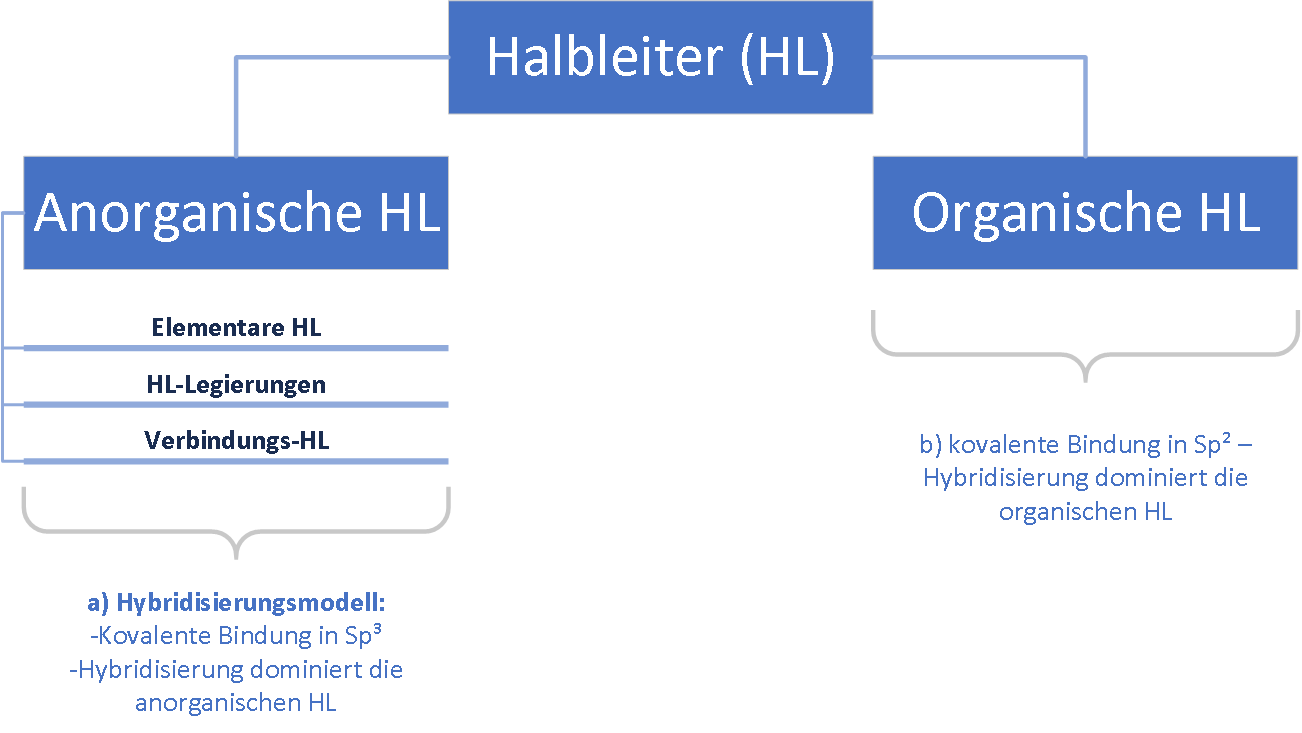
\includegraphics[width=0.9\textwidth]{Halbleiterklassen.png}
		    \caption{Halbleiterklassen}
		    \label{fig:halbleiterklassen}
      \end{figure}
		  \begin{definition}
		    Halbeiter: Ein Material, das grundsätzlich leitfähig ist und dessen Verhalten bei Erhitzung metallischer und beim absoluten Nullpunkt isolierend wird.
		  \end{definition}
		  
		  \subsubsection{Bindungen - Elektronenpaarbindung} \label{sss:elpaar}
		  Beim Nullpunkt sind alle Bindungen fest. Bei Erhitzung muss um das die Bindung zu lösen dem Elektron so viel Energie zugefügt werden, dass es aus der Bindung herraus "geschossen" wird.
		  \begin{figure}[H] 
		    \centering
		    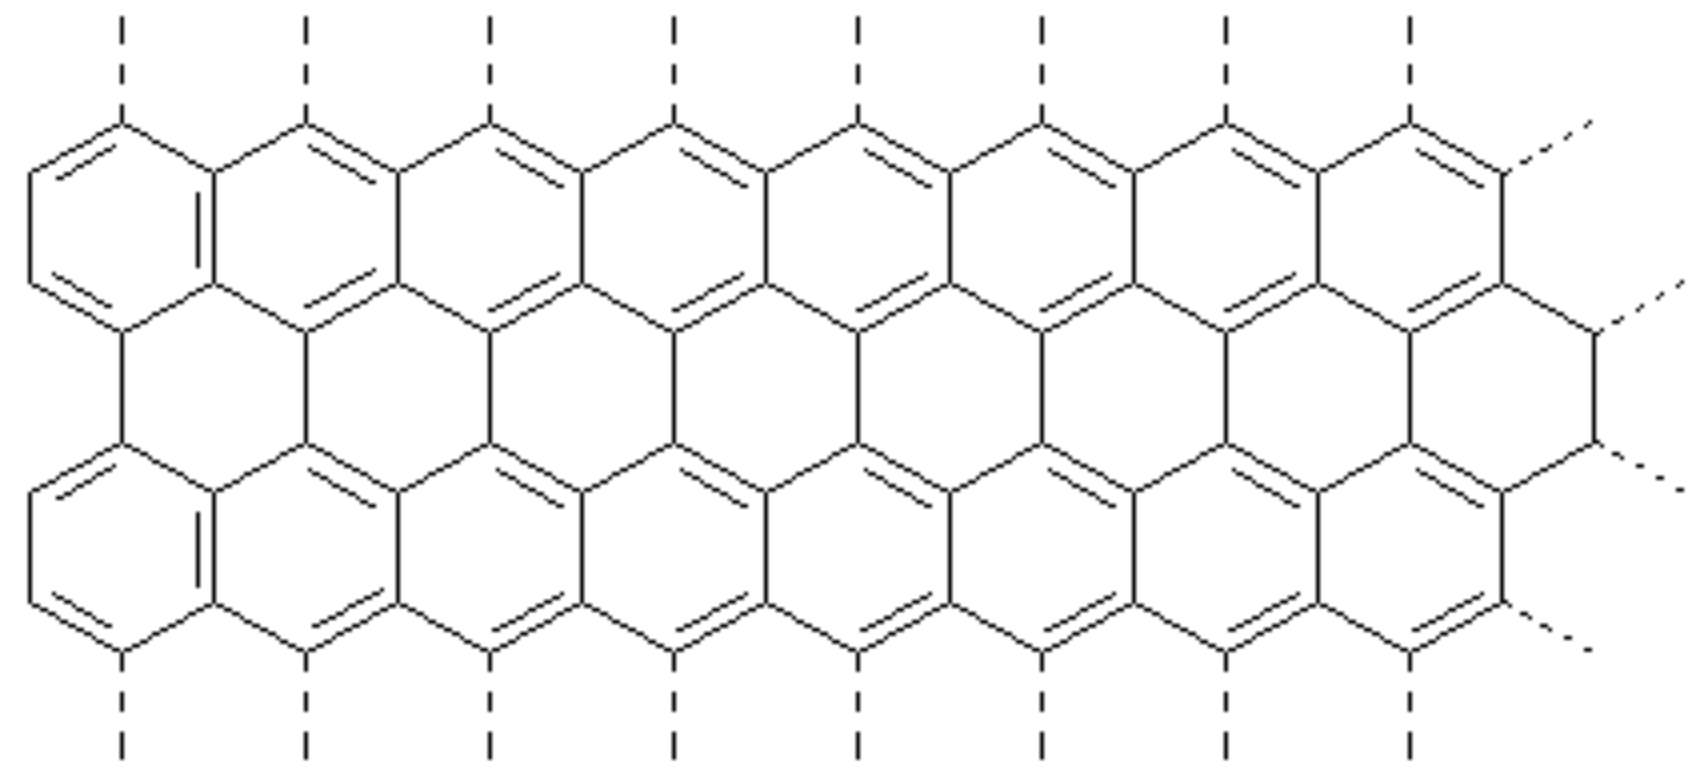
\includegraphics[width=0.7\textwidth]{graphen.png}
		    \caption{Wabenstruktur} \cite{waben}
		    \label{fig:wabenstruktur}
      \end{figure}
\newpage
\section{17. April 2018: Vorlesung 2}
		\begin{bem}
		  Zu \eqref{sss:elpaar}: Elektronenpaarbindungen entsprechen Doppelbindungen.
		\end{bem}
		$\;$\newline
		Üblich ist $Sp^3$ Hybridisierung, Kohlenstoff kann aber auch $Sp^2$ Hybride bilden.
		
		\subsection{Silizium: Das Material der modernen Mikroelektronik}
		\subsubsection{Transistortypen}
		\begin{definition}
		  BJT: \ul{B}ipolar \ul{J}unction \ul{T}ransistor bzw. Bipolartransistor\newline
		  CMOS: \ul{C}omplementary \ul{M}etal \ul{O}xide \ul{S}emicoductor
		\end{definition}
		\begin{bem}
		  Transistortypen: NPN bzw. komplementär dazu PNP.
		\end{bem}
		\begin{definition}
		  Transistor: \ul{Trans}fer Resis\ul{tor}
		\end{definition}
		\begin{definition}
		  Complementary: Innen Elektronen, aussen Löcher. Kleiner Elektronenstrom an der Basis um großen Strom anzutreiben. 
		\end{definition}
		
		\subsubsection{Weltmarkt}
		\begin{itemize}
		  \item 95\% Si-basiert, davon knapp 90\% CMOS
		  \item 90\% aller hergestellten Bauelemente sind Transistoren
		  \item Von 10\€ wird 1\€ weltweitl mit Halbleitern verdient
		  \item Nach Sauerstoff ist Silizium das zweithäufigste Element (Sand = Siliziumdioxid, im Allgemeinen wird Quarzsand aus dem Bergbau verwendet, siehe Mikro 1)
		  \item 1kg Si < 10\€ im Vergleich zu 4000\€ - 5000\€ um 500gr Arsen zu gewinnen
		  \item Bei einer Umstellung auf GaAs könnte man ca. 10 Tage die Fertigung aufrecht erhalten, danach wären alle Rohstoffe verbraucht
		  \item FET Technologie funktioniert mit Germanium nicht, nur mit Silizium
		\end{itemize}
		
		\subsubsection{Fünf Gründe für die Dominanz von Silizium}
		\begin{itemize}
		  \item[1) ] Si ist ein Elementarhalbleiter
		  \begin{itemize}
		    \item Substrat entspricht Wafermaterial
		    \item Leichte Substratherstellung
		  \end{itemize}
		  \item[2) ] Man findet Si praktisch "wie Sand am Meer" (wenn auch nicht ganz da hauptsächlich Quarzsand verwendet wird)
		  \begin{itemize}
		    \item $\rightarrow$ Kostengünstig, "unbegrenzt" verfügbar
		    \item Bipolar: Löcherstrom und Elektronenstrom
		    \item Atome pro $cm^{-3}$: $10^{23}$
		    \item Dotieren nicht unterhalb der intrinsischen Grenze $\sim 10^{10}$ (gilt nur bei RTP)
		  \end{itemize}
		  \item[3) ] Si lässt sich in einem sehr weiten Bereich von $10^{15} - 10^{20} \frac{1}{cm^3}$ dotieren
		  \item[4) ] Si ist ungiftig
		  \item[5) ] Si bildet mit SiO2 einen elektrisch perfekten Isolator $\Rightarrow$ MOSFET-Technologie möglich
		  \item[6) ] Schutz der Investition
		  \begin{itemize}
		    \item Moderne Halbleiter-Fabrik kostet ungefähjr 3 Milliarden\€
		    \item Betrieb ca. 2 Millionen \€
		  \end{itemize}
		\end{itemize}
		
		\subsection{Some facts}
		\begin{itemize}
		  \item Der erste Transistor wurde 1938 von Robert Wichard Pohl und Rudolf Hilsch der erste Transistor aus Kalium-Bromid hergestellt. Das Material war aber eher ungeeignet, da es wasserlöslich ist.
		  \item Der BP (Bipolar) Transistor ist sehr viel schneller als der MOSFET, daher in vor allem in der HF (Hochfrequenz) Technik häufig genutzt
		  \item MOSFETs können als normally on/off umgesetzt werden. Am gebräuchlichsten ist normally off
		\end{itemize}
		\newpage
	
	\section{24. April 2018: Vorlesung 3}
	  \begin{itemize}
	    \item[1) ] Natürliche Zahlen $\N = \lbrace 1,2,3,...,\infty \rbrace$\newline
	      Natürliche Zahlen sind natürlich da sie einfach 'da' sind. Alle anderen Zahlenmengen sind aus den natürlichen Zahlen heraus gebaute Konstrukte.
	    \item[2) ] Verknüpfungen werden definiert (allgemein $*$)
	    \begin{itemize}
	      \item Additiv
	      \item Multiplikativ
	    \end{itemize}
	    \begin{align*}
	      a * b \rightarrow c 
	    \end{align*}
	      Bei der Verknüpfung darf die Menge nicht verlassen werden (Abgeschlossenheit), d.h. $a,b \in \N \Rightarrow c \in \N$. \newline
	      Addition und Multiplikation sind in $\N$ abgeschlossen, Division und Subtraktion allerdings nicht. Zur Erweiterung der Menge müssen das neutrale Element und das inverse Element definiert werden (siehe HM1).
	      \begin{itemize}
	        \item Neutrale Elemente $\qquad$
	        \begin{tabular}{l | r}
	          Erweiterung von $\N$ zu $\Z$ & Erweiterung von $\N$ zu $\Q$\\
	          $a - a =: 0$                 & $a \cdot a^{-1} = e$ \\
	          $a + 0 = 0 + a = a $         & $e \cdot a = a \cdot e = a$ 
	        \end{tabular}
	      \end{itemize}
	    \item[3) ] Begriffe: Gruppe, Ringe, Körper
		    \begin{itemize}
		      \item Die einfachste algebraische Struktur ist die Gruppe. Dann kommt der Ring und danach der Körper.
		      \item Gruppe: Vereinigung einer Zahlenmenge und einer Verknüpfung
		      \item Abelsche Gruppe: Ist eine Gruppe weiterhin kommutativ ist sie abelsch
		      \item Ring: Vereinigung aus einer Zahlenmenge und zwei Verknüpfungen (additiv und multiplikativ); Wortherkunft: Verbund von Elementen die untereinander unterschiedlich sind aber eine Aufgabe erfüllen(z.B. Verbrecherring)
		      \item Körper: Alle Eigenschaften von Ringen und zusätzlich Distributivität.
		    \end{itemize}
	    \item[4) ] $\Q \rightarrow \R$: Cauchy-Folge (erzeugt Relle Zahlen, konvergiert gegen jede denkbare irrationale Zahl)
	    \item[5) ] Komplexe Zahlen
			    \begin{align*}
			      \sqrt{b} &= ?  \text{ für } b < 0\\ 
			      a:\; a * a &= b\\
			      \sqrt{-1} &=: i \text{ bzw. in der Elektrotechnik oftmals } j \\
			      \Rightarrow \C: \Z &= a+ib \qquad a,b \in \R\\
			      Re\lbrace Z \rbrace &= a \qquad Im\lbrace Z \rbrace = b
			    \end{align*}
			    $\Rightarrow$ Vorteil: Real- und Imaginärteil immer getrennt
	    \item[6) ] Gibt es n-dimensionale Zahlen?
	      \begin{align*}
	        y = a + ib + kc,\qquad \sqrt{i} = \sqrt{k} = -1, \qquad a,b,c \in \R
	      \end{align*}
	      Fügt man noch einen weiteren Term an erhält man die Quaternionen mit denen gerechnet werden kann.
	    \item[7) ] Abbildungen:
	    \begin{align*}
	      \lbrace M \rbrace f: M \rightarrow N \lbrace N \rbrace 
	    \end{align*}
	  \end{itemize}
	  \begin{definition}
	    Algebra: Aus dem arabischen von \textit{al-\u{g}abr} abgeleitet. Es bedeutet im übertragenen Sinne 'das Zusammenfügen gebrochener Teile', kann aber auch einfach als 'Rechnen' interpretiert werden.
	  \end{definition}
	  \subsection{Die Arbeitsweise des Computers}
	  Notwendig für ein Computer auf Basis von Binärzahlen:
	  \begin{align*}
	    \R \overset{f}{\rightarrow} B,\qquad \text{ mit } B \text{ als Menge der Binärzahlen}
	  \end{align*}
	  Notwendige Bedingung damit die Abbildung geeignet ist: $f$ muss ein \textit{bijektiver Homomorphismus} sein, was nichts anderes als ein \textit{Isomorphismus}.
	  \begin{definition}$\;$\newline
	    Morphologie: Struktur (Form)\newline
	    Homo: Gleich im Sinne von ähnlich \newline
	    Iso: Gleich im Sinne von identisch\newline
	    Homomorphismus: Ähnlich in der Struktur \newline
	    Isomorphismus: Identisch in der Struktur \newline
	  \end{definition}
	  D.h. es muss bewiesen werden, dass die Menge der binären Zahlen die gleiche algebraische Struktur aufweisen, wie die Menge der reellen Zahlen aus der sie konstruiert wurde (also ein Zahlenkörper).
	  Dazu:
	  \begin{align*}
	    a,b \in \R&\qquad a * b = c\\
	    f(a) = b_a \qquad f(b) &= b_b \qquad b_a * b_b = \tilde{x} \\
	    \Rightarrow c &= f^{-1}(\tilde{x})
	  \end{align*}
	  Beispiel:
	  \begin{align*}
	    a &= 13, \quad a\in \R \\
	    B: b_a &= \sum\limits_{i = -n}^{+m} \alpha_i 2^i  \qquad \alpha_i \in \lbrace 0,1 \rbrace 
	  \end{align*}
	  Darstellung:
	  \begin{align*}
	    &Z_m Z_{m-1} ... Z_0, Z_{-1} ... Z_{-n} \\
	    &\Rightarrow 13 \rightarrow 
	    \begin{array}{c c c c}
	      2^3 & 2^2 & 2^1  & 2^0 \\
	      8   & 4   & 2    & 1   \\ \hline
	      1   & 1   & 0    & 1
	    \end{array}
	    \Rightarrow 13  \rightarrow 1101
	  \end{align*}
	  Die Algebra auf der Menge der Binärzahlen wird \textit{boolesche Algebra} genannt (Logik).
	  \subsection{Standard Gatter}
	  Das AND-Gatter:
	  \begin{figure}[H] 
		\centering
		\begin{minipage}{.5\textwidth}
		  \centering
		  \captionsetup{justification=centering}
		  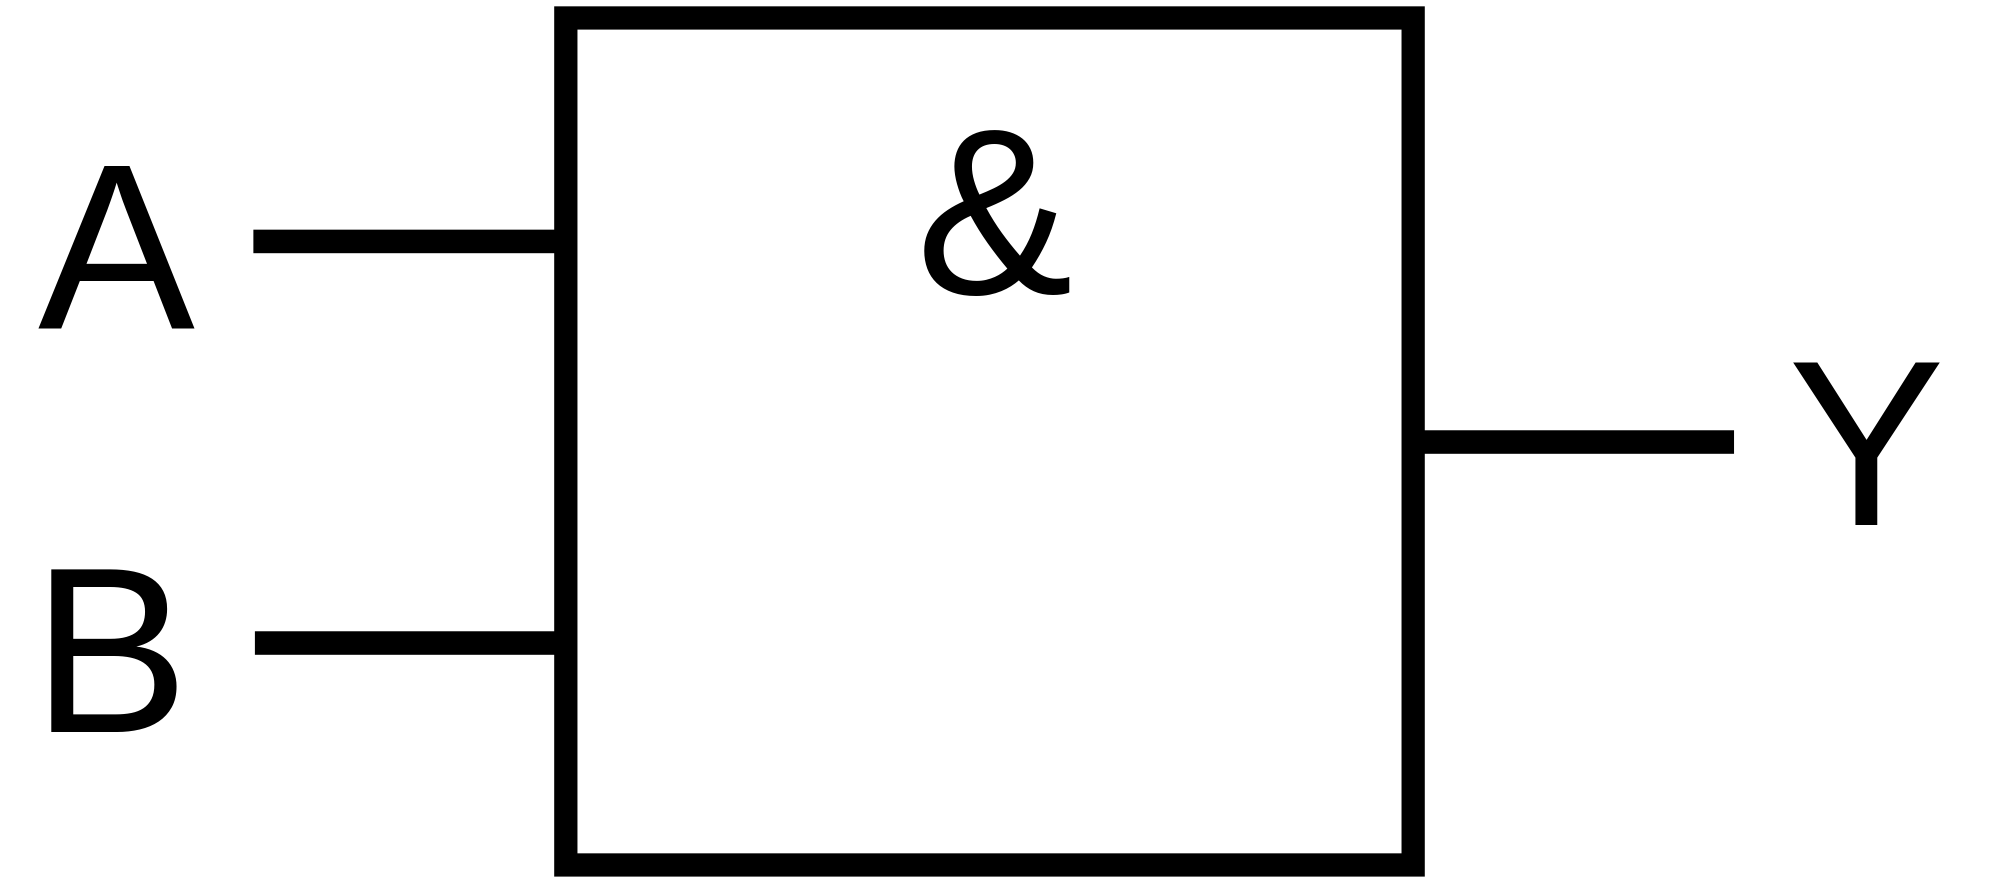
\includegraphics[width=0.6\linewidth]{AND.png}
		  \caption{AND-Gatter (deutsche Darstellung)}
		  \label{fig:and_de}
		\end{minipage}%
		\begin{minipage}{.5\textwidth}
		  \centering
		  \captionsetup{justification=centering}
		  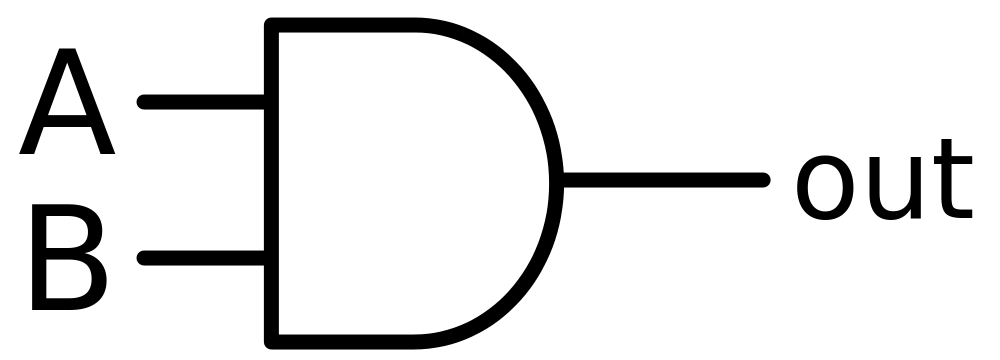
\includegraphics[width=0.6\linewidth]{AND_int.png}
		  \caption{AND-Gatter (international)}
		  \label{fig:and_int}
		\end{minipage}
  \end{figure}
  \begin{table}[H]
	  \centering
	  \begin{tabular}{c | c c c} 
	    AND & A(In 1) & B(In 2) & Y(Out) \\ \hline
	    $\;$& 0       & 0       & 0 \\   
	    $\;$& 0       & 1       & 0 \\   
	    $\;$& 1       & 0       & 0 \\   
	    $\;$& 1       & 1       & 1 \\   \hline
	  \end{tabular}
  \end{table}
  Verknüpft man ein AND-Gatter mit einer Negation erhält man das NAND-Gatter (über das sämtliche logische Verknüpfungen realisiert werden können):
  \begin{figure}[H] 
		\centering
		\begin{minipage}{.5\textwidth}
		  \centering
		  \captionsetup{justification=centering}
		  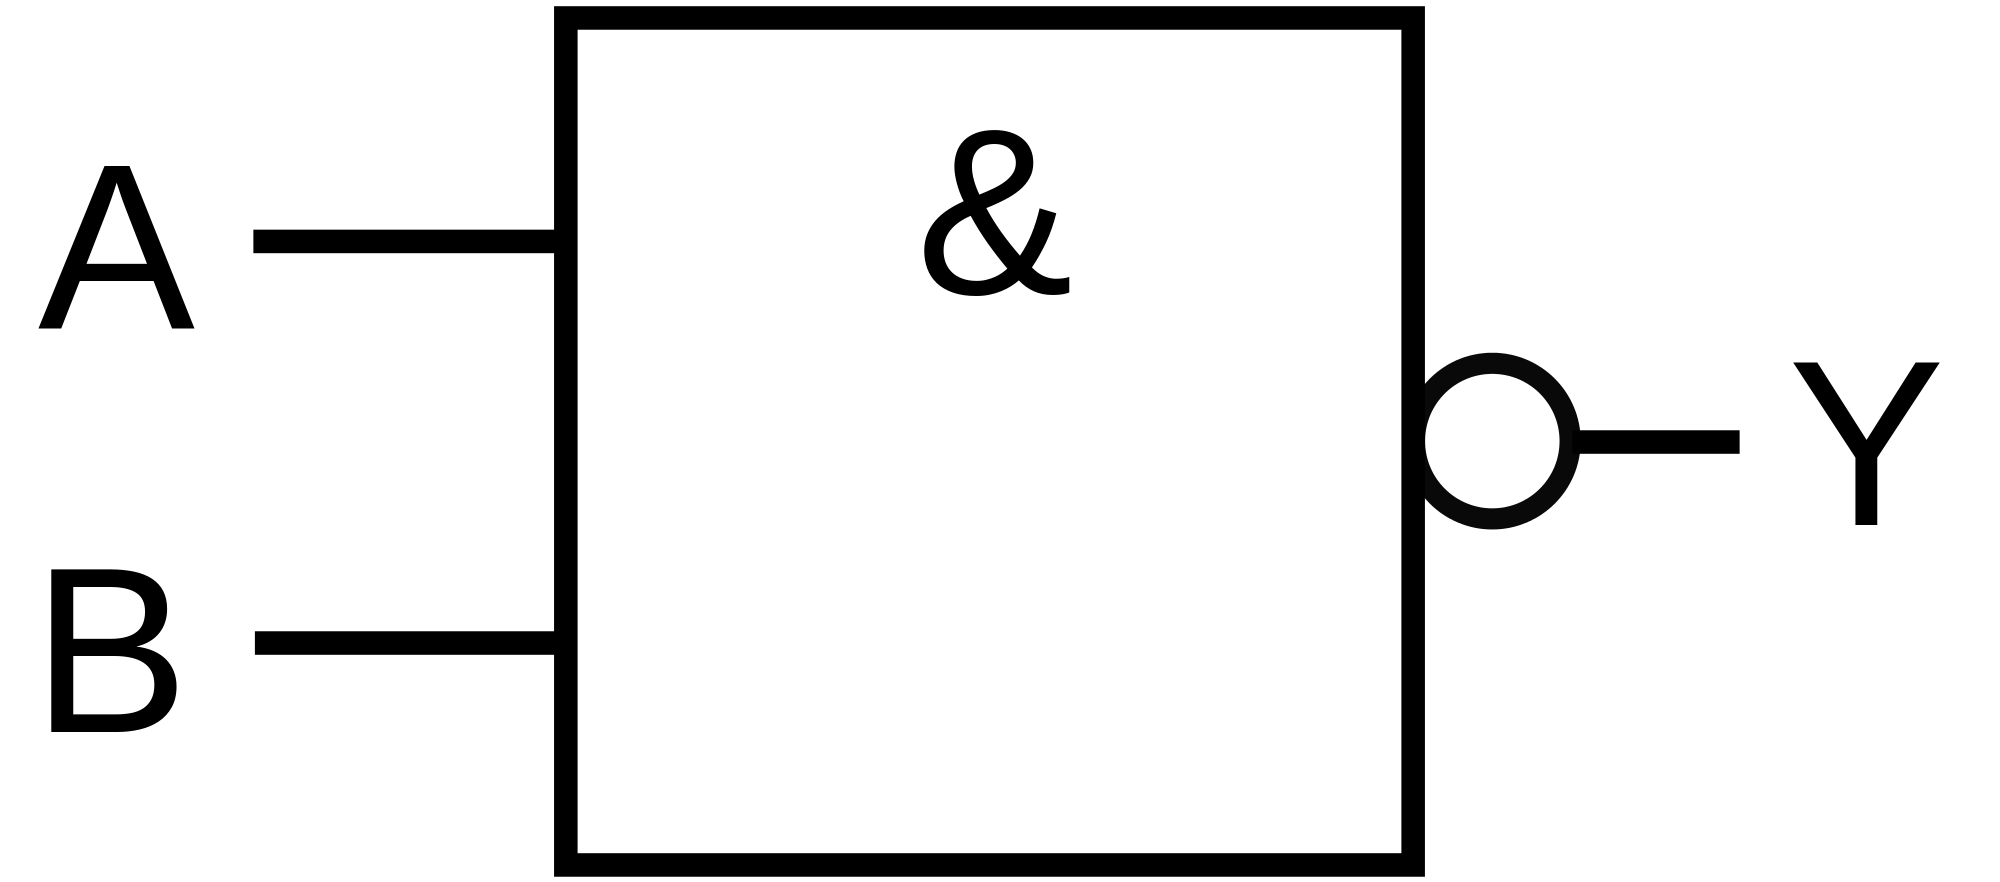
\includegraphics[width=0.6\linewidth]{NAND.png}
		  \caption{NAND-Gatter (deutsche Darstellung)}
		  \label{fig:nand_de}
		\end{minipage}%
		\begin{minipage}{.5\textwidth}
		  \centering
		  \captionsetup{justification=centering}
		  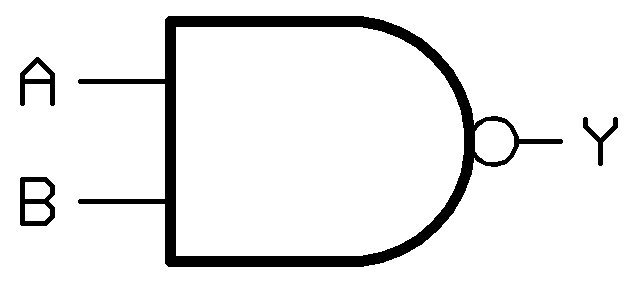
\includegraphics[width=0.6\linewidth]{NAND_int.png}
		  \caption{NAND-Gatter (international)}
		  \label{fig:nand_int}
		\end{minipage}
  \end{figure}
  \begin{table}[H]
	  \centering
	  \begin{tabular}{c | c c c} 
	    NAND & A(In 1) & B(In 2) & Y(Out) \\ \hline
	    $\;$& 0       & 0       & 1 \\   
	    $\;$& 0       & 1       & 1 \\   
	    $\;$& 1       & 0       & 1 \\   
	    $\;$& 1       & 1       & 0 \\   \hline
	  \end{tabular}
  \end{table}
\newpage

	\section{08. Mai 2018: Vorlesung 4}
	\subsection{Areniusplot}
	\begin{figure}[H] 
	  \centering
	  \captionsetup{justification=centering}
	  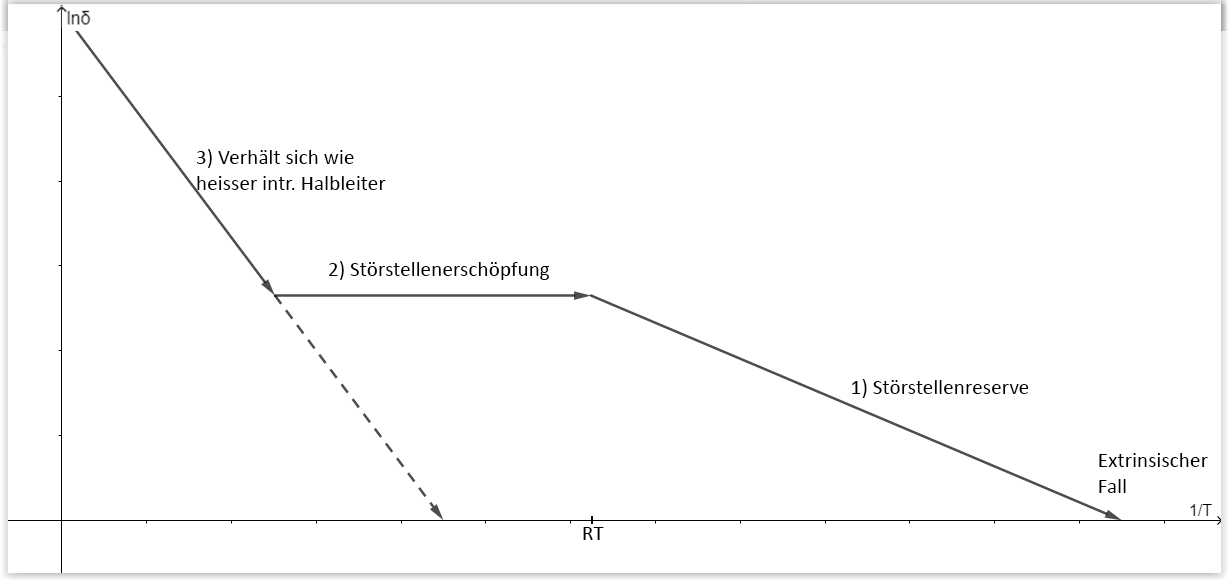
\includegraphics[width=0.9\linewidth]{Areniusplot.png}
	  \caption{Areniusplot}
	  \label{fig:areniusplot}
  \end{figure}
  Der Areniusplot (hier dotiert) stellt die Temperatur und die Leitfähigkeit ins Verhältnis (Achtung, $\ln \sigma$ und $\frac{1}{T}$). Es gilt:
  \begin{align*}
    n(t) \sim \displaystyle e^{-\displaystyle\frac{E}{K_B T}}
  \end{align*}
  Die gestrichelte Linie stellt das Verhalten dar, das ein intrinsischer Halbleiter hätte.
  \begin{itemize}
    \item[1) ] Störstellenreserve: Die Dotieratome (z.B. Phosphor) geben ihre zusätzliches Elektron ab. Das läuft solange ab bis alle Dotieratome ihr Elektron abgegeben haben.
    \item[2) ] Störstellenerschöpfung: Dotieratome haben alle ihr zusätzliches Elektron abgegeben, Energie ist aber noch zu niedrig um weitere Bindungen aufzubrechen.
    \item[3) ] Energie ist hoch genug, dass Bindungen zwischen Silizium und Phosphor aufbrechen, Halbleiter wird mit Elektronen so stark überschwemmt dass die Dotierung keine Rolle mehr spielt (daher Verhalten wie im intrinsischen Fall) und es gilt $n\sim p$.
  \end{itemize}
  Im Bereich 1) arbeitet der Chip nicht mehr zuverlässig. Gewünscht ist der Bereicht um RT (Raumtemperatur). 
  \subsection{Verlustleistung}
  Durch permanente Miniaturisierung wurde die Leistung der Chips höher, dabei wird aber auch mehr Abwärme durch Verlustleistung produziert.
  Abschätzung der Verlustleistung in einem N(P)Mos-Inverter. Folgende Annahmen sind zu treffen:
  \begin{itemize}
    \item[1) ] N-Inverter miteinander verschaltet
    \item[2) ] Pro Takt sind $\frac{N}{2}$ der FETs im Off- bzw. On-Zustand
    \item[3) ] $I_{stat} = I$
  \end{itemize}
  \begin{equation}
    \Rightarrow P_{total} \cong \frac{N}{2} I \cdot V_{cc} + N \cdot I_{dyn} V_{cc} \label{eq:p_tot_N}
  \end{equation}
  Hier ist die Verlustleistung als Funktion der Anzahl der Inverterstufen gegeben.
  
  \subsection{Moores Law}
  \begin{itemize}
    \item Formuliert durch Gordon E. Moore in 1965
    \item Beobachtung: Vervierfachung der Anzahl der Transistoren auf einem Chip alle drei Jahre
  \end{itemize}
  
  \subsection{Some facts}
  \begin{itemize}
    \item Erstes kommerzielles transistorbasiertes Produkt: Texas Instruments Taschenrechner
    \item Schmelztemperatur Si: $1400^{\circ}$
    \item 1 Angström entspricht $1 \cdot 10^{-10}m$
    \item Bei Transistorgrößen < 5nm überwiegen quantenmechanische Eigenschaften $\Rightarrow$ undeterministisches Verhalten
  \end{itemize}
\newpage

	\section{15. Mai 2018: Vorlesung 5}
  \begin{align}
    \text{\eqref{eq:p_tot_N} } &= \frac{N}{2}I \cdot V_{cc} + N \cdot C_L  \cdot f \cdot V_{cc}^2 \nonumber \\
    \overset{\text{Umbau von MOS in CMOS}}{\rightarrow} \nonumber \\ 
    P_{total} &\cong N C_L f V_{cc}^2 \label{eq:p_tot_cmos}
  \end{align}
  Wachstum von $N$ und $F$ ist exponentiell, daher werden die Chips immer heißer, was immer effizienteres Kühlen erforderlich macht. Die Lösung ist der CMOS, da hier der statische Verluststrom weg fällt (da der CMOS im ausgeschalteten Zustand so gut sperrt, dass praktisch kein Strom fließt). Somit wird auch die Temperatur in der der HL in den intrinsischen Modus verfällt später erreicht.
  
  \subsection{Komplementär}
  \begin{definition}
    Zwei elektronische Bauelemente heißen komplementär zueinander, wenn der Verlauf der Kennlinie erhalten bleibt, sich jedoch das Vorzeichen invertiert. 
  \end{definition}
  \begin{figure}[H] 
	  \centering
	  \captionsetup{justification=centering}
	  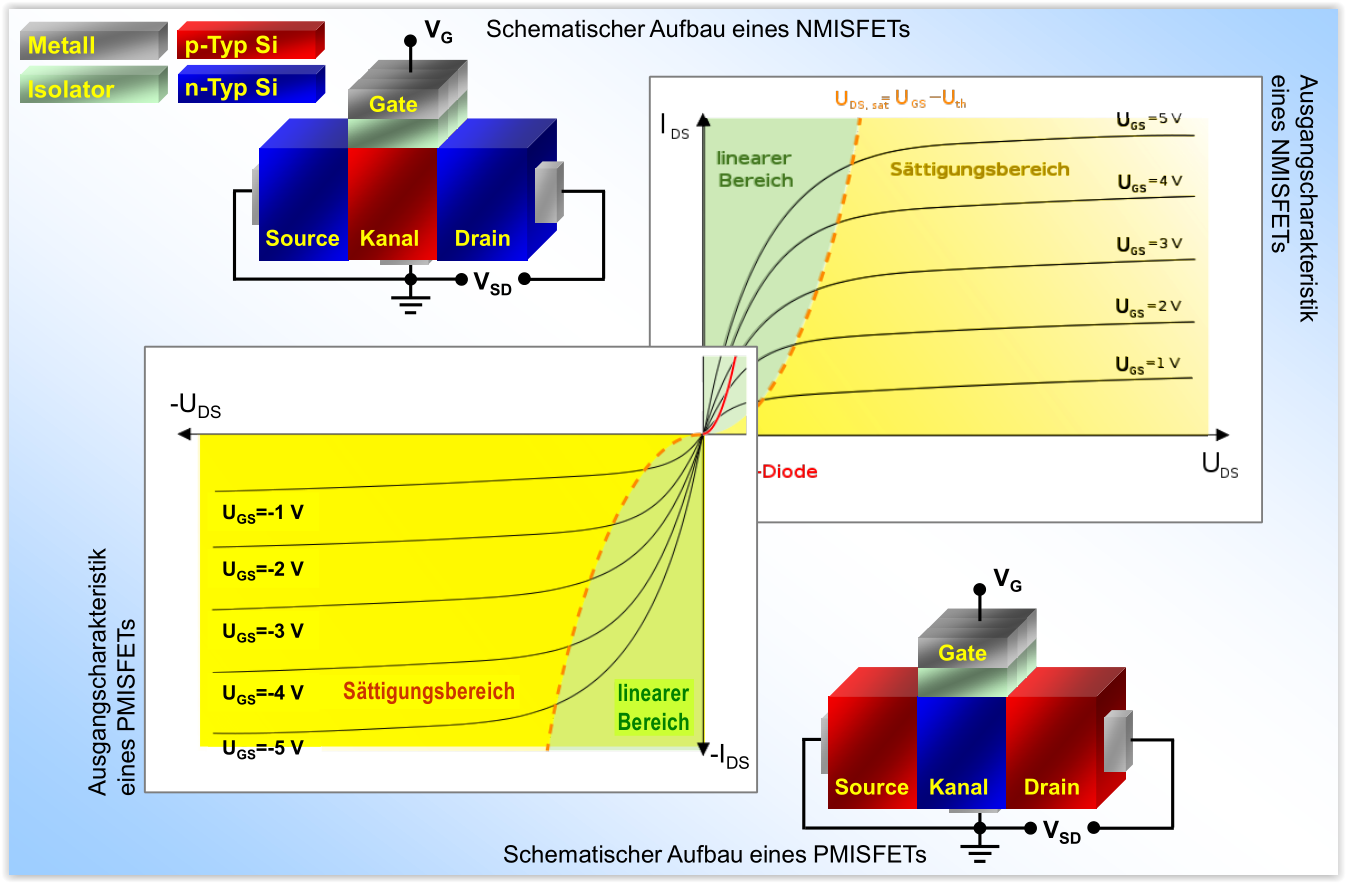
\includegraphics[width=0.9\linewidth]{pnp_npn_kennlinie.png}
	  \caption{Kennlinie komplementär \protect\cite{MIKRO2}}
	  \label{fig:komplementaer}
  \end{figure}
  
  Aus \eqref{eq:p_tot_cmos} folgt wiederrum 
  \begin{equation}
    \rightarrow \frac{P_{total}}{C_L V_{cc}^2} = N \cdot f = konstant
  \end{equation}
  Hierbei spricht man vom "Power Delay Produkt". Zwischen $N$ und $f$ findet ein "Tradeoff" statt. Da das Produkt konstant ist, kann keiner der beiden Faktoren beliebig erhöht werden. Wird $N$ erhöht so muss $f$ gesenkt werden und umgekehrt. Das "Power Delay Produkt" kann weiterhin wie folgt beschrieben werden:
  \begin{equation}
    \text{Power Delay Produkt: } \ln (Nf) = \ln (N) + \ln (f) = \ln (konst) = konst
  \end{equation}
  
  \subsection{Speichertypen}
  Die meistgenutzten Speichertypen sind:
  \begin{table}[H]
    \centering
    \begin{tabular}{c | c}
    SRAM & DRAM \\ \hline
    \ul{S}tatic \ul{R}andom \ul{A}ccess \ul{M}emory & \ul{D}ynamic \ul{R}andom \ul{A}ccess \ul{M}emory \\
    Schneller aber teurer & Langsamer aber günstiger \\
    Flip Flop basiert & Kondensatorbasiert
    \end{tabular}
  \end{table}
  
  \subsection{Thyristoren}
  \begin{itemize}
    \item Verschachtelung von PNP und NPN Bipolartransistoren
    \item Drei PN Übergänge und damit drei Schottky Kontakte
    \item Einmal angeschaltet geht der Thyristor erst bei $0V$ wieder aus
    \item Awendungsgebiet: Hochspannung $\sim 800kV$
  \end{itemize}

  \subsection{Bindung und Strukturen}
  Die Elemente Kohlenstoff, Silizium, Germanium und weitere haben die gleiche Kristallstruktur, verhalten sich aber unterschiedlich. Graphit lässt sich selbst in unterschiedliche Strukturen bringen die alle ein anderes Leitverhalten vorweisen. Polykristallin ist Graphit leitend, monokristallin lässt sich das Verhalten nur noch durch einen Tensor beschreiben. 
   \begin{figure}[H] 
	  \centering
	  \captionsetup{justification=centering}
	  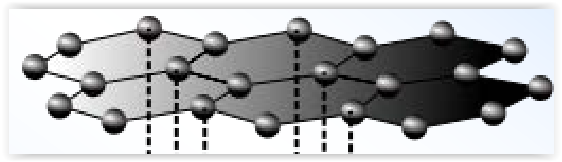
\includegraphics[width=0.6\linewidth]{graphen_b.png}
	  \caption{Monokristalline Graphitlage \protect\cite{MIKRO2}}
	  \label{fig:graphen_a}
  \end{figure}
  Legt man ein elektriches Feld horizontal an weißt das Material eine extrem gute Leitfähigkeit auf. Legt man das Feld vertikel an so wirkt das Material wie ein Isolator.
  Man Spricht hier von einem anisotropen Leitverhalten.
  \begin{definition}$\;$ \newline
    Iso: gleich \newline
    Trop: Raum \newline
    Isotrop leitend: Im Raum in allen Richtungen gleich leitend\newline
    Anisotrop leitend: Im Raum in unterschiedlichen Richtungen unterschiedlich gut leitend $\rightarrow$ Leitfähigkeitstensor
  \end{definition}
  
  \subsection{Some facts}
  \begin{itemize}
    \item PNP üblicherweise breiter als NPN da die Beweglichkeit von Löchern kleiner als die von Elektronen ist\newline
    $\rightarrow$ bei gleicher Baugröße treibt ein PNP Transistor weniger Strom als ein NPN Transistor
    \item Eine Elektronenpaarbindung ist eine kovalente Bindung
    \item Zinn ist ein sogenanter Zero-Bandgap Halbleiter, also ein Halbleiter bei dem die Bandlücke $0eV$ beträgt. Er verhält sich somit metallisch und wird auch als Halbmetall bezeichnet.
  \end{itemize}
\newpage

	\section{Einschub Graphen/Kohlenstoffnanoröhrchen}
	\subsection{Kristallstrukturen und Eigenschaften von Graphit}
    Graphit lässt sich in unterschiedlichen Strukturen vorfinden, die allesamt unterschiedliche Eigenschaften, insbesondere mit Bezug auf das Verhalten als Leiter, Halbleiter oder nichtleiter, haben. 
    %\subsubsection{Amorphe Struktur}
    Von amorphem Kohlenstoff spricht man, wenn die Atome ohne eine langreichweitige Ordnung vernetzt sind. Weder aus der Ferne, noch aus der Nähe erkennt man eine Struktur im Material. \newline
    %\subsubsection{Polykristalline Struktur}
    
    Um einen polykristallinen Graphitblock herzustellen, komprimiert man mehrere Bruchstücke eines Graphitkristalls zu einer festen Struktur. Bei der Betrachtung in der Nähe erkennt man so eine perfekte Kristallstruktur, bei der Betrachtung aus der Ferne jedoch sieht man allerdings die abrupten Übergänge der einzelenn Bruchstücke. Dadurch ist polykristalliner Graphit schlechter leitfähig als in monokristalliner Form.\newline
    %\subsubsection{Monokristalline Struktur}
    
    Ein monokristalliner Graphitblock ist ein gewachsener Graphitkristall, der sowohl in  der Nähe als auch in der Ferne eine perfekte Kristallstruktur aufweißt. Die Leitfähigkeit eines solchen monokristallinen Graphitblocks ist abhängig von der Lage des elektrischen Felds bezüglich zu den einzelnen Kristallschichten. Zur korrekten Beschreibung ist ein Tensor zweiter Ordnung nötig. Parallel zu den Schichten weißt ein monokristalliner Graphitblock eine sehr gute, beinahe metallische Leitfähigkeit von $0,03\cdot 10^6 \frac{S}{cm}$ auf \citevgl{Weinschenk1898Graphitseine}.Vertikal zu den Schichten verhält er sich nahezu wie ein Isolator.
    
  \subsection{Graphen}
  Mit Graphen bezeichnet man ein 1 Atom dickes, hexagonales Kohlenstoffgitter. Sogesehen ist Graphen eine Kristallschicht eines monokristallinen Kohlenstoffblocks. Dabei zeigt Graphen Eigenschaften, die es für eine mechanische und elektrotechnische Nutzung interessant machen. Es ist einerseits mit $\SI{3,35}{\angstrom}$ und einer Dichte von $0,77 \frac{mg}{m^2}$ ultimativ dünn, weist aber andererseits eine mit $42 \frac{N}{m}$ im Vergleich zu Stahl ($0,4 \frac{N}{m}$) sehr hohe Bruchstärke auf \citevgl{Chandrasekhar2018ConductingPolymers}. Weiterhin zeichnet sich das Material durch eine elektrische Leitfähigkeit von $0,96\cdot10^6 \frac{S}{cm}$ aus und übertrifft damit die Leitfähigkeit von Kupfer mit $0,60\cdot 10^6 \frac{S}{cm}$ deutlich\citevgl{Chandrasekhar2018ConductingPolymers}. Ähnlich verhält es sich bei der thermischen Leitfähigkeit, bei der Graphen mit $ \approx 5000WK^{-1}m^{-1}$ ebenfalls deutlich leitender als Kupfer mit $\approx 400WK^{-1}m^{-1}$ ist\citevgl{Chandrasekhar2018ConductingPolymers}.
  \newpage
  \subsection{Kohlenstoffnanoröhren}
  Die Wände einer Kohlenstoffnanoröhre bestehen wie Graphen aus einer 1 Atom dicken Kohlenstofflage. Somit kann man sich Kohlenstoffnanoröhren wie ein kleines Stück Graphen, dass zu einer Röhre aufgerollt wurde, vorstellen. Üblicherweise liegen die Durchmesser der Röhren in einem Bereich von $1-50nm$, die kleinsten bisher hergestellten Röhren haben einen Durchmesser von $0,4nm$\citevgl{Fujita2013Electricalconduction}. Dabei sind in der Herstellung Längen von bis zu einem halben Meter realisierbar \citevgl{Fujita2013Electricalconduction}.\newline
  
  Es sind zwei Unterarten von Kohlenstoffnanoröhrchen (CNT = carbon nanotubes) zu unterscheiden, mit denen ein hoher Grad an struktureller Perfektion erreicht werden kann. Sogenannte single-walled nanotubes (SWNTs) bestehen aus einer einzelnen Kristalllage, die zu einem Zylinder aufgerollt ist. Multi-walled nanotubes (MWNTs) bestehen dagegen aus einer konzentrischen Anordnung mehrerer SWNTs. Aufgrund dieser Anordnung können unterschiedliche Leitertypen erzeugt werden und somit das grundsätzliche Verhalten der CNTs angepasst werden.\citeVgl{Baughman787}
    \subsubsection{Strukturen}
      Je nach Verscherung bzw. Atomanordnung der Kristalllage der Röhrchen ist es möglich die Leitfähigkeit stark zu beeinflussen. Man spricht hier hauptsächlich von drei Typen. Armchair CNTs weisen ein metallisches Verhalten auf, Zigzag CNTs dagegen halbleitende Eingeschaften \citevgl{Chandrasekhar2018ConductingPolymers}. Die folgende Graphik zeigt die unterschiedlichen Strukturen der Wabenanordnung, die auch namensgebend für die jeweiligen Typen ist.
		\begin{figure}[H] 
		  \centering
		  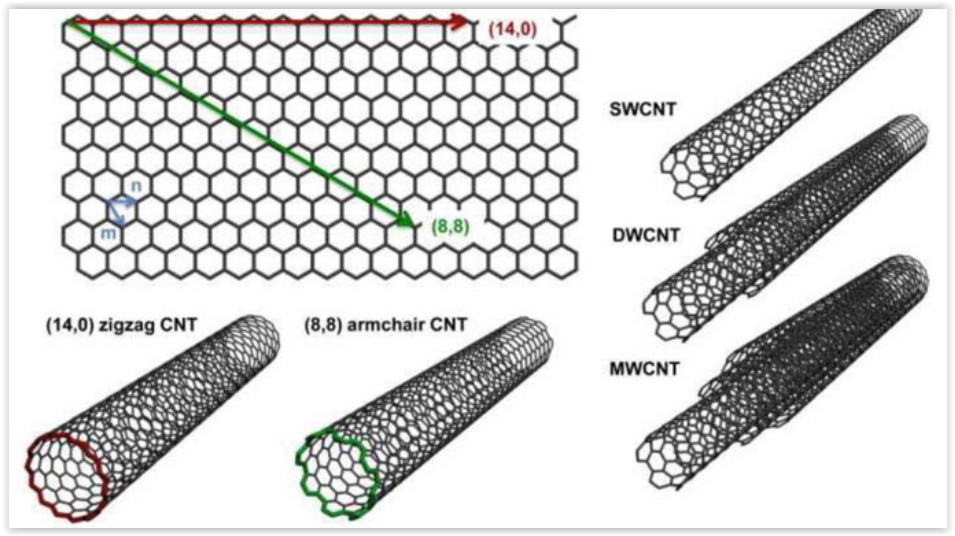
\includegraphics[width=0.7\textwidth]{structures.png}
		  \caption{Strukturen von Kohlenstoffnanoröhrchen\protect\cite{Chandrasekhar2018ConductingPolymers}}
		  \label{fig:cnt_structures}
		\end{figure}
		%\newline
		Eine weitere gängige Form Chiral CNTs. Dabei handelt es sich um Armchair CNTs, die verschert aufgerollt wurden. Chiral CNTs weisen wie Zigzag CNTs halbleitende Eigenschaften auf.
\newpage

	\section{29. Mai 2018: Vorlesung 6}
	\begin{definition}
	  Morph: Form\newline
	  a: ohne\newline
	  Amorph: Ohne Form
	\end{definition}
	\begin{table}[H]
	  \centering
	  \begin{tabular}{c | c}
	    Polykristallin & Monokristallin \\ \hline
	    Nur in Nahordnung wie ein gewachsener Kristall & Einzelner komplett gewachsener Kristall \\
	    In Fernordnung unregelmäßig & Nah- und Fernordnung absolut regelmäßig
	  \end{tabular}
	\end{table}
	
	  \subsection{Monokristallines Si}
	  \setlength{\jot}{-10pt}
	  \begin{align}
	    &\; \qquad \qquad \vv{j} = \underbrace{\vv{\sigma}}_{\;}\vv{\varepsilon} \\ 
	    &\text{Bei monokristallinem Si Tensor 2. Ordnung} \nonumber
	  \end{align}
	  \setlength{\jot}{3pt}
	  Trägheitstensor für monokristallines Si:
	  \begin{equation}
	    \vv{\sigma} = \left(
	    \begin{array}{c c c}
	      \vv{\sigma} & 0 & 0 \\
	      0 & \vv{\sigma} & 0 \\
	      0 & 0 & 0
	    \end{array}
	    \right)
	  \end{equation}
	  
	  \subsection{Atomaufbau}
	  Vergleich zur Mechanik und Elektrodynamik:
	  \begin{align}
	    \text{Gravitation: } \vv{F_G} &= -\gamma \frac{M_1 M_2}{|\vv{r_{12}}|} \frac{\vv{r_{12}}}{|r_{12}|}\\ \; \nonumber \\
	    \text{Coulombkraft: } \vv{F_e} &= -\frac{1}{4 \pi \varepsilon_0} \frac{q_1 q_2}{|\vv{r_{12}}|^2} \frac{\vv{r_{12}}}{|r_{12}|}
	  \end{align}
	  \begin{figure}[H] 
		\centering
		\begin{minipage}{.5\textwidth}
		  \centering
		  \captionsetup{justification=centering}
		  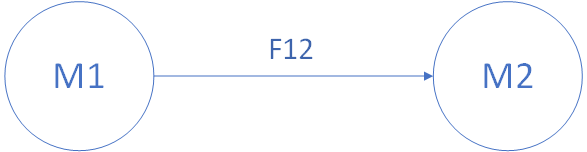
\includegraphics[width=0.8\linewidth]{grav.png}
		  \caption{Gravitation}
		  \label{fig:gravitation}
		\end{minipage}%
		\begin{minipage}{.5\textwidth}
		  \centering
		  \captionsetup{justification=centering}
		  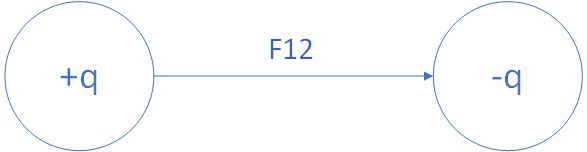
\includegraphics[width=0.8\linewidth]{el_anz.png}
		  \caption{Coulombkraft}
		  \label{fig:coulomb}
		\end{minipage}
  \end{figure}
  Vermutung: Elektronen umkreisen Atomkern wie Planeten die Sonne $\rightarrow$ nach Kepler also in einer Elipsenbahn.
  \begin{definition}$\;$\newline
    Mono: Ein \newline
    Chrom: Farbe\newline
    Monochromatisch: Einfarbig
  \end{definition}
    \subsection{Some facts}
    \begin{itemize}
	    \item Im Periodensystem nach unten werden die Atome räumlich größer
	    \item Zinn hat bis $13^\circ C$ die gleiche Kristallstruktur wie Silizium, danach baut es sich zu sogenanntem Beta-Zinn um, das dieselbe Struktur wie Metall hat.
	    \item Isotope: Bei Isotopen sind die Anzahl der Protonen gleich der Anzahl von Neutronen = der Anzahl von Elektronen. Isotope sind damit die Grundzustände von Atomen
	    \item Beschleunigt bewegte Ladungen geben Energie in Form von EM-Wellen (elektromagnetischen Wellen) ab
	    \item Größenordnung zwischen Atomen: Angström
	    \item Größenordnung im Atomkern: $10^{-15}m$
	    \item Eine Glühlampe gibt nicht monochromatisches Licht ab
	    \item Spektren vergaßter Elemente sind charackteristisch $\rightarrow$ Elemente können eindeutig erkannt werden
	    \item Frauenhofer-Linien im Sonnenspektrum durch Wasserstoff und Helium absorbiert $\rightarrow$ Elemente können aus dem Spektrum genau die Frequenzen absorbieren, die sie emittieren (Absorptionsspektrum)2
    \end{itemize}
    \newpage

	\section{29. Mai 2018: Vorlesung 7}
		\subsection{Die Bohrschen Postulate}
		\begin{itemize}
		  \item[Postulat 1: ] In den Atomen bewegen sich die Elektronen nach den Gesetzen der klassischen Mechanik auf diskreten Kreisbahnen mit den Energien $E_n$.
		  \item[Postulat 2: ] Die Bewegung des Elektrons erfolgt strahlungslos. Beim Übergang des Elektrons von einem stationären Zustand mit der Energie $E_a$ in einen stationären Zustand niedriger Energie $E_e$ wird ein Photon emittiert.
		\end{itemize}
		
		\subsection{Bohrsches Atommodell für das Wasserstoffatom}
		\begin{figure}[H] 
		  \centering
		  \captionsetup{justification=centering}
		  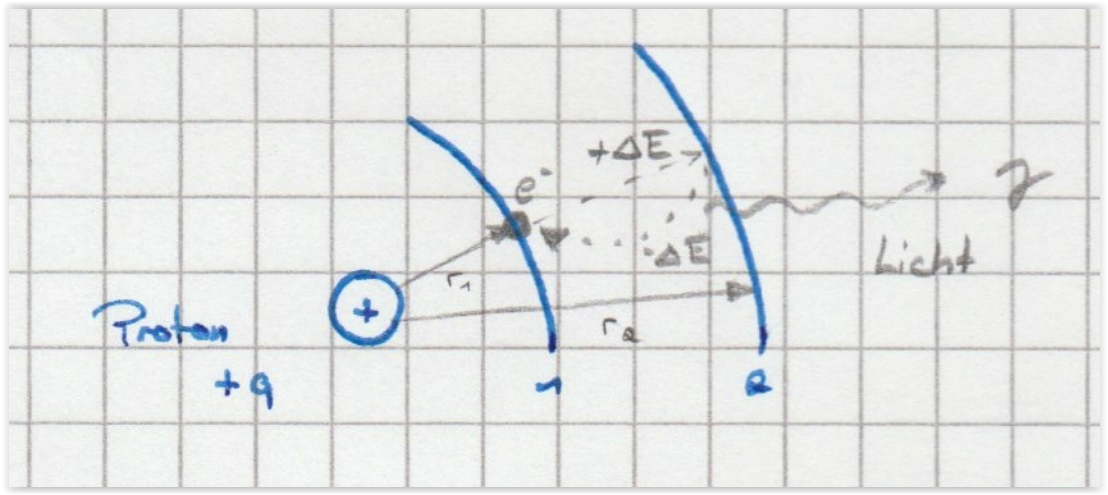
\includegraphics[width=0.6\linewidth]{atommodell_photon.png}
		  \caption{Atommodell/Bahnen \protect\cite{atom_photon}}
		  \label{fig:atommodell_photon}
		\end{figure}

    Herleitung zur Energie der Bahnradien
	  \begin{align}
	    \vv{F_c} &= \frac{1}{4 \pi \varepsilon_0} \frac{Q_1 Q_2}{|\vv{r}|^3}\vv{r} \label{eq:coulomb_2}\\ 
	    Q_1 &= +q,\qquad Q_2 = -q,\qquad \vv{r} = \vv{r_1} \nonumber \\
	    \vv{F_{c,1}} &= - \frac{1}{4 \pi \varepsilon_0} \frac{q^2}{|\vv{r_1}|^2} \frac{\vv{r_1}}{|\vv{r_2}} \quad \Rightarrow \quad |\vv{F_{c,1}}| = F_{c,1} = \frac{1}{4 \pi \varepsilon_0} \frac{q^2}{|r_1|^2} \label{eq:coulomb_3}
	  \end{align}
	  Es gilt 
	  \begin{equation}
	    E_{ges} = E_{pot} + E_{kin} = \frac{1}{2} m|\vv{v}|^2 + E_{pot} = (*)
	  \end{equation}
	  Mit $\vv{p} = m \vv{v}$ folgt:
	  \begin{equation}
	    (*) = \frac{|\vv{p}|^2}{2m} + E_{pot}
	  \end{equation}
	  \begin{figure}[H] 
		  \centering
		  \captionsetup{justification=centering}
		  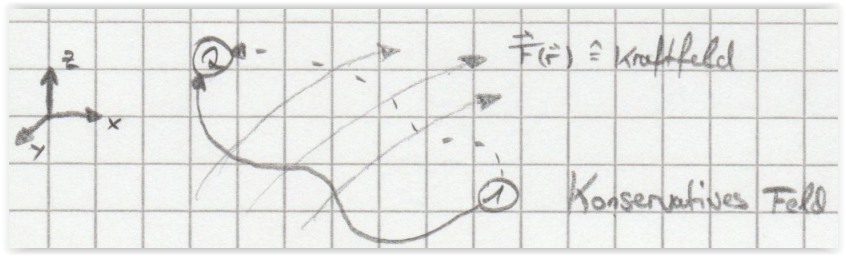
\includegraphics[width=0.6\linewidth]{bohr_kraftfeld.png}
		  \caption{Kraftwirkung auf Elektron \protect\cite{atom_photon}}
		  \label{fig:kraftwirkung_el}
		\end{figure}
		Es gilt:
		\begin{equation}
		  W = \int\limits_1^2 \vv{F}(\vv{r}) d\vv{r}
		\end{equation}
		\begin{definition}
		  Ist die nötige Arbeit unabhängig vom Weg den das Teilchen zurücklegt spricht man von einem konservativen Kraftfeld.
		\end{definition}
		D.h.:
		\begin{align}
		  &\text{Konservatives Feld } \rightarrow \oint \vv{F} (\vv{r}) d\vv{r} = 0 \\
		  &\Leftrightarrow rot \vv{F}(\vv{r}) = \vv{\nabla} \times \vv{F}(\vv{r}) = 0 \leftarrow \text{ Wirbelfreies Feld} \\ 
		  &\Leftrightarrow \vv{F}(\vv{r}) = -grad \Phi (\vv{r}) = \vv{\nabla} \phi (\vv{r})
		\end{align}
		Damit gilt:
		\begin{align}
		  \vv{F_c}(\vv{r}) = - \grad E_{pot,c} \\
		  \Rightarrow E_{pot,c} = - \frac{1}{4 \pi \varepsilon_0} \frac{Q_1 Q_2}{|\vv{r}|} \\
		  \Rightarrow E_{pot,c,1} = - \frac{1}{4 \pi \varepsilon_0} \frac{q^2}{|r_1|^2}
		\end{align}
		und somit folgt
		\begin{align}
		  \vv{F_c}(\vv{r}) = - \displaystyle\vecT{\displaystyle\frac{\diffp}{\diffp x} \\ \displaystyle\frac{\diffp}{\diffp y} \\ \displaystyle\frac{\diffp}{\diffp z}} \displaystyle E_{pot,c,1} = - \displaystyle\vecT{\displaystyle\frac{\diffp E_{pot,c,1}}{\diffp x} \\ \displaystyle\frac{\diffp E_{pot,c,1}}{\diffp y} \\ \displaystyle\frac{\diffp E_{pot,c,1}}{\diffp z}}
		\end{align}		
		Es gilt aufgrund des Vergleichs zum Planetenmodell weiter
		\begin{equation}
		  \vv{F_c} = \vv{F}_{zp} = m \vv{a}_{zp}
		\end{equation}
		Annahme: Das Elektron bewegt sich gleichförmig auf einer Kreisbahn. Dann ist
		\begin{equation}
		  \\vv{a}_{zp} = \frac{v_1^2}{r_1} 
		\end{equation}
		Wir versuchen nun die Gleichung auf die Form $1/2 mv^2$ zu bringen:
		\begin{align}
		  &\Rightarrow \frac{1}{4 \pi \varepsilon_0} \frac{q^2}{r_1^2} = m \frac{v_1^2}{r_1}\nonumber \\
		  &\Rightarrow \frac{1}{2} m v_1^2 = \frac{1}{2}\frac{1}{4 \pi \varepsilon_0} \frac{q^2}{r_1} \nonumber \\
		  &\Rightarrow E_{ges,1} = \frac{1}{2}\frac{1}{4 \pi \varepsilon_0} \frac{q^2}{r_1} - \frac{1}{4 \pi \varepsilon_0} \frac{q^2}{r_1} \nonumber \\
		  &\qquad \qquad = -\frac{1}{2} \frac{1}{4 \pi \varepsilon_0} \frac{q^2}{r_1}
		\end{align}
		Bzw. verallgemeinert
		\begin{equation}
		  E_{ges,i} = -\frac{1}{2}\frac{1}{4 \pi \varepsilon_0} \frac{q^2}{r_i}  \qquad , i = 1,2,3,...
		\end{equation}
		Beim Wechsel von einer äusseren auf eine innere Bahn wird also Energie (in Form eines Photons) frei, beim Wechsel von einer inneren auf eine äussere Bahn muss Energie aufgebracht werden.
		\begin{figure}[H] 
		  \centering
		  \captionsetup{justification=centering}
		  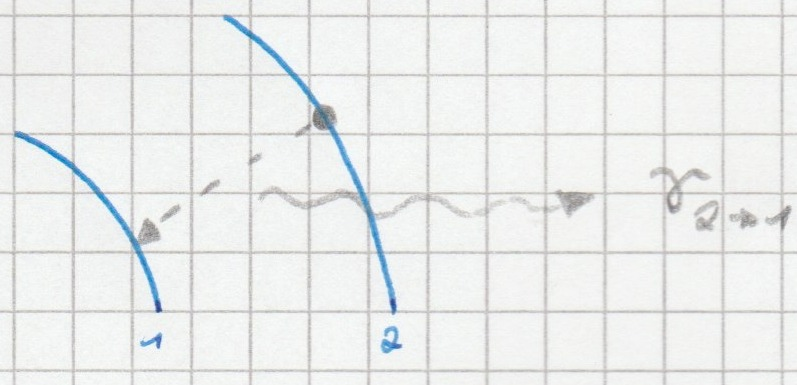
\includegraphics[width=0.4\linewidth]{atommodell_photon_2.jpeg}
		  \caption{Bahnwechsel \protect\cite{atom_photon}}
		  \label{fig:atommodell_bahnwechsel}
		\end{figure}
    \begin{align}
      E_{\gamma_{2\rightarrow 1}} &= E_{ges,2} - E_{ges,1} \nonumber \\
      &=  \frac{1}{2} \frac{1}{4 \pi \varepsilon_0} q^2 \left( \frac{1}{r_1} - \frac{1}{r_2}\right) \label{eq:bohr_energie_a}
    \end{align}    		
    Bzw. allgemein
    \begin{equation}
      E_{\gamma_{a \rightarrow e}} = \frac{1}{2} \frac{1}{4 \pi \varepsilon_0} q^2 \left( \frac{1}{r_e} - \frac{1}{r_a}\right)
    \end{equation}
    Damit allerdings sind alle Bahnradien bisher erlaubt, es liegt keine Einschränkung vor. Das würde heißen, dass das Atom das komplette Spektrum emittieren würde (also nicht diskret wäre). Es stillt sich zunächst die Frage, mit welcher Frequenz die Energie $E_{\gamma_{a \rightarrow e}}$ emittiert wird.\newline
    Idee: Nutzung der Erkentnisse zum äusseren photoelektrischen Effekt:
    \begin{equation}
      E_{\gamma_{a \rightarrow e}} \overset{?}{=} h \cdot f_{a \rightarrow e} \qquad c_0 = \lambda f \label{eq:bohr_energie_b}
    \end{equation}
		
		\subsection{Some facts}
		\begin{itemize}
		\item Systemarten
			\begin{table}[H]
				\centering
				\begin{tabular}{c c}
					Systemart & Anzahl Teilchen \\ \hline
					Mikroskopisch & Maximal 3 Teilchen \\
					Mesoskopisch & $\sim$ 100 - 1000 Teilchen\\
					Makroskopisch & $\sim$ Millionen und mehr Teilchen
				\end{tabular}
			\end{table}
			\vspace{-0.5cm}
			Bei Makroskopischen Systemen wird statistisch gearbeitet. D.h. es wird der Mittelwert des Systems untersucht um so das Problem auf ein Ein-Teilchen Problem zu reduzieren.
		\item Die Intensität einer Welle hängt vom Quadrat der Amplitude ab
		\item Die Energie einer EM-Welle hängt von der Frequenz und Intensität ab
		\item Grenzfrequenz lässt sich mit klassischer Physik nicht richtig erklären
		\item Einstein hat bei der Untersuchung des photoelektrioschen Effekts den Begriff des Photons geprägt
		\item Mehr Intensität $\Rightarrow$ mehr Photonen $\Rightarrow$ Photon $\cong h \cdot f$ $\Rightarrow$ abhängig von der Frequenz
		\end{itemize}
\newpage

	\section{05. Juni 2018: Vorlesung 8}
	\begin{definition}
	  Planksches Wirkungsquantum: 
	  \begin{align*}
	    [h]&= 1 Js = 1Nms = 1kg \frac{m}{s^2}ms =1kg \frac{m^2}{s}= 1\underbrace{kg}_{\text{Masse}} \underbrace{\frac{m}{s}}_{\text{Geschwindigkeit}} \underbrace{m}_{\text{Strecke}} \\
	    &\Rightarrow h \sim \underbrace{m \cdot v}_{p} \cdot l = p \cdot l
	  \end{align*}
	\end{definition}
	  Bekannt ist die Kombination aus Impuls und Strecke bereits vom Drehimpuls:
	  \begin{equation}
	    \vv{L} := \vv{r} \times \vv{p}
	  \end{equation}
	  Bei einer gleichförmigen Kreisbewegung steht $\vv{p}$ immer senkrecht auf $\vv{r}$ 
	  \begin{align*}
	    \Rightarrow |\vv{L}| = mvr
	  \end{align*}
	  Die Annahme liegt also Nahe, dass es sich bei dem plankschen Wirkungsquantum um einen Bahndrehimpuls handelt.\newline
	  \subsection{Quanten}
		Was ist ein Quantum? Ein Quantum ist eine Grundportion bzw. kleines Einheit. Ein Photon ist ein Energiequantm.
		\begin{table}[H]
		  \centering
		  \begin{tabular}{P{7cm} | P{7cm}}
		    Alltag & Quantenphysik \\ \hline
		    Kontinuierliche Größen & Alles besteht aus Grundquanten\newline und alles ist ein natürliches Vielfaches davon
		  \end{tabular}
		\end{table}
			\subsubsection{Erweitere Bohrsche Postulate}
			\begin{itemize}
			  \item[Postulat 1: ] In den Atomen bewegen sich die Elektronen nach den Gesetzen der klassischen Mechanik auf diskreten Kreisbahnen mit den Energien $E_n$.
			  \item[Postulat 2: ] Die Bewegung des Elektrons erfolgt strahlungslos. Beim Übergang des Elektrons von einem stationären Zustand mit der Energie $E_a$ in einen stationären Zustand niedriger Energie $E_e$ wird ein Photon der Frequenz $f = \frac{(E_a - E_e)}{h}$ emittiert, wobei $h$ das Planksche Wirkungsquantum ist.
			  \item[Postulat 3: ] Der Drehimpuls eines Elektrons in einem stationären Zustand nimmt nur diskrete Werte $2\cdot \pi \cdot m \cdot v \cdot r = n \cdot h$ an, wobei $n$ eine natürliche Zahl ist.
			\end{itemize}
		Formt man das dritte Postulat um erhält man:
		\begin{align}
		  2\cdot \pi \cdot m \cdot v \cdot r &= n \cdot h \nonumber \\
		  2 \pi p r &= n h \nonumber \\
		  \text{Bahnumfang des Elektrons} \rightarrow 2  \pi r &= \frac{nh}{p}= n \frac{h}{p}
		\end{align}
		Also sind nur solche Bahnen zulässig, die ein Vielfaches von $\frac{h}{p}$ sind. Was ist das?:
		\begin{align}
		  \text{Wellenlänge: } \lambda = \frac{h}{p} \Rightarrow \text{ Impuls: } p = \frac{h}{\lambda}
		\end{align}
		Damit ist der Bahnradius ein vielfaches der Wellenlänge. Das entspricht dem Verhalten einer stehenden Welle. Hier scheitert die klassische Mechanik, denn dabei wäre für ein massebehaftetes Teilchen keine Wellenlänge vorgesehen ist.
		\begin{definition}
		  Dirac-Konstante:
		  \begin{equation}
		    \hbar = \frac{h}{2 \pi}
		  \end{equation}
		\end{definition}
		\begin{align*}
		  mvr &= n \frac{h}{2\pi} = n \hbar \\
		  \Rightarrow r_{n} &= n^2 \hbar ^2 4 \pi \varepsilon_0 \frac{1}{mq^2}\qquad ,n \in \N_{\backslash \lbrace 0 \rbrace}\\
		  \Rightarrow r_n &= n^2 r_1 \\
		  r_1 &=  \hbar ^2 4 \pi \varepsilon_0 \frac{1}{mq^2} = 0,0529nm
		\end{align*}
		$r_1$ wird Bohrscher Radius genannt. Im Wasserstoffatom ist es der kleinste zulässige Radius.
		Setzt man dies in \eqref{eq:bohr_energie_a} ein und stellt \eqref{eq:bohr_energie_b} nach der Frequenz um, erhält man
		\begin{align}
		  f_{\gamma_{a \rightarrow b}} &= \frac{E_{\gamma_{a \rightarrow b}}}{h}=\frac{1}{2} \frac{1}{4 \pi \varepsilon_0} \frac{q^2}{h}\left( \frac{mq^2}{n_e^2 4 \pi \varepsilon_0 \hbar^2} - \frac{mq^2}{n_a^2 4 \pi \varepsilon_0 \hbar^2}\right) \nonumber \\
		  &= \frac{1}{2}\frac{1}{4\cancel{\pi}\varepsilon_0} \frac{q^2}{h} \frac{mq^2}{\cancel{4} \cancel{\pi} \varepsilon_0 \frac{h^2}{(\cancel{2} \cancel{\pi})^2}} \left( \frac{1}{n_e^2} - \frac{1}{n_a^2}\right)= \frac{mq^4}{8\varepsilon_0^2 8 \pi^3 \frac{h^3}{8 \pi^3}}\left( \frac{1}{n_e^2} - \frac{1}{n_a^2}\right)  \nonumber \\
		  &= \frac{mq^4}{(4 \pi \hbar)^3 \varepsilon_0^2}\left( \frac{1}{n_e^2} - \frac{1}{n_a^2}\right)
		\end{align}
		Die so berechneten Spektrallinien stimmen exakt mit denen von  Wasserstoff überein. Damit ist es recht wahrscheinlich, dass die Rechnung richtig ist. Je schwerer die Atome werden, desto weniger exakt ist das Modell allerdings.
		Im Kristall kommen die Atome mikroskopisch nah zusammen. Dabei fächern sich die energetischen Zustände zu Energiebändern auf. Die Energiedifferenzen zwischen den Radien geben dabei die Bandlücken an.
		\subsection{Dipolmoment}
		\begin{figure}[H] 
		  \centering
		  \captionsetup{justification=centering}
		  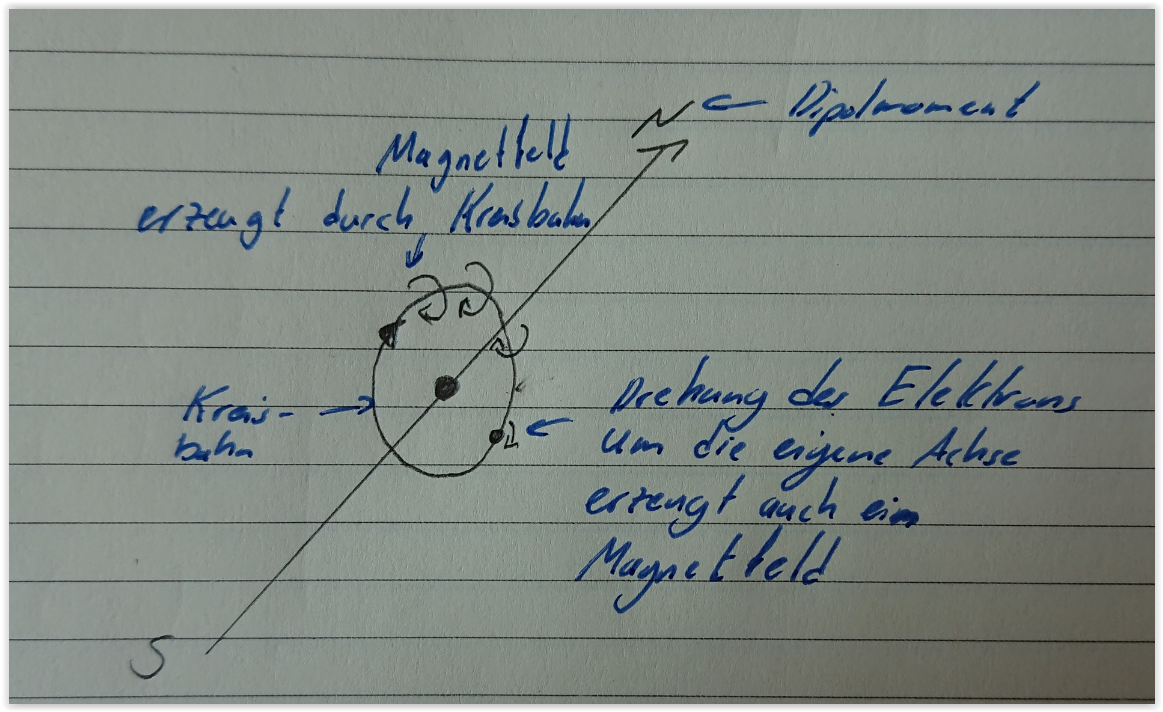
\includegraphics[width=0.7\linewidth]{dipolmoment_el.png}
		  \caption{Dipolmoment eines Elektrons}
		  \label{fig:atommodell_Dipolmoment}
		\end{figure}
		Die Bewegung des Elektrons entlang der Kreisbahn erzeugt ein Magnetfeld, die Drehung um die eigene Achse (Spin) erzeugt wiederrum auch ein eigenes Magnetfeld. Zusätzlich zu den Bahnradien gibt es nach Somemrfeld $n-1$ stabile Ellipsen in denen sich Elektronen befinden können. Dabei spricht man von Energieschalen. 
		\subsection{Some facts}
		\begin{itemize}
		  \item PTB = \ul{P}hysikalisch \ul{T}echnische \ul{B}undesanstalt, im Prinzip ein Eichinstitut
		  \item Pauliprinzip: Jeder Zustand (auch einzelne Spins) ist entweder frei oder durch nur ein Elektron besetzbar
		\end{itemize}
\newpage

	\section{26. Juni 2018a: Vorlesung 9a}
		\subsection{Metalle und metallische Leitfähigkeit}
		Metalle zeichnen sich insbesonderen durch
		\begin{itemize}
		  \item Hohe elektrische Leitfähigkeit die mit steigender Temperatur abnimmt
		  \item Hohe Wärmeleitfähigkeit
		  \item Duktilität (Verformbarkeit, Schmiedbarkeit)
		  \item Metallischer Glanz (Spiegelglanz)
		\end{itemize}
		aus.
		Weiterhin leiten Metalle elektromagnetische Wellen nicht.
		
		\subsection{Bandstruktur}
		Zur kompletten Beschreibung der Bandstruktur würde man eine Dimension für die Energie, drei für dem Impuls und drei für den Ort benötigen. Zur Darstellung unterteilt man oft in den Impuls- sowie den Ortsraum.
		\begin{figure}[H] 
		\centering
		\begin{minipage}{.5\textwidth}
		  \centering
		  \captionsetup{justification=centering}
		  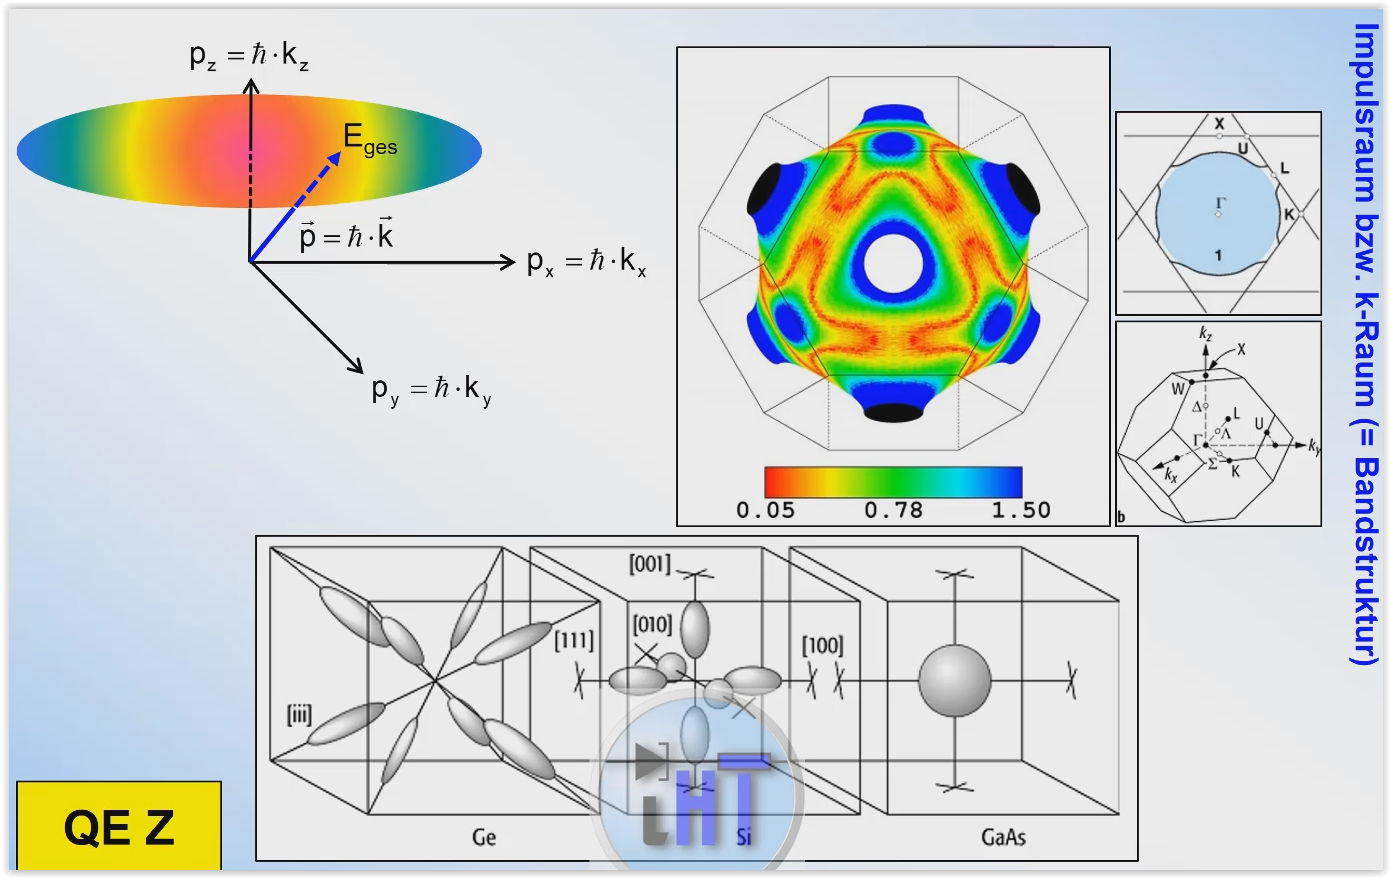
\includegraphics[width=0.8\linewidth]{bandstruktur_impulsraum.png}
		  \caption{Impulsraum \protect\cite{MIKRO2}}
		  \label{fig:bandstr_impulsraum}
		\end{minipage}%
		\begin{minipage}{.5\textwidth}
		  \centering
		  \captionsetup{justification=centering}
		  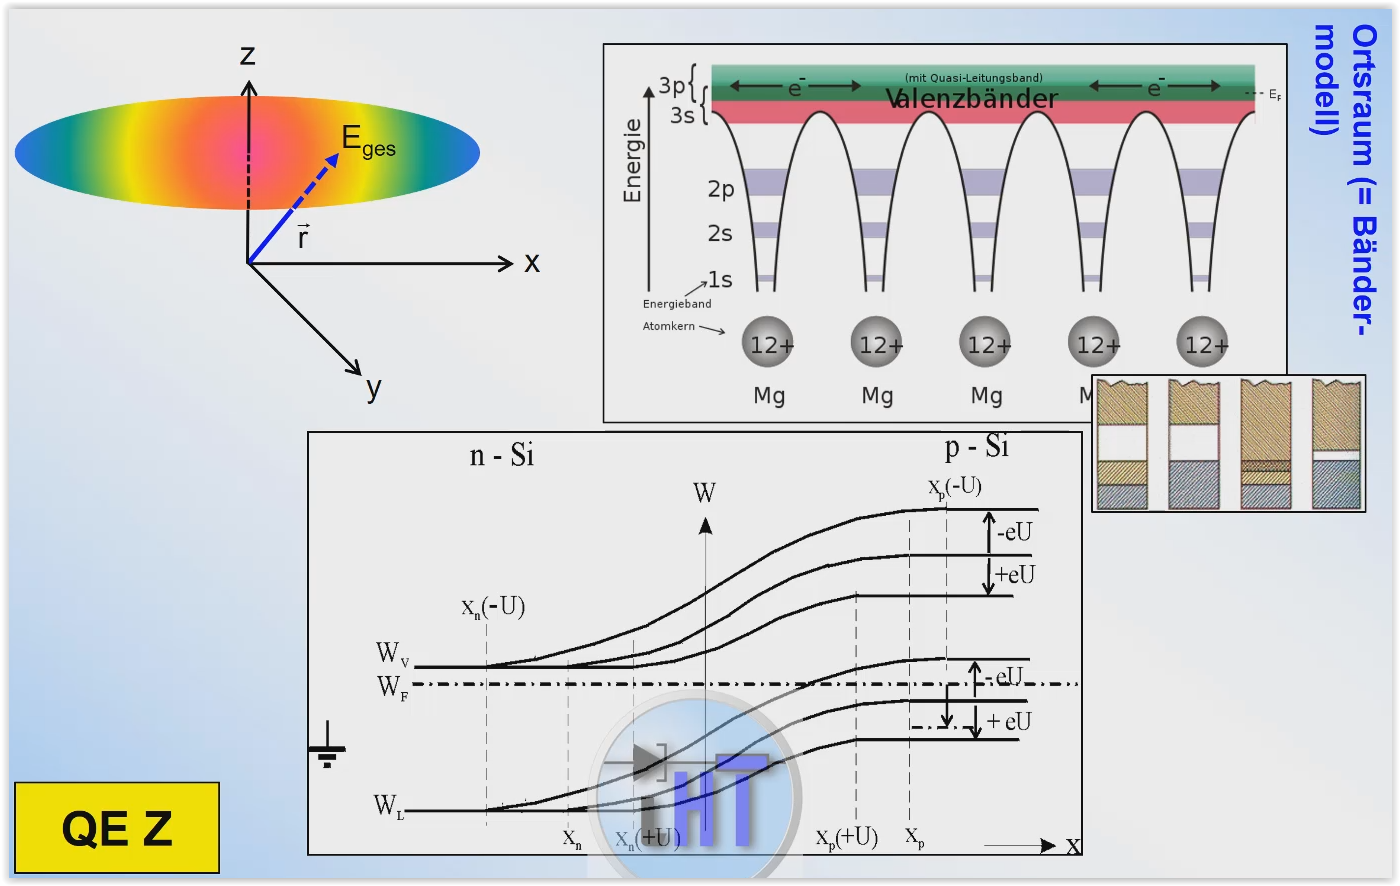
\includegraphics[width=0.8\linewidth]{bandstruktur_ortsraum.png}
		  \caption{Ortsraum \protect\cite{MIKRO2}}
		  \label{fig:bandstr_ortsraum}
		\end{minipage}
  \end{figure}
  
		\subsection{Metallische Bindung}
		Bei metallischer Bindung entsteht ein sogenanntes Fermi-Gas. Im statistischen Mittel gibt jedes Atom im Metall 1-2 Elektronen in einen sogenannten Fermi-See bzw. in das sogenannte Fermi-Gas ab. Aufgrund des Verhalten eines Gases lassen sich thermodynamische Prinzipien anwenden. Die Metalle halten durch die Coulombkraft zusammen. Das Metal besteht im Prinzip aus positiv geladenen Metallionenrümpfen die von einem negativen Fermi-See umspült sind.
		
    Zunächst der Versuch der Illustrierung einer Bandstruktur in einem Universum in dem es nur ein einzelnes Elektron gibt.
    \begin{equation}
      E_{ges} = E_{pot} + E_{kin}   
    \end{equation}       
    Die potentielle Energie wird zu $0$, da es keine weiteren Objekte gibt die eine Kraftwechselwirkung mit dem Elektron haben. Daher gilt $E_{ges} = E_{kin}$. Bei diesem Gedankenexperiment sind alle Energien positiv da es keine weiteren Teilchen und somit keine Bindungen gibt. Also gilt:
    \begin{align*}
      0 \leq E_{ges} = E_{kin} < E_{max} 
    \end{align*}
    Mit
    \begin{align*}
      E_{kin} &= \frac{1}{2}m |\vv{v}|^2 = \frac{|\vv{p}|^2}{2m}\\
      \vv{p} &= \vecT{p_x \\ p_y \\ p_z} \Rightarrow E_{kin} = \frac{1}{2m} \left( \sqrt{p_x^2 + p_y^2 + p_z^2}\right)^2 = \frac{1}{2m} \left(p_x^2 + p_y^2 + p_z^2\right)\\
      \Leftrightarrow 2m E_{kin} &= p_x^2 + p_y^2 + p_z^2 \\
      \Rightarrow konst. &= p_x^2 + p_y^2 + p_z^2
    \end{align*}
    Hierbei handelt es sich um eine Kugelgleichung. 
    \begin{figure}[H] 
		  \centering
		  \captionsetup{justification=centering}
		  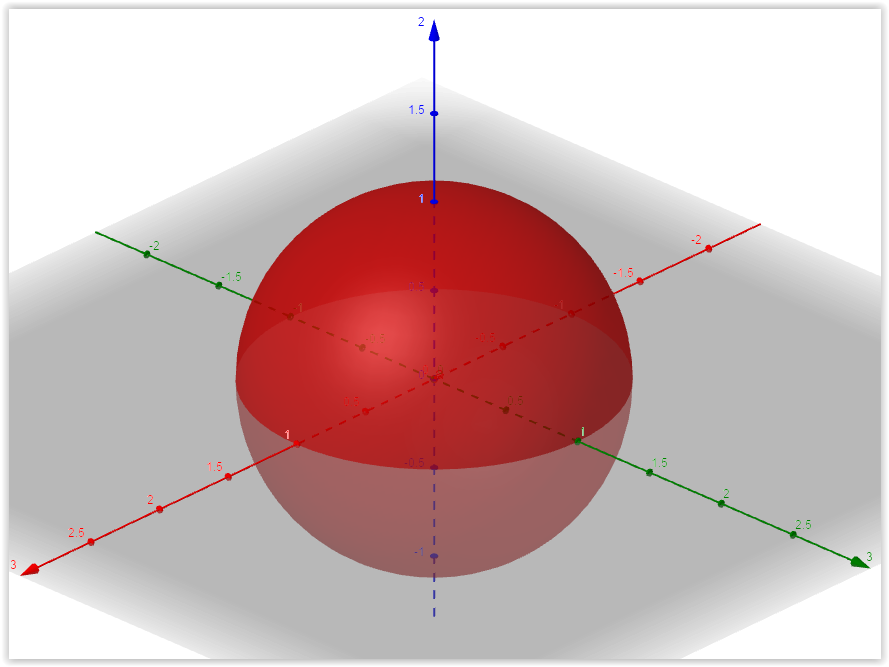
\includegraphics[width=0.4\linewidth]{kugel.png}
		  \caption{Kugelschale}
		  \label{fig:kugelschale}
		\end{figure}
		D.h. die Lösungsmenge sind alle Vektoren die auf diese Kugelschale zeigen. Damit ist unklar in welche Richtung sich das Elektron bewegen wird. Es ist 
		Übersichtlicher ist das Orstmodell. Da das Bohrsche Atommodell zweidimensional ist bleibt im Karthesischen System noch eine Dimension frei, die mit der Energie genutzt werden kann. So lässt wich die gesamte potentielle Energie die ein Teilchen in einer Ebene von positiv geladenen Metallionen haben kann.
		Dabei gilt:
		\begin{align}
		  E_{pot,kristall} &= \sum\limits_i E_{pot,i} \\
		  \text{mit} \nonumber \\
		  E_{pot,i} &= - \frac{1}{4 \pi \varepsilon_0 \varepsilon_{rel}} \frac{Z q^2}{\sqrt{(x-x_i)^2+(y-y_i)^2+(z-z_i)^2}}
		\end{align}
		\begin{figure}[H] 
		\centering
		\begin{minipage}{.5\textwidth}
		  \centering
		  \captionsetup{justification=centering}
		  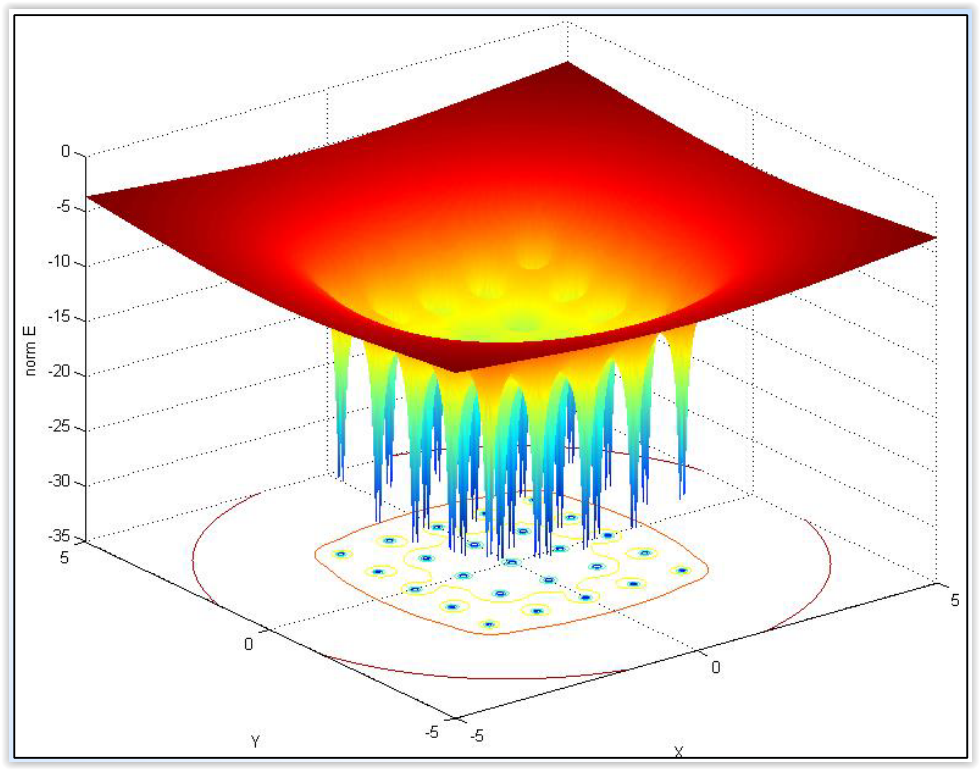
\includegraphics[width=0.7\linewidth]{potentiale_2d.png}
		  \caption{Potentielle Energie im Ortsraum 2D \protect\cite{MIKRO2}}
		  \label{fig:ortsraum_pot_2d}
		\end{minipage}%
		\begin{minipage}{.5\textwidth}
		  \centering
		  \captionsetup{justification=centering}
		  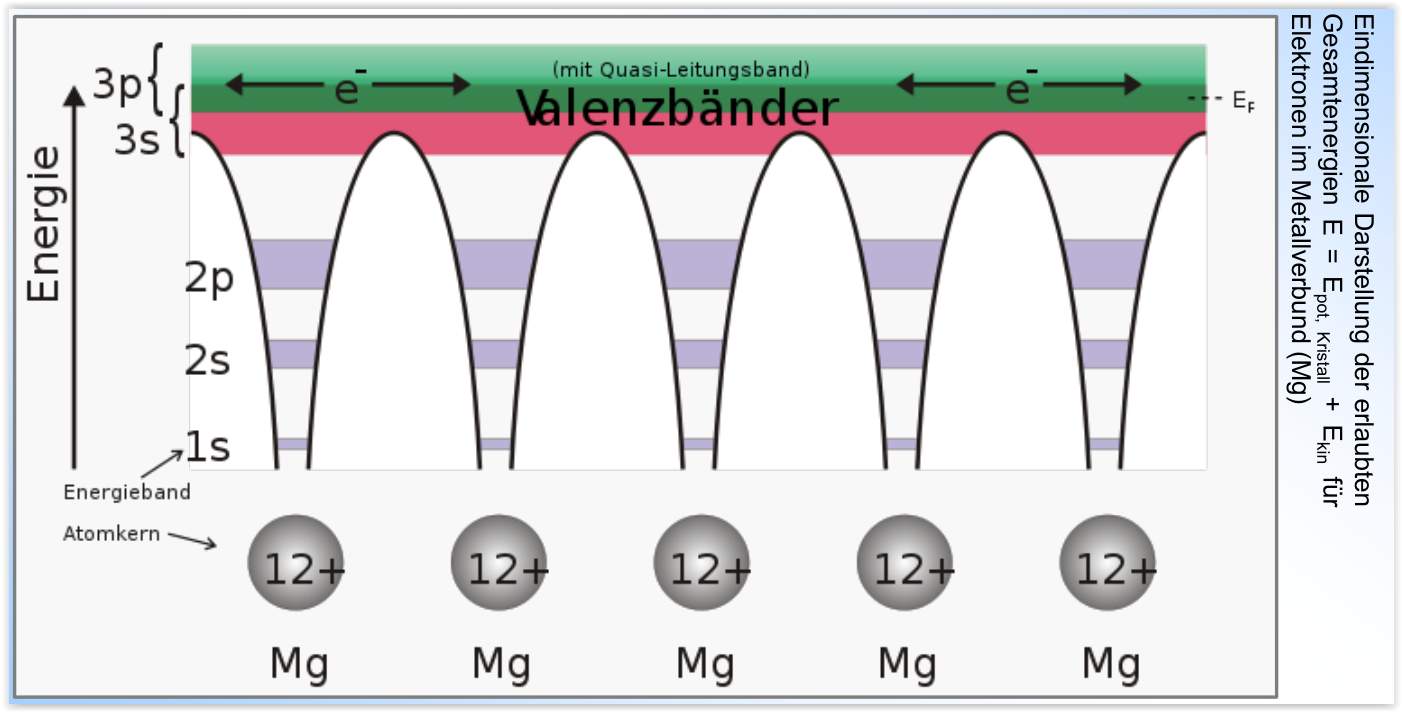
\includegraphics[width=1.1\linewidth]{potentiale_1d.png}
		  \caption{Potentielle Energie im Ortsraum 1D \protect\cite{MIKRO2}}
		  \label{fig:ortsraum_pot_1d}
		\end{minipage}
  \end{figure}
  Hat das Teilchen genügend Energie wird es$\;$\grqq über die Löcher springen\grqq$\;$und nicht in die Trichter fallen (vgl. Kugel über Trichter). Betrachtet man den Querschnitt von \eqref{fig:ortsraum_pot_2d} erhält man \eqref{fig:ortsraum_pot_1d}. Ist ein Teilchen mal in einen Trichter gefallen wird es ohne Zugabe von Energie nicht mehr herauskommen.
  
    \subsection{Ohmsches Gesetz}
    Es gilt
    \begin{align}
      \vv{j} &= \sigma \vv{\varepsilon} \\
      U &= RI \\
      \sigma &= q n \mu
    \end{align}
    Mit $n$ als Ladungsträgerdichte und $\mu$ als Ladungsträgerbeweglichkeit. Um ohmsches Verhalten (also eine lineare Strom/Spannungs Kennlinie) zu erhalten, muss überall die gleiche Ladungsträgerkonzentration vorhanden sein und es muss sich eine für alle gleiche Driftgeschwindigkeit ergeben, also 
    \begin{align*}
      n &= konst.\\
      \vv{v}_D &= konst.
    \end{align*}
    Damit lässt sich die Kirchhoffsche Regel, die mit 
    \begin{equation}
      \sum\limits_i I_i = 0
    \end{equation}
    gegeben ist, erklären. Da die Ladungsträgerkonzentration überall konstant sein muss kann sich die Konzentration im Knoten nicht erhöhen. In einem Metall verhält sich das Elektronensystem also wie eine inkompressible Flüssigkeit.
    
    Hierzu betrachten wir die Kontinuitätsgleichung in differentieller Form
    \begin{equation}
      \frac{\diffp \varrho}{\diffp t}+ \vv{\nabla} \vv{j} = 0 \label{eq:kontin_diff}
    \end{equation}
    Die Gleichung wird in integrieller Form für große Volumina und in differentieller Form für infinitesimal kleine Volumina genutzt. Die Divergenz auf $\vv{j}$ angewendet ist hierbei die Betrachtung der Differenz dessen was aus dem Knoten heraus und hinein fließt. Dies kann negativ, positiv oder Null sein.\newline
    \begin{table}[H]
	    \centering
	    \begin{tabular}{c | c}
		    Positiv & Quelle \\
		    Negativ & Senke \\
		    Null & Neutral
	    \end{tabular}
    \end{table}
    Die Kirchhoffsche Regel ist ein Spezialfall, der sich nur ergibt wenn die Divergenz auf $\vv{j}$ angewandt Null ist, denn dabei muss auch der erste Teil der Summe Null sein.
    \subsection{Homogen dotiertes Silizium}
    Ein so dotierter Halbleiter ergibt einen linearen U/I Zusammenhang. Ein n-dotierter Halbleiter hat dabei eine steilere Steigung als der p-dotierte Halbleiter. Man würde erwarten das beim Zusammenführen beider Halbleiter ein Ohmsches Verhalten vorliegt, also wieder eine Gerade heraus kommt. Dem ist aber nicht so, da sich dabei eine Diodenkennlinie gibt. Das erklärt sich dadurch, dass die Konzentrationen von Löchern und Elektronen in beiden Halbleitern extrem unterschiedlich sind und somit ein sehr hoher Konzentrationsgradient vorhanden ist. Dadurch unterscheidet es sich deutlich von klassisch ohmschen Widerständen.
    \begin{figure}[H] 
		\centering
		\begin{minipage}{.5\textwidth}
		  \centering
		  \captionsetup{justification=centering}
		  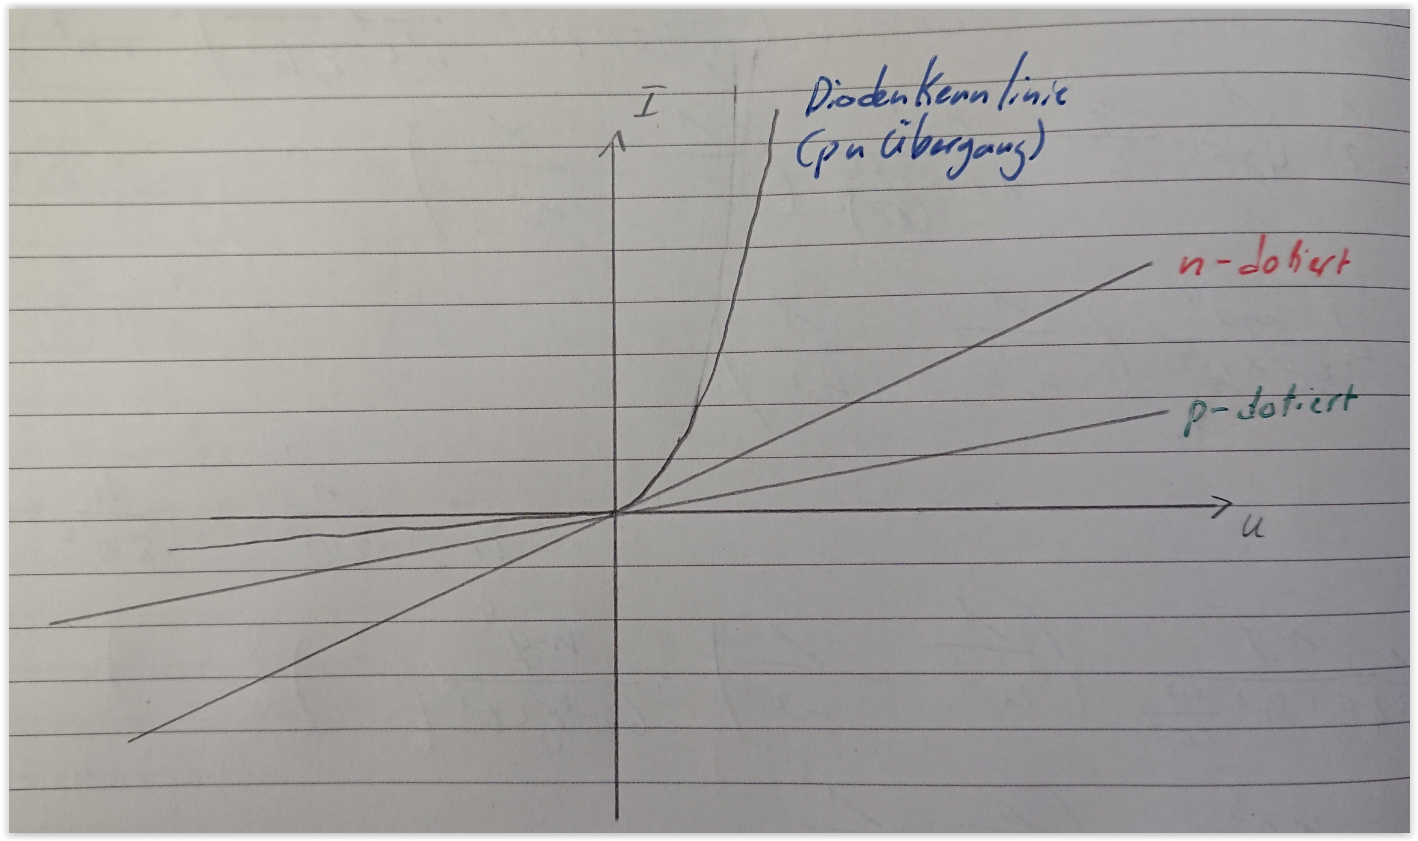
\includegraphics[width=0.9\linewidth]{hom_hl_kurven.png}
		  \caption{Homogene Halbleiter U/I Kurve}
		  \label{fig:hom_hl_kurven}
		\end{minipage}%
		\begin{minipage}{.5\textwidth}
		  \centering
		  \captionsetup{justification=centering}
		  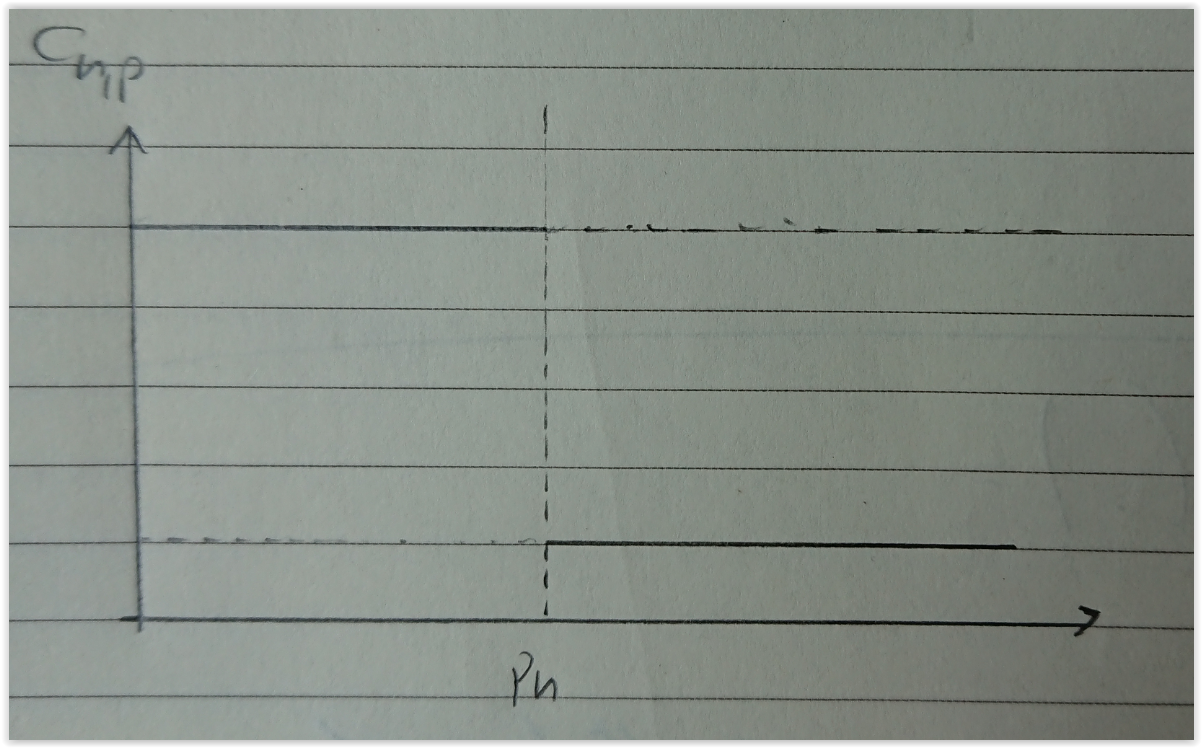
\includegraphics[width=0.85\linewidth]{hom_hl_konz.png}
		  \caption{Homogene Halbleiter Konzentration}
		  \label{fig:hom_hl_konz}
		\end{minipage}
  \end{figure}
  Dabei gilt:
  \begin{align}
    n \approx N_D \qquad p \approx N_A\\
    n = \frac{n_i^2}{N_A} \qquad p = \frac{n_i^ 2}{N_D}
  \end{align}
		\subsection{Some facts}
			\begin{itemize}
			  \item Elemente gehen nur solche chemische Verbindungen ein, dass sie möglichst in Edelgaskonfiguration kommen, also abgeschlossene Außenschalen haben
			  \item Im Periodensystem stehen Metalle meistens in sogenannten Übergangsgruppen bzw. Nebengruppen. Hier ist es schwierig zu sagen ob ein Element Elektronen aufnehmen oder abnehmen sollte um Edelgaskonfiguration zu erreichen
			  \item In Materie befinden sich ca. $10^{23} cm^{-3}$ Atome, gibt nun jedes dieser Atome 1-2 Elektronen in den Fermi-See abgibt erhalten wir ca. $1-2 \cdot 10^{23} cm^{-3}$ Elektronen $\Rightarrow$ sehr hohe Leitfähigkeit
			  \item Zu 99\% besteht Materie aus nichts
			  \item Komplette Bandstruktur wäre ein 7D Bild
			  \item Metalle werden nach Dichte klassifiziert (Leicht- und Schwermetall)
			  \item In einem Metall ist der letzte bei $T = 0K$ noch besetzte energetische Zustand das Fermi-Niveau
			  \item Die Elektronen die bei einem Metall hauptsächlich für die Leitfähigkeit eine Rolle spielen sind die Nahe des Fermi-Niveaus, da dort die Hauptmasse der Elektronen ist
			\end{itemize}
\newpage

	\section{26. Juni 2018b: Vorlesung 9b}
	\subsection{PN-Übergang}
	In einem ohmschen Knoten gilt $\diverg = 0$, d.h. $n = konst.$. Die Diffusion wird durch die Fickschen Gesetze beschrieben. Das erste Ficksche Gesetzt besagt, bei Vorhandensein eines Konzentrationsgradienten kommt es zu einem Diffusionsstrom, der von der höheren zur niedrigeren Konzentration fließt bis sämtliche Konzentrationsunterschiede ausgeglichen sind. Bei dem in \eqref{fig:hom_hl_konz} illustrierten Fall, würde es zu einem Diffusionsstrom kommen, da gigantische Konzentrationsunterschiede vorliegen. Der Ladungszustand des Gesamtsystems bleibt dabei beim Kontakt beider Materialien neutral. Der Diffusionsstrom nach Kontakt setzt sich dabei aus zwei Teilen zusammen. Zum einen ein Elektronenstrom von der N-Typ zur P-Typ Seite und ein genau entgegengesetzt gerichteter Löcherstrom. \newline
	Setzt man ein infinitesimal kleines Volumen direkt an den PN Übergang benötigt man zwei Kontinuitätsgleichungen zur korrekten Beschreibung. Eine für Elektronen und eine für Löcher. Dabei wird klar, dass das selbe Volumen sowohl eine Quelle als auch eine Senke sein kann (je für Elektronen und Löcher). Hier im Beispiel ist das Volumen eine Quelle für Löcher und eine Senke für Elektronen. Betrachtet man also die Divergenz des Löcherstroms stellt sich heraus, dass es eine positive Divergenz ist (es fließen mehr Löcher heraus als hinein). Damit weiterhin \eqref{eq:kontin_diff} war bleibt muss damit die Dichte der Löcher im Volumen negativ sein also physikalisch abnehmen. 
  \begin{figure}[H]
	  \centering
	  \captionsetup{justification=centering}
	  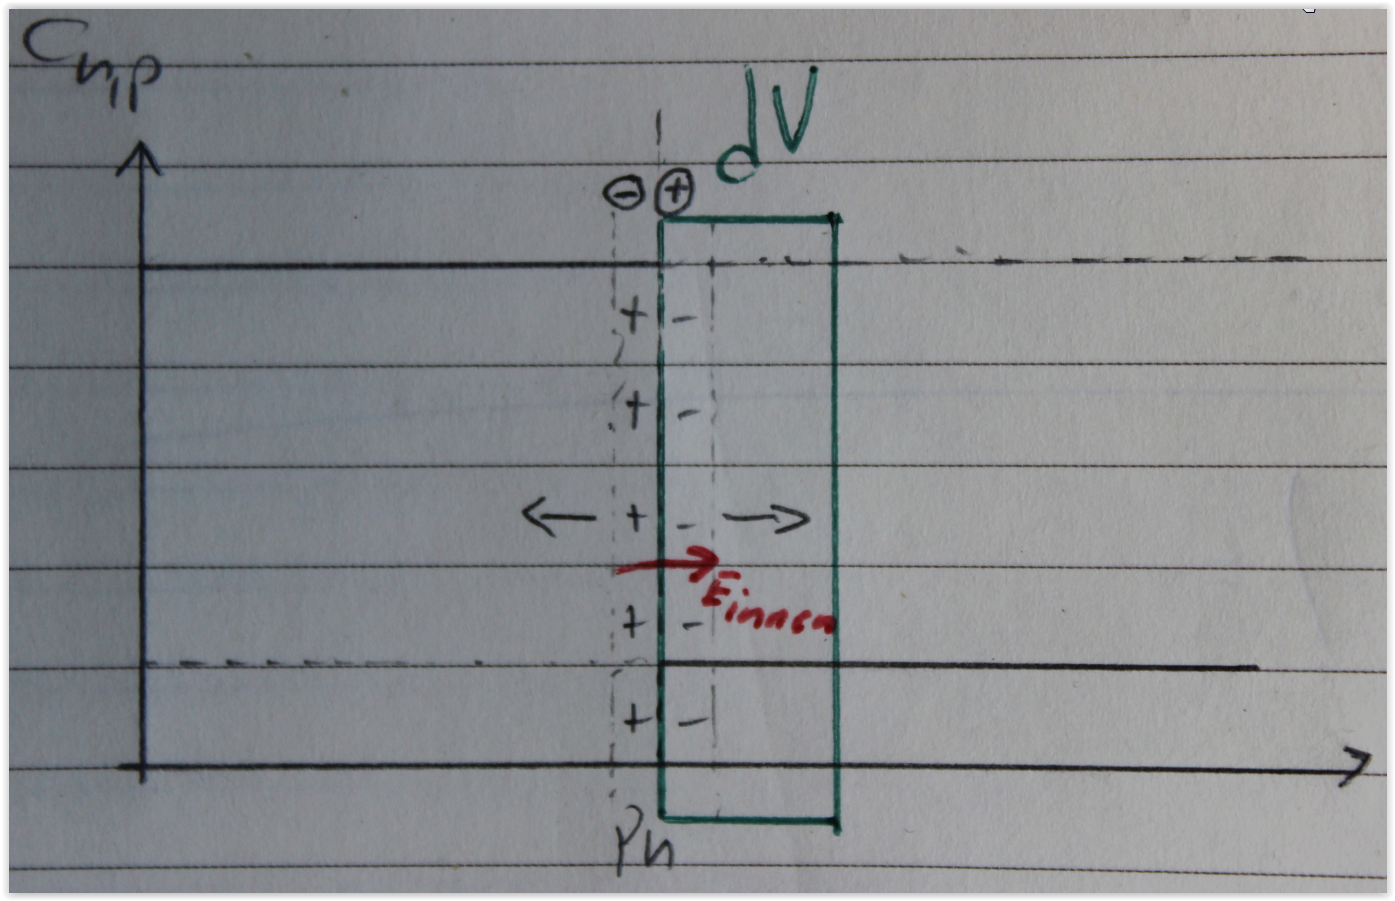
\includegraphics[width=0.6\linewidth]{hom_hl_rlz.png}
	  \caption{Homogene Halbleiter Raumladungszone}
	  \label{fig:hom_hl_rlz}
	\end{figure}
  Die Schlussfolgerung daraus ist wiederum, dass sich auf der einen Seite eine positive Überschussladung generiert (und zwar mit jedem Elektron, das hier im Beispiel von links nach rechts diffundiert, denn so wird im linken HL eine positive Ladung nicht mehr kompensiert). Dasselbe passiert durch das diffundieren der Löcher von rechts nach links, sodass sich eine negative Überschussladung generiert. Dadurch baut sich ein elektrisches Feld auf, dass von $+$ nach $-$ zeigt. Während die Diffusion weiter abläuft steigt das elektrische Feld immer weiter an. Dieses elektrische Feld wirkt dabei genau entgegengesetzt der Diffusion. Diffundieren im Beispiel Elektronen nach rechts wirkt gleichzeitig durch das innere elektrische Feld eine Kraft, die versucht die Elektronen zur positiven Seite der RLZ (Raumladungszone) zu beschleunigen. Würde dieses elektrische Feld nicht entstehen, würde die Diffusion ablaufen bis der Konzentrationsgradient Null wäre. \newline
  Nach der Schottkyschen Parabelnäherung gibt es in der Raumladungszone keine freien Ladungsträger, da sie durch das elektrische Feld direkt heraus beschleunigt werden würden. Nach einiger Zeit ist das elektrische Feld so groß, dass die Diffusion nicht mehr ablaufen kann. Der Gradient ist zwar weiterhin ungleich Null, dennoch wird die Diffusion aufgehalten obwohl weiterhin Diffusionsdruck vorherrscht. 
  Betrachten wir \eqref{fig:hom_hl_kurven} erneut erkennt man, dass der Strom in Vorwärtsrichtung um Größenordnungen größer als der in Rückwärtsrichtung ist. In Vorwärtsrichtung ist das äussere elektrische Feld dem inneren gerade entgegengesetzt gerichtet. Damit wird das innere elektrische Feld geschwächt, die RLZ wird kleiner und das innere el. Feld behindert den Diffusionsstrom weniger. Weiterhin ist die Leitfähigkeit direkt proportional zur Anzahl der strömenden Ladungsträger. Wurde zum Beispiel mit $10^{17}cm^{-3}$ auf beiden Seiten dotiert dotiert dann werden so in Vorwärtsrichtung jeweils $10^{17}cm^{-3}$ Löcher und Elektronen in jeweils die andere Seite transportiert $\Rightarrow$ großer Strom. \newline
  In Rückwärtsrichtung wird das innere elektrische Feld gestärkt und die Raumladungszone wird immer größer. Dadurch wird der Diffusionsstrom immer stärker behindert. Der dabei dann noch vorhandene Strom wird Rekombinations- und Generationsmechanismen die immer in einem Halbleiter ablaufen ($10^{10} cm^{-3}$ Elektronen/Löcherpaare). Generiert sich innerhalb der RLZ ein Elektronen/Lochpaar, wird das Paar durch das elektrische Feld sofort voneinander getrannt und in entgegengesetzte Richtungen weggesaugt. \newline
  Stellt man sich nun die Frage, wodurch in \eqref{fig:hom_hl_kurven} das exponentielle Wachstum entsteht betrachtet man am besten den PN-Übergang und die Bandverbiegung.
  \begin{figure}[H]
	  \centering
	  \captionsetup{justification=centering}
	  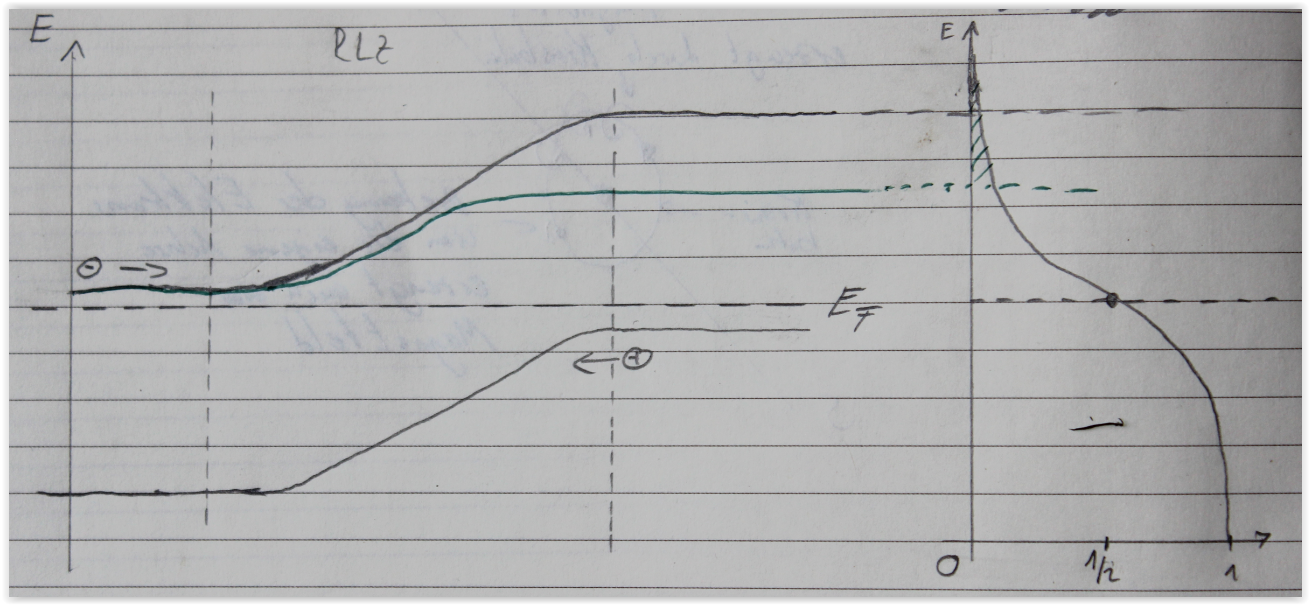
\includegraphics[width=0.6\linewidth]{hom_hl_pn.png}
	  \caption{Homogene Halbleiter Bandverbiegung}
	  \label{fig:hom_hl_pn}
	\end{figure}
	Betrachtet man das eingezeichnete Loch bzw. Elektron stellt man fest, dass zuerst Energie zugeführt werden muss damit die $\;$ \grqq Barriere \grqq $\;$ in Form der Bandverbiegung überwunden werden kann. Legt man nun ein elektrisches Feld in Vorwärtsrichtung an wird die Raumladungszone immer kleiner. Da das innere elektrische Feld ursächlich für die Bandverbiegung ist wird entsprechend auch die Bandverbiegung immer kleiner und somit muss den Elektronen/Löchern weniger Energie zugeführt werden, damit Sie den PN-Übergang passieren können. Betrachtet man dazu die Fermi-Verteilung wird klar, dass direkt am Anfang direkt ein kleiner Strom fließt, da es einige wenige Elektronen gibt, die hochenergetisch genug sind um die Barriere zu überwinden. Je geringer die Bandverbiegung nun wird (in grün eingezeichnet), desto höher wird die Besetzungswahrscheinlichkeit nach der Fermi-Verteilung. Diese Wahrscheinlichkeit nimm exponentiell zu. Damit nimmt auch der Stromfluss entsprechend der Diodenkennlinie exponentiell zu.
	
	\subsection{Schottky-Kontakt}
	\subsubsection{Metall/n-Typ Halbleiter Übergang}
	Im Metall ist typischerweise ein Fermi-See aus frei beweglichen Elektronen vorhanden. Im N-Typ Halbleiter haben die Donator-Atome bei RTP ihr zusätzliches Elektron abgegeben. Diese Elektronen sind zunächst genauso frei beweglich die wie Elektronen im Fermi-See im Metall. Vor dem Kontakt beider Materialien sind beide jeweils in sich elektrisch völlig neutral. Im Metall sind $\sim 1-2 \cdot 10^{23} cm^{-3}$ freie Ladungsträger vorhanden, im Halbleiter entspricht die Elektronenkonzentration dann ungefähr der Donator- bzw. Dotierkonzentration, also z.B. $\sim 10^{18} cm^{-3}$. Somit wäre die erste Vermutung, dass ein Konzentrationsgradient vorliegt und das System bei Kontakt versucht das Gefälle auszugleichen. Damit müssten vom Metall zum Halbleiter Elektronen fließen. Dem ist aber nicht so. Tatsächlich fließen vom Metall in den Halbleiter Elektronen. Für die Wahl des Metalls gibt es grundsätzlich drei Möglichkeiten. Das Fermi-Niveau des Metalls könnte unterhalb dem des Halbleiters, oberhalb oder gleich sein. Technisch relevant ist vor allem der Fall, in dem das Fermi Niveau des Metalls unterhalb dem des Halbleiters liegt. In Diesem Fall befindet sich der Hauptteil der Elektronen im Metall auf der Höhe der Bandlücke im Halbleiter. Es besteht dann zwar ein hoher diffusiver Druck von Seiten des Metalls, es kann aber keine Diffusion stattfinden. Die einzigen Elektronen die Tatsächlich wandern können sind die, die auf Höhe des Leitungsbands des Halbleiters liegen. Dort sind aber im Metall entsprechend der Fermi-Verteilung nur sehr wenige Elektronen vorhanden. Dagegen sind im Halbleiter entsprechend der Dotierung $\sim 10^{18} cm^{-3}$ vorhanden. Dementsprechend ist ein Konzentrationsgradient vorhanden und es kommt zu einer Diffusion vom Halbleiter ins Metall. Das Metall ist allerdings im Verhalten wie eine inkompressible Flüssigkeit. Daher können nicht einfach mehr Elektronen in das Metall gebracht werden. Die aus dem Halbleiter diffundierenden Elektronen befinden sich wie in \eqref{fig:schottky_m-n_diff} zu sehen ist direkt an der Grenzfläche. Dies verhält sich wie eine Flächenladung beim Kondensator. Somit bildet sich eine Raumladungszone an der Kontaktfläche zwischen Metall und N-Typ Halbleiter (wobei die positive RLZ räumlich stark ausgedehnt ist), da die Donatoren als einfach positive Ionen im Halbleiter zurückbleiben und die diffundierten an der Grenzfläche zum Metall als negative RLZ verbleiben. Erhöht man die angelegte Spannung über das interne Feld hinaus kommt zum vorhandenen Diffusionsstrom noch ein Driftstrom hinzu. 
	\begin{figure}[H] 
		\centering
		\begin{minipage}{.5\textwidth}
		  \centering
		  \captionsetup{justification=centering}
		  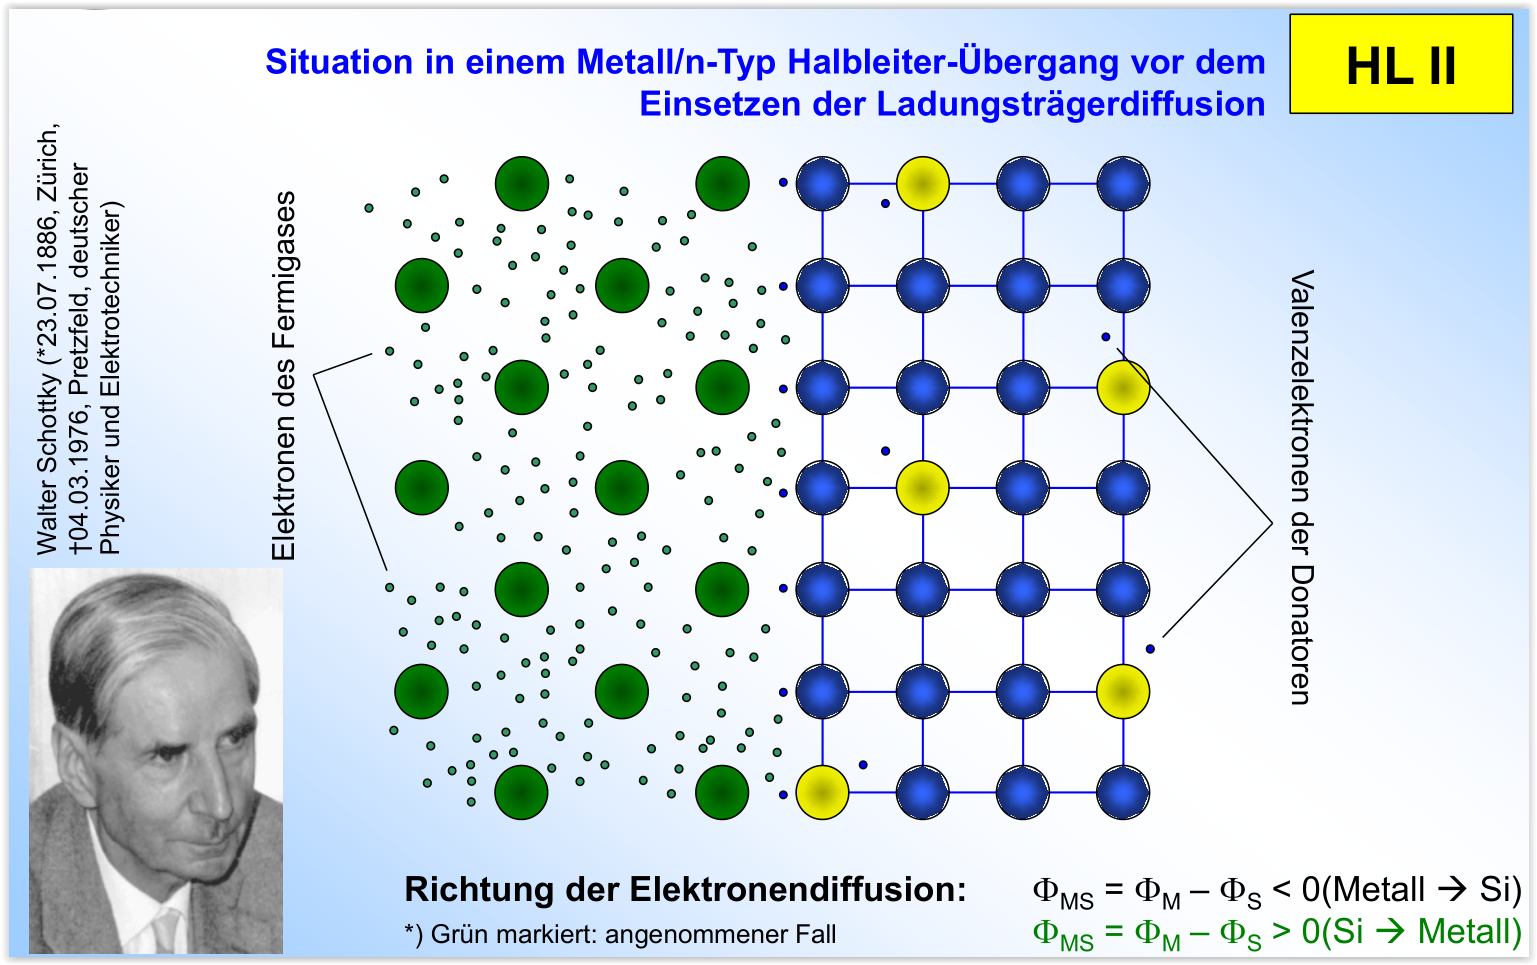
\includegraphics[width=0.95\linewidth]{schottky_m-n_vorher.png}
		  \caption{Schottky Kontakt Metall/n-Typ vor der Diffusion \protect\cite{MIKRO2}}
		  \label{fig:schottky_m-n}
		\end{minipage}%
		\begin{minipage}{.5\textwidth}
		  \centering
		  \captionsetup{justification=centering}
		  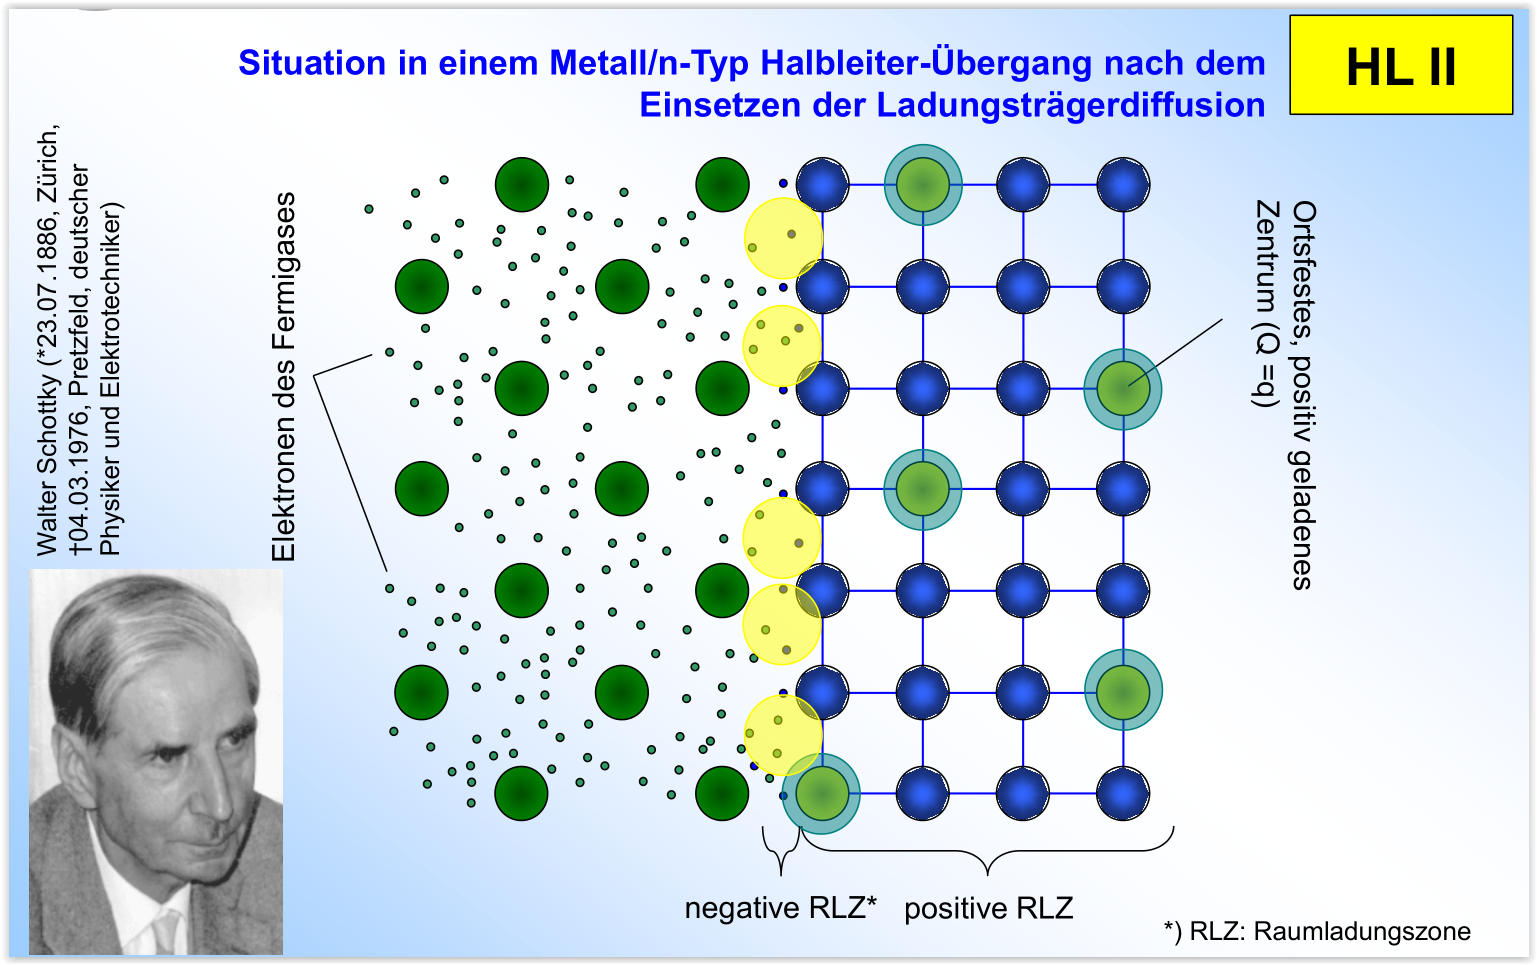
\includegraphics[width=0.95\linewidth]{schottky_m-n_nachher.png}
		  \caption{Schottky Kontakt Metall/n-Typ während der Diffusion \protect\cite{MIKRO2}}
		  \label{fig:schottky_m-n_diff}
		\end{minipage}
  \end{figure}
  \begin{figure}[H]
	  \centering
	  \captionsetup{justification=centering}
	  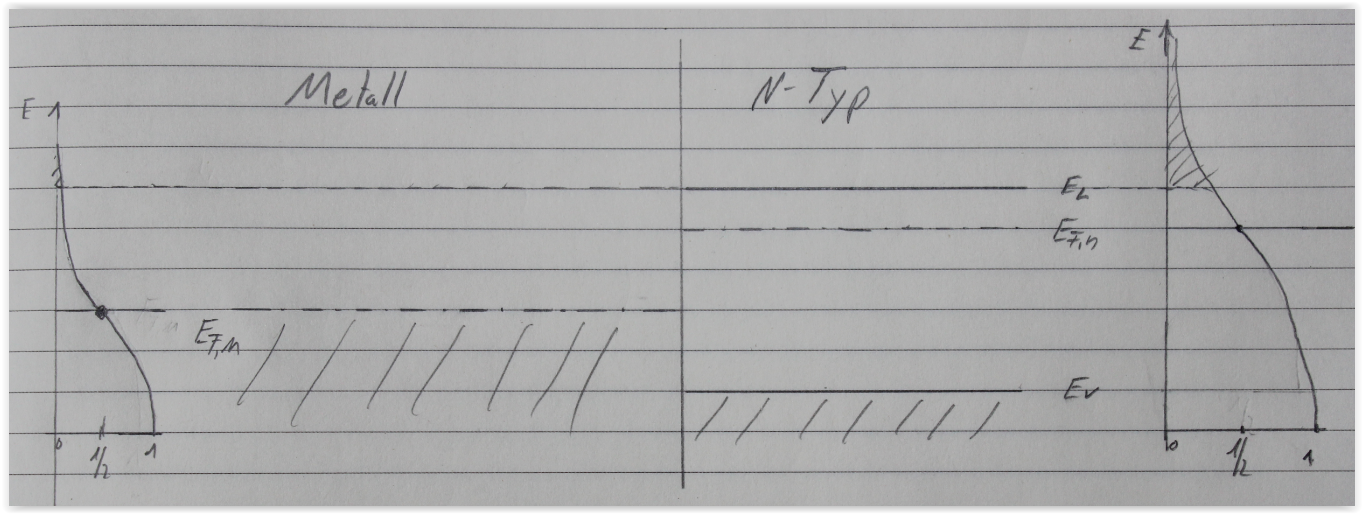
\includegraphics[width=0.8\linewidth]{schottky_m-n_banddiagramm.png}
	  \caption{Schottky Kontakt Metall/n-Typ Bänder (vor Kontakt)}
	  \label{fig:schottky_m-n_banddiagramm}
	\end{figure}
	Für die Diffusionsrichtung gilt:
	\begin{align}
	  \Phi_{MS} = \Phi_M - \Phi_S < 0 \Rightarrow \text{Metall } \rightarrow \text{ Si} \\
	  \Phi_{MS} = \Phi_M - \Phi_S > 0 \Rightarrow \text{Si } \rightarrow \text{ Metall}
	\end{align}
	Nach dem Kontakt kommt es zu einer Bandverbiegung sodass ohne Zuführung von Energie die Barriere für die Elektronen nicht überwindbar ist (siehe Abbildung \ref{fig:schottky_m-n_banddiagramm_nach}).
	\begin{figure}[H]
	  \centering
	  \captionsetup{justification=centering}
	  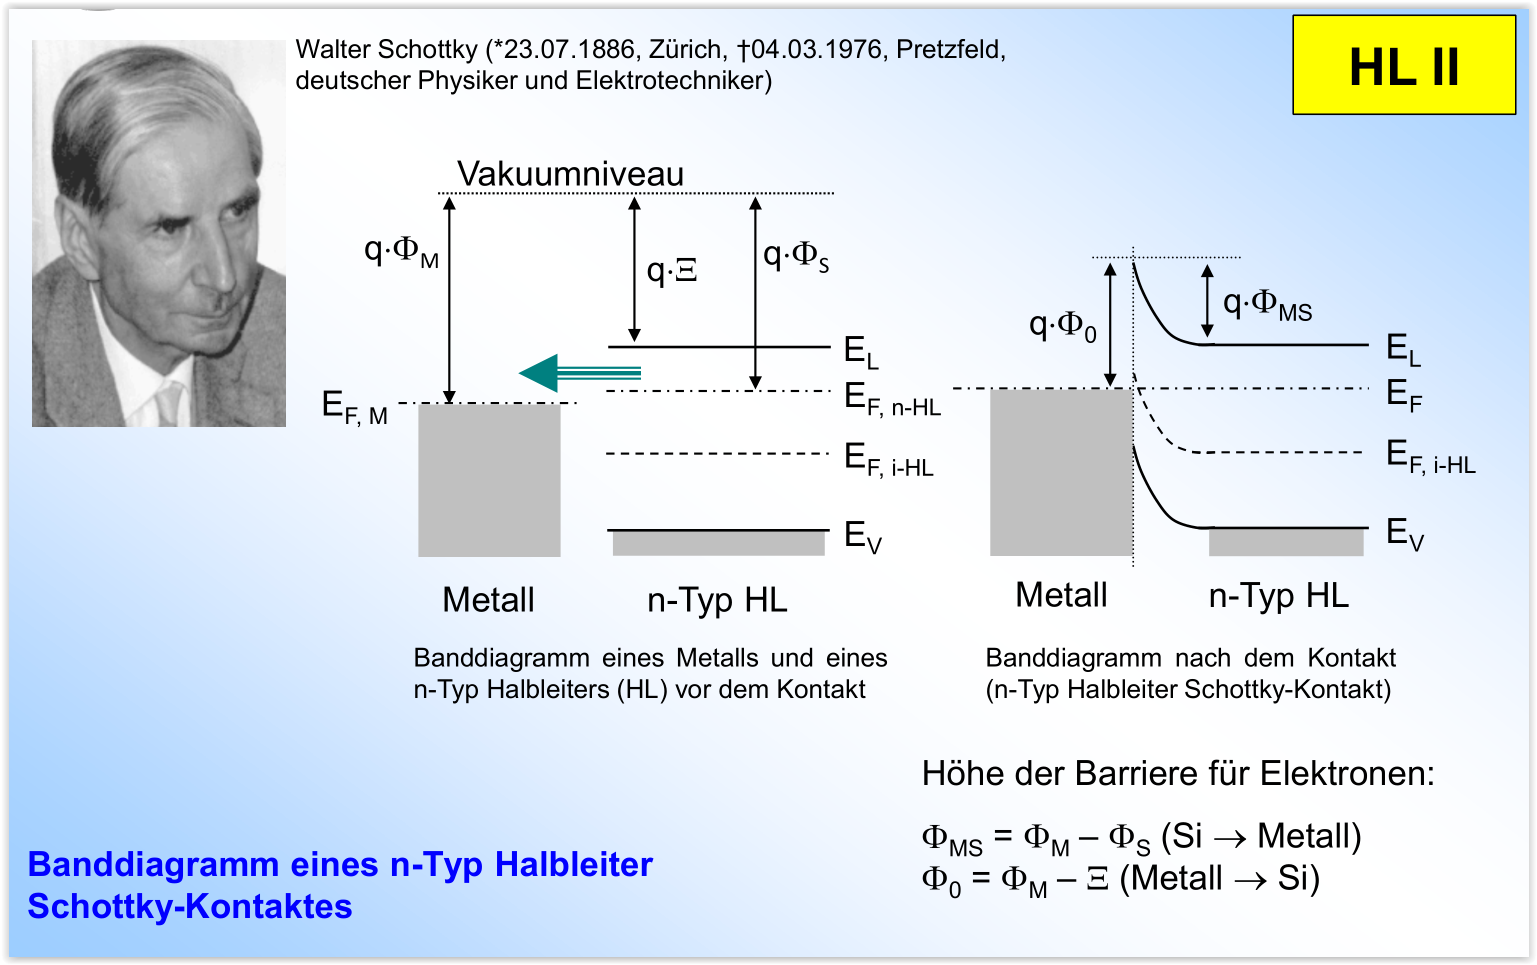
\includegraphics[width=0.6\linewidth]{schottky_banddiagramm_n.png}
	  \caption{Schottky Kontakt Metall/n-Typ Bänder (nach Kontakt) \protect\cite{MIKRO2}}
	  \label{fig:schottky_m-n_banddiagramm_nach}
	\end{figure}
	\newpage
	
  \section{07. Juli 2018: Vorlesung 10}
	  \subsection{Schottky-Kontakt}
			\subsubsubsection{Metall/p-Typ Halbleiter Übergang}
			 Wie in Abbildung \ref{fig:schottky_m-p} sichtbar ist der Halbleiter nun mit Akzeptoren dotiert die jeweils ein Siliziumatom frustrieren und somit einen Akzeptorzustand erzeugen. Das Fermi-Niveau des Metalls ist nun höher als das des Halbleiters und es diffundieren Elektronen vom Metall in den Halbleiter. Wie in \ref{fig:schottky_m-p_banddiagramm_nach} dargestellt werden zunächst durch Elektronen aus dem Metall die frustrierten Siliziumatome befriedigen. Dadurch lädt sich der Halbleiter negativ auf, das Metall wiederum positiv und so entsteht eine RLZ an der Grenzfläche. Hier ist die negative Raumladungszone ausgedehnt.
			\begin{figure}[H] 
				\centering
				\begin{minipage}{.5\textwidth}
				  \centering
				  \captionsetup{justification=centering}
				  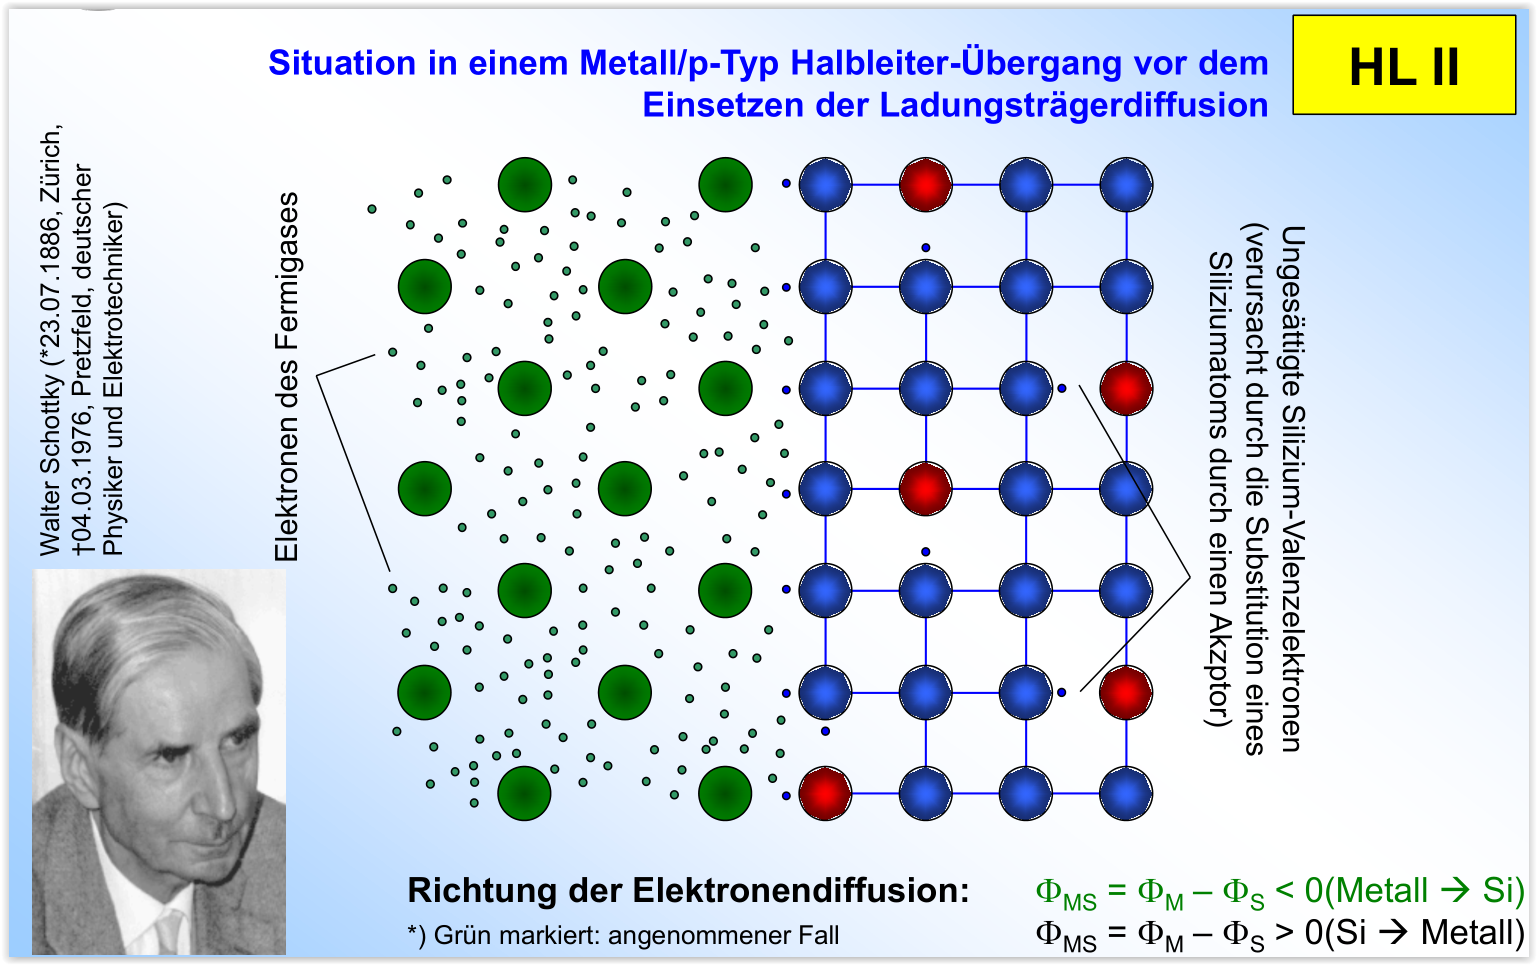
\includegraphics[width=0.95\linewidth]{schottky_m-p_vorher.png}
				  \caption{Schottky Kontakt Metall/p-Typ vor der Diffusion \protect\cite{MIKRO2}}
				  \label{fig:schottky_m-p}
				\end{minipage}%
				\begin{minipage}{.5\textwidth}
				  \centering
				  \captionsetup{justification=centering}
				  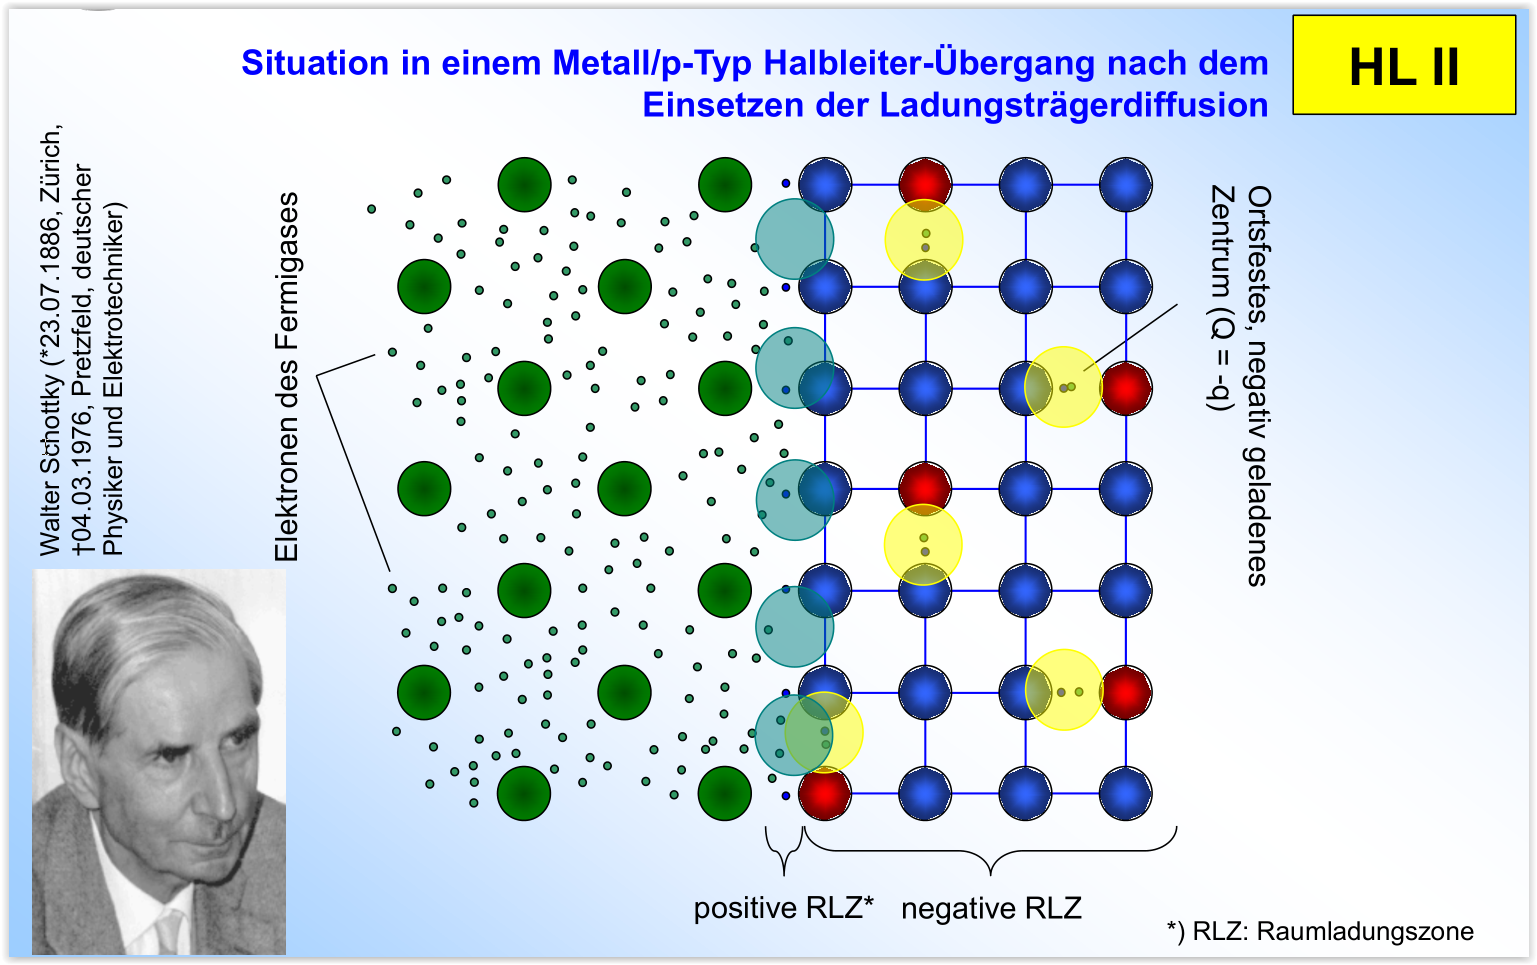
\includegraphics[width=0.95\linewidth]{schottky_m-p_nachher.png}
				  \caption{Schottky Kontakt Metall/p-Typ während der Diffusion \protect\cite{MIKRO2}}
				  \label{fig:schottky_m-p_diff}
				\end{minipage}
		  \end{figure}
			Für die Diffusionsrichtung gilt:
			\begin{align}
			  \Phi_{MS} = \Phi_M - \Phi_S < 0 \Rightarrow \text{Metall } \rightarrow \text{ Si} \\
			  \Phi_{MS} = \Phi_M - \Phi_S > 0 \Rightarrow \text{Si } \rightarrow \text{ Metall}
			\end{align}
			Das Bänderdiagramm wie in \ref{fig:schottky_m-p_banddiagramm_nach} dargestellt biegen sich die Bänder nun nach unten. Auch hier ist der Vorgang wieder unipolar, denn der Stromtransport wird im P-Typ Halbleiter primär durch Löcher im Valenzband getragen. AUch hier erkennt man wieder eine Barriere die die Elektronen bzw. Löcher zunächst überwinden müssen. Wird eine äussere Spannung angelegt wird die RLZ größer und es werden noch mehr Elektronen abgesaugt.
		  \begin{figure}[H]
			  \centering
			  \captionsetup{justification=centering}
			  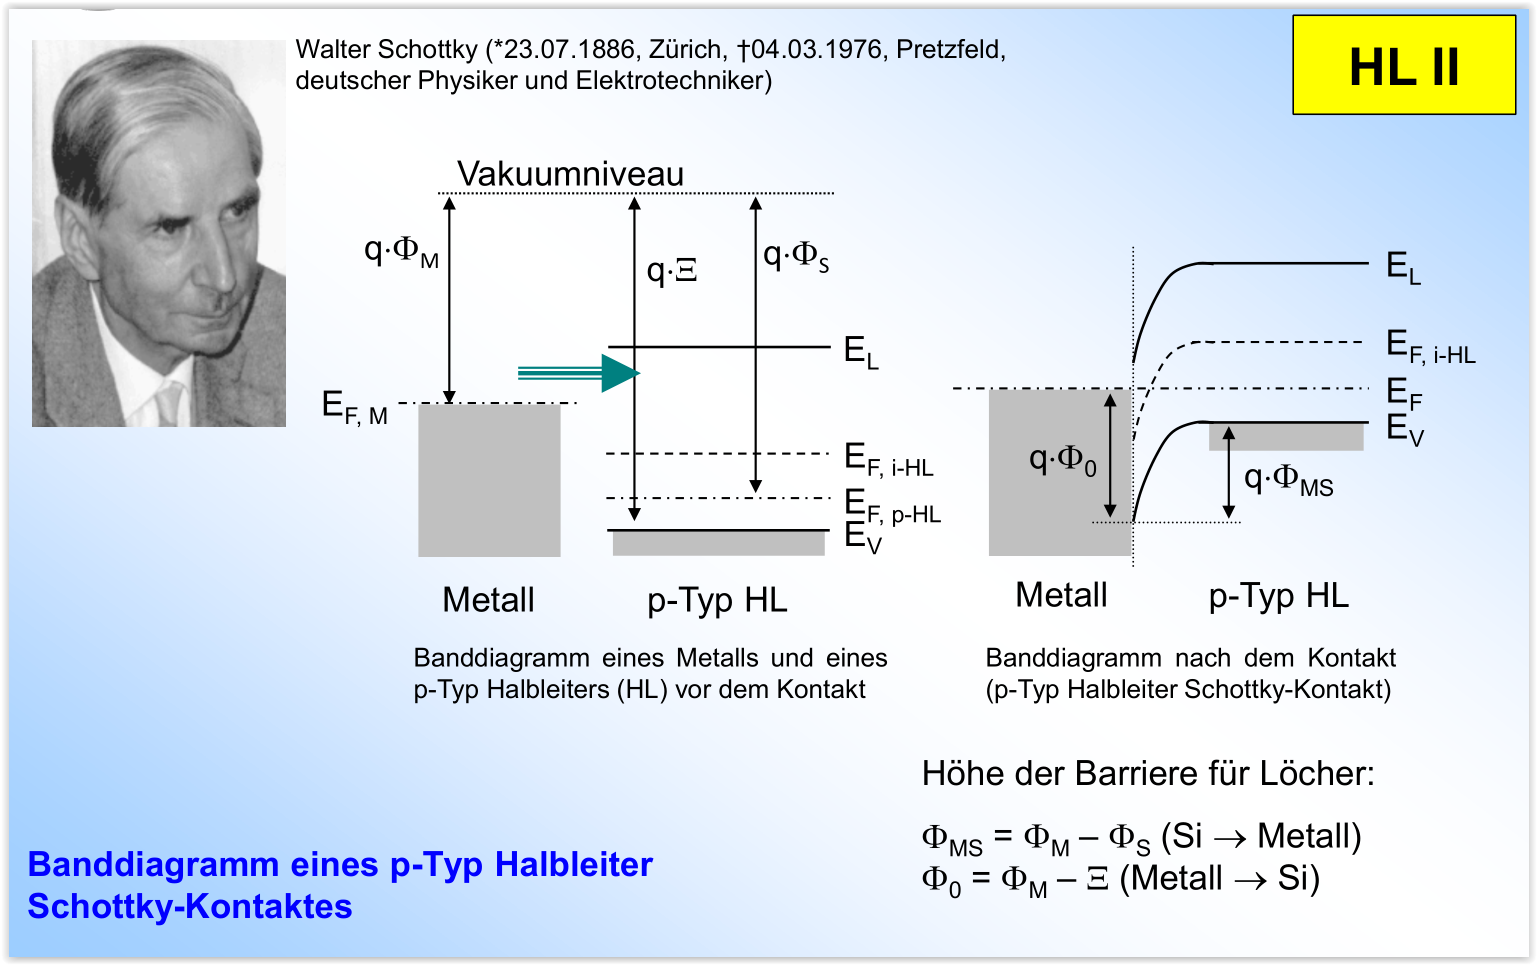
\includegraphics[width=0.6\linewidth]{schottky_banddiagramm_p.png}
			  \caption{Schottky Kontakt Metall/p-Typ Bänder (nach Kontakt) \protect\cite{MIKRO2}}
			  \label{fig:schottky_m-p_banddiagramm_nach}
			\end{figure}
			
    \subsection{MISFET}
      \begin{figure}[H]
			  \centering
			  \captionsetup{justification=centering}
			  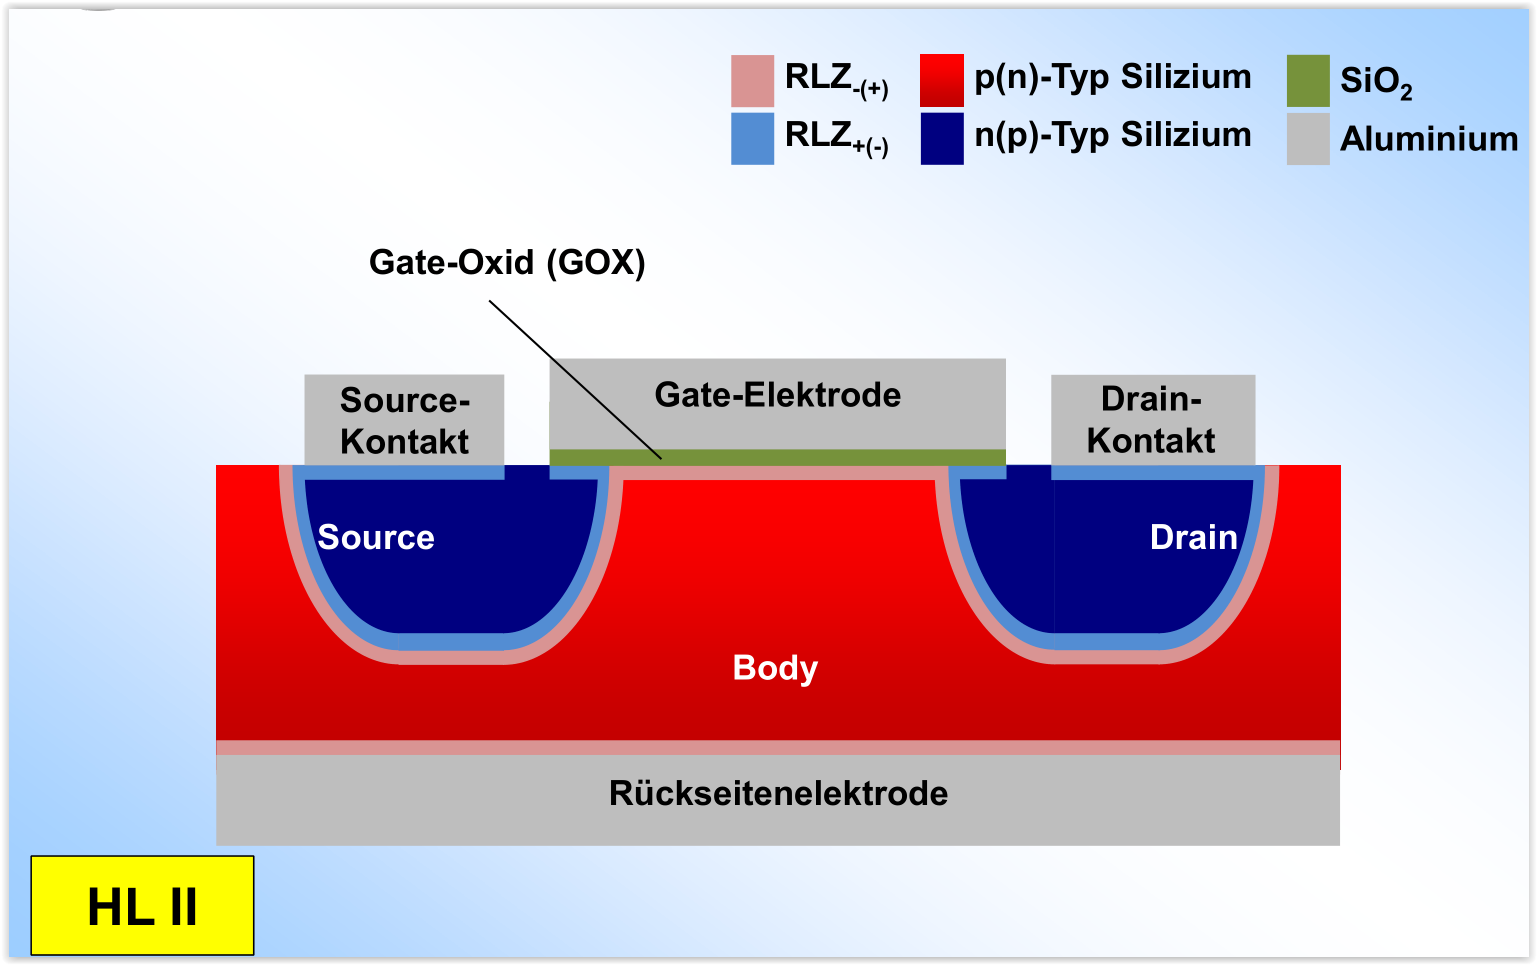
\includegraphics[width=0.6\linewidth]{misfet_aufbau.png}
			  \caption{Aufbau Misfet \protect\cite{MIKRO2}}
			  \label{fig:misfet_aufbau}
			\end{figure}
			Grundsätzlich erkennt man die Serienschaltung zweider Dioden, die gegenläufig zueinander geschalten sind (PN und NP). Damit kann eigentlich kein Stromfluss (ausser dem Sperrstrom) zustande kommen, da ein PN Übergang immer in Sperr- und einer in Durchlassrichtung ist. Legt man nun eine Gatespannung an influenziert sich ein Inversionskanal der mit Elektronen geflutet wird (siehe Abbildung \ref{fig:misfet_inversionskanal}). Der Kanal verhält sich wie ein $n+$ dotiertes Gebiet. Der Widerstand durch den Inversionskanal ist dabei um Größen kleiner als über den Body und somit fließt der Strom durch den Inversionskanal. In Abbildung \eqref{fig:misfet_stromfluss} ist das Ersatzschaltbild dargestellt. Betrachtet man nun die Schottky Kontakte erkennt man, dass auch eine dieser beiden Schottky Dioden immer in Sperrrichtung gepolt sein muss und somit wieder kein Stromfluss zustande kommen dürfte. Dieses Problem stellt sich bei allen Halbleiterbauelementen, nicht nur beim MIS- bzw. MOSFET.
			\begin{figure}[H] 
				\centering
				\begin{minipage}{.5\textwidth}
				  \centering
				  \captionsetup{justification=centering}
				  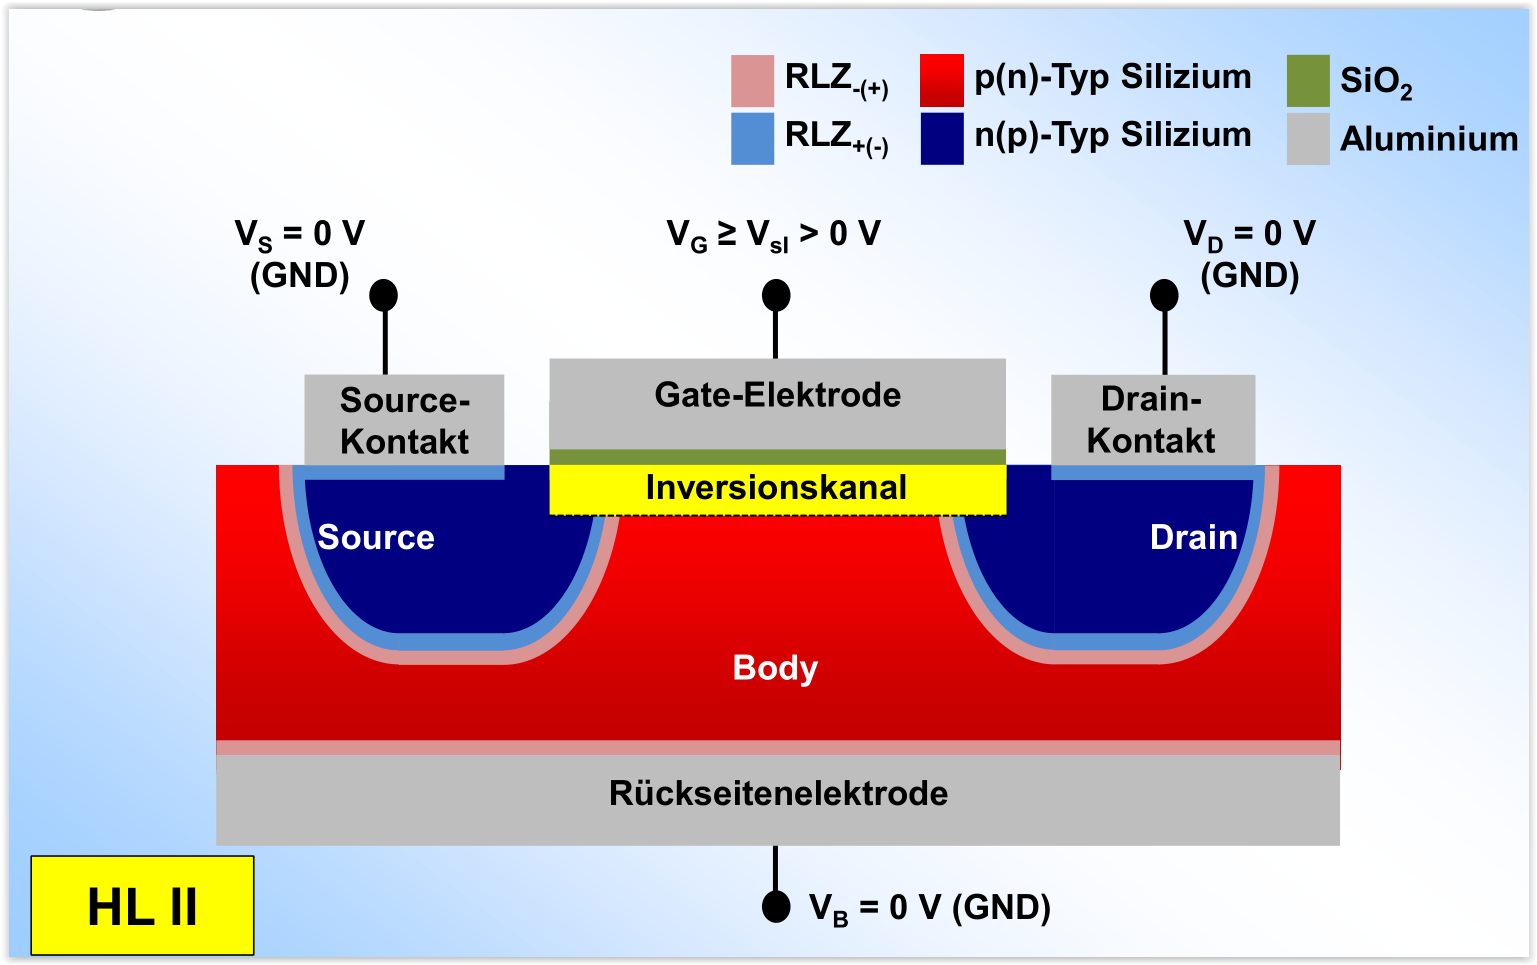
\includegraphics[width=0.95\linewidth]{misfet_inversionskanal.png}
				  \caption{MISFET Inversionskanal \protect\cite{MIKRO2}}
				  \label{fig:misfet_inversionskanal}
				\end{minipage}%
				\begin{minipage}{.5\textwidth}
				  \centering
				  \captionsetup{justification=centering}
				  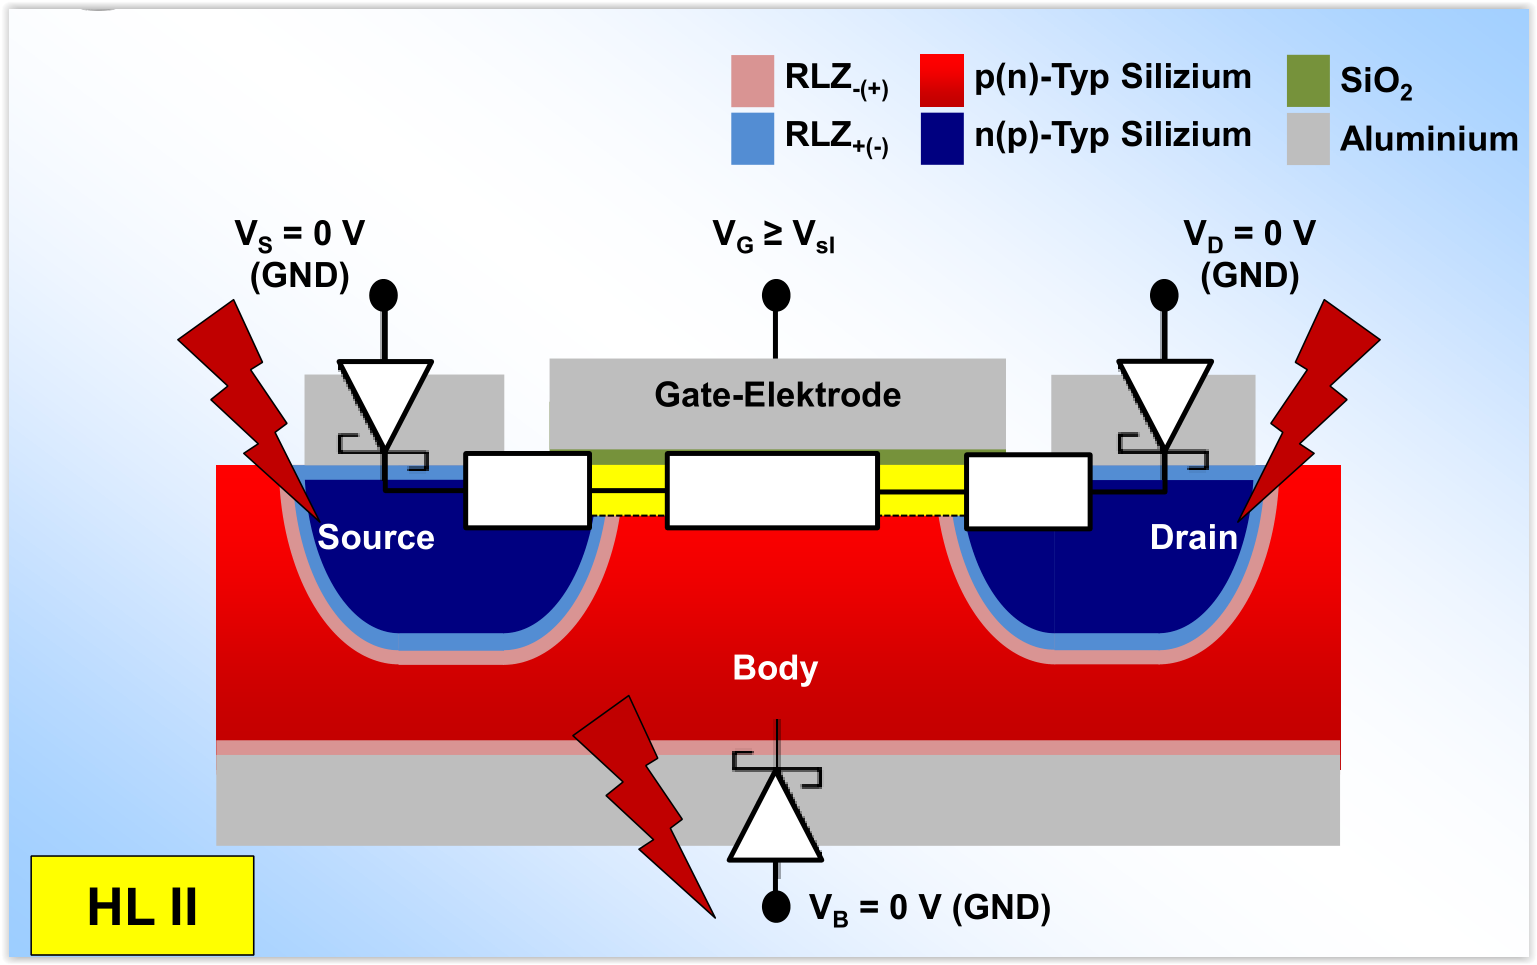
\includegraphics[width=0.95\linewidth]{misfet_stromfluss.png}
				  \caption{MISFET Ersatzschaltbild \protect\cite{MIKRO2}}
				  \label{fig:misfet_stromfluss}
				\end{minipage}
		  \end{figure}
    Um dieses Problem zu lößen, dotiert man den Halbleiter genau am Schottky Kontakt immer höher. Dotiert man den n-Typ Halbleiter immer höher, dann schiebt sich das Fermi Niveau immer näher ans Leitungsband. Die Barriere rutscht so immer näher an den PN-Übergang. Schiebt man die Barriere nah genug an den PN-Übergang ($<5nm$), also dotiert man extrem hoch ($\sim 10^{20}cm^{-3}$), verhält sich der Schottky Kontakt wie ein ohmscher Kontakt. Man spricht hier von einem ohmschen Tunneldurchgang (Quantenphysik). Die Elektronen durchtunneln die Barriere dabei einfach als wäre sie nicht vorhanden. Das Teilchen zeigt dabei Wellencharackter. Die Tunnelwahrscheinlichkeit ist gegeben durch
    \begin{equation}
      |D(G)|^2 \sin e^{-2G}
    \end{equation}
    Wobei $G$ der Gamowfaktor ist.
    \begin{equation}
      G = \int\limits_{-\frac{a}{2}}^{\frac{a}{2}} \sqrt{\frac{2\cdot m}{\hbar^2}\cdot (V_0 - E_{ges})}dx
    \end{equation}
    Der Gamowfaktor ist beeinflussbar über drei Größen. 
    \begin{itemize}
      \item Je kleiner die Barriere, also je näher die Inegrationsgrenzen beieinander sind, desto höher ist die Tunnelwahrscheinlichkeit
      \item Je kleiner die Masse, desto höher desto höher ist die Tunnelwahrscheinlichkeit
      \item Je kleiner die Gesamtenergie relativ zur Barrierenhöhe ist, desto höher ist die Tunnelwahrscheinlichkeit
    \end{itemize}
    
    \subsection{Bipolartransistor}
    \subsubsection{Aufbau}
    In Abbildung \ref{fig:bpt_aufbau} erkennt man deutlich, dass der BPT (Bipolartransistor) im Gegensatz zum MISFET ein asymmetrisches Bauelement ist. Der eigentliche Transistor der gelb eingerahmte Bereich. Alles weitere ist zur reinen Kontaktierung. Die Basis ist dabei mit $20-30nm$ sehr dünn. Die Basis muss entsprechend dünn sein damit der Transistor extrem schnell schalten kann. Die herausgeführte Basis mit dem P-Typ dotierten Teil ist nur zur Kontaktierung. Ebenfalls asymmetrisch am BPT ist ungleichmäßige Dotierung. Der Emitter zeichnet sich dadurch aus die höchstdotierteste Zone zu sein. Der Kollektor (der $n-$ markierte Bereich) ist im Gegensatz dazu sehr schwach dotiert. Z.B.:
    \begin{itemize}
      \item Emitter: $10^{20}cm^{-3}$
      \item Basis:  $10^{18}cm^{-3}$
      \item Kollektor:  $10^{15} - 10^{16}cm^{-3}$
    \end{itemize}
    Würde man an den Kollektor direkt einen Kontakt anbringen würde sich eine Schottky Diode bilden. Um die Problematik zu umgehen nutzt man eine erneut sehr hoch dotierte Schicht die wiederrum nur zur Kontaktierung da ist.
    \begin{figure}[H]
			  \centering
			  \captionsetup{justification=centering}
			  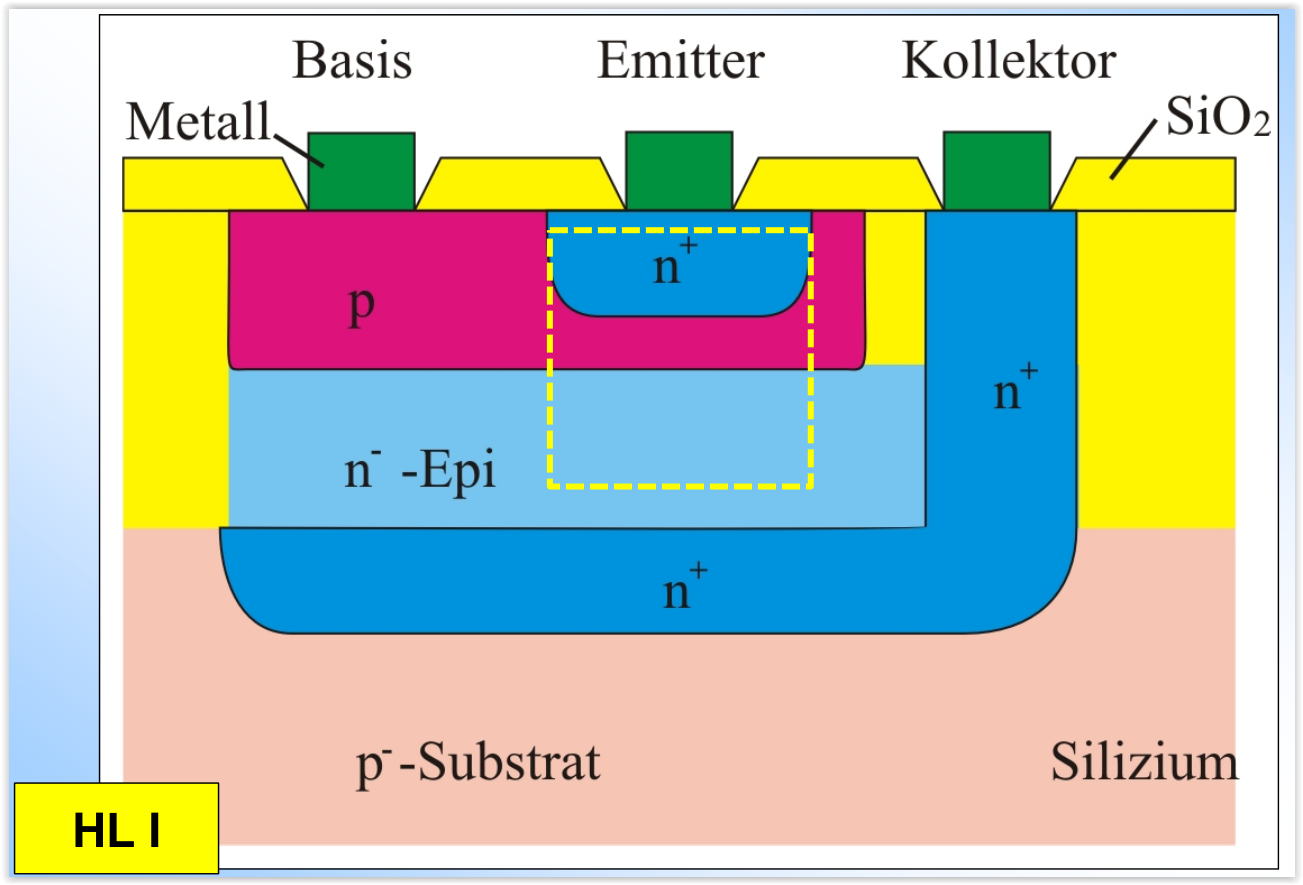
\includegraphics[width=0.6\linewidth]{bpt_aufbau.png}
			  \caption{Aufbau NPN Bipolartransistor \protect\cite{MIKRO2}}
			  \label{fig:bpt_aufbau}
		\end{figure}
		\subsubsection{Symbolik}
    \begin{figure}[H]
			  \centering
			  \captionsetup{justification=centering}
			  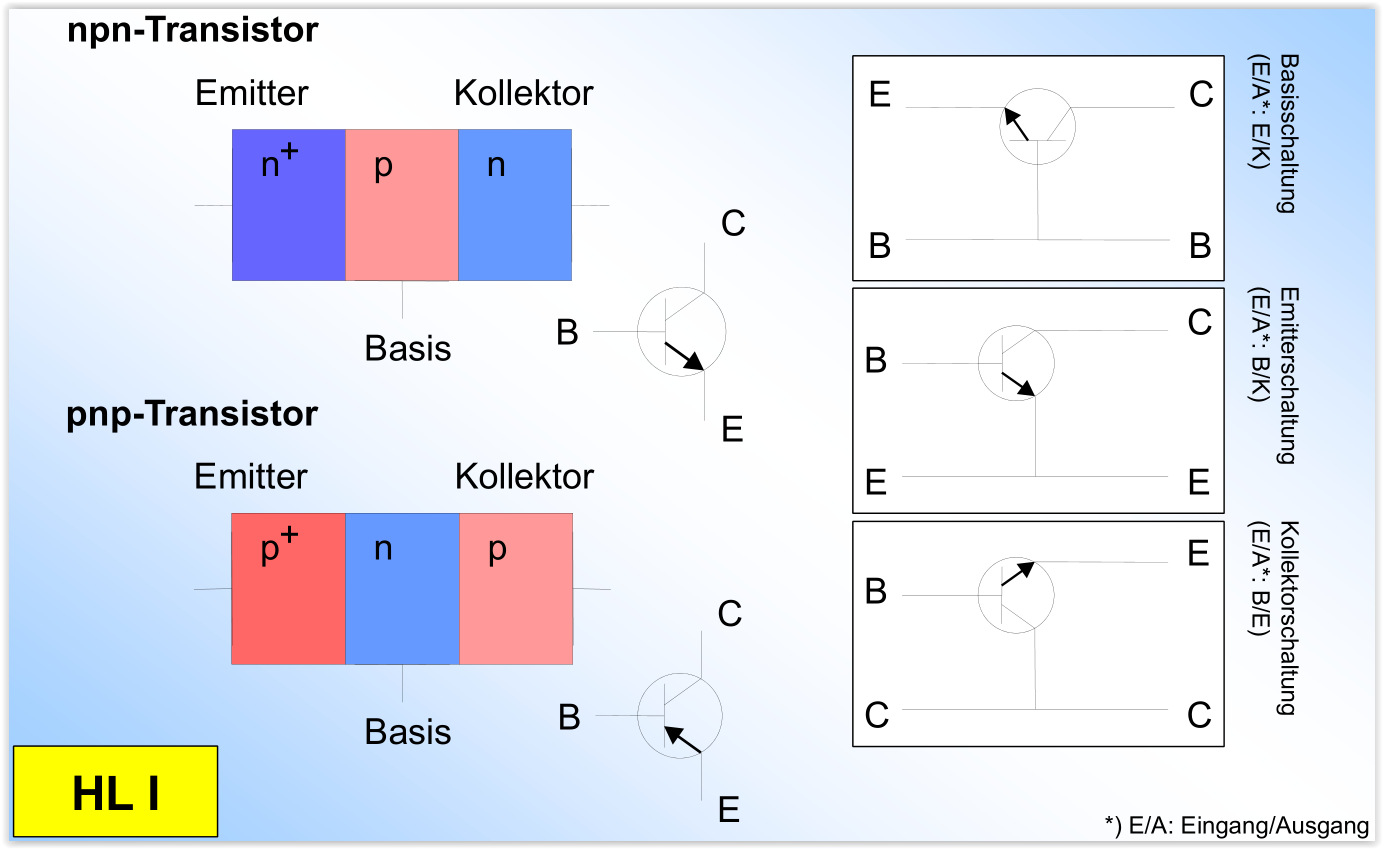
\includegraphics[width=0.6\linewidth]{bpt_symbolik.png}
			  \caption{Symbolik Bipolartransistor \protect\cite{MIKRO2}}
			  \label{fig:bpt_symbolik}
			\end{figure}
		Eselsbrücke zum Schaltzeichen: \ul{P}feil \ul{N}ach \ul{P}latte = PNP	
		\subsection{Some facts}
				\begin{itemize}
				  \item Der Schottky Kontakt ist ein unipolares Bauelement (läuft im Leitungsband ab und wird hauptsächlich von Elektronen getragen.
				  \item Schottky Dioden sind die schnellsten Dioden da $\mu_n > \mu_p$
				  \item Flachbandzustand: Elektrisches Feld bricht komplett zusammen
				  \item Ist die Frequenz hoch genug dann verhält sich eine Gleichrichterdiode wie ein Widerstand und der Strom wird nicht mehr in eine Richtung gesperrt
				  \item Auf dem Weg vom P ins N Gebiet einer PN Diode werden Löcher zu 100\% in Elektronen umgewandelt. Dadurch ist der PN-Übergang langsamer als der Schottky Kontakt
				  \item Si-Diode Ventilspannung: $\sim 0,7V$; Schottky-Diode: $\sim 0,3V$ (da RLZ nur halbseitig)
				  \item Je höher die Dotierung, umso kleiner wird die RLZ
				    \begin{itemize}
				      \item $10^{15} - 10^{16}cm^{-3}$ $\rightarrow$ RLZ $\sim 10^{-6}m$
				      \item $10^{18}cm^{-3}$ $\rightarrow$ RLZ $\sim$ mehrere $100\cdot 10^{-9}m$
				      \item $10^{20}cm^{-3}$ $\rightarrow$ RLZ $\sim$ wenige  $10^{-9}m$
				    \end{itemize}
				    \item Der Begriff evaleszente Welle beschreibt die Totalreflexion bei Licht- und Wasserwellen mit unterschiedlich großen Spalten
				    \item Der Bipolartransistor ist das schnellste schaltbare Bauelement
				\end{itemize}
	\newpage
	
  \section{10. Juli 2018a: Vorlesung 11a}
  \subsection{Erdpotential}
  \begin{itemize}
    \item Die Erde stellt Elektronen zur Verfügung bzw. nimmt sie auf
    \item Erde zeigt passives Verhalten, das heißt sie nimmt nur Elektronen auf bzw. gibt nur Elektronen ab wenn sich dazu angeregt wird
    \item Erste Experimente wurden durch Benjamin Franklin durchgeführt
  \end{itemize}
  \begin{definition}
    \begin{equation}
      v = \frac{I_{out}}{I_{in}}
    \end{equation}
  \end{definition}
    \subsection{Funktionsweise eines NPN-BPT}
    Der Emitter ist mit $10^{20}cm^{-3}$ am stärksten dotiert. Die Basis mit $10^{18}cm^{-3}-10^{19}cm^{-3}$ etwas weniger stark und der Kollektor mit $10^{15}cm^{-3}$ am schwächsten. Der Emitter-Basis Kreis ist nun in Vorwärtsrichtung gepolt. Es existiert noch ein RLZ aber sie ist entsprechend stark verkleinert. Am hochdotierten Emitter ist die RLZ entsprechend kleiner als an der schwächer dotierten Basis. Beide PN-Übergänge sind asymmetrisch. Der Basis-Kollektor PN-Übergang ist in Sperrichtung gepolt, daher muss die RLZ deutlich größer ausfallen.
    \subsubsection{Emitterschaltung}
     Betrachtet man die Emitterverschaltung ist die Basis der aktive Eingang.
    \begin{itemize}
      \item[1.) ] Anlegen von Spannung an die Basis: \newline
        Zunächst werden durch das Anlegen einer positiven Spannung Elektronen aus der Basis abgesaugt. Bei einem Halbleiter ist das gleichbedeutend mit einem Löcherstrom. Die Konzentration an Löchern in der Basis ist bei Raumtemperatur durch die Dotierung gegeben. Es gilt $p \approx N_A$. Von unten werden weitere Löcher injiziert, also ist die Lochkonzentration unten höher als im Rest der Basis. Damit ist ein Konzentrationsgradient vorhanden und die Löcher diffundieren weiter in die Basis hinein. 
        \item[2.) ] Diffundieren der Löcher in die Basis: \newline
        Die Löcher können prinzipiell in alle drei Raumrichtungen diffundieren. Wir betrachten die Fälle a) in die Basis hinein, b) zum Emitter und c) zum Kollektor. 
        \begin{itemize}
          \item[a) ] Die Löcher diffundieren bis der Gradient ausgeglichen ist. 
          \item[b) ] In der Basis-Emitter (BE) RLZ existiert ein inneres el. Feld, dass von der Emitter RLZ zur Basis RLZ gerichtet ist. Damit werden die Löcher die von der Basis her in Richtung BE-RLZ diffundieren direkt wieder abgestossen.
          \item[c) ] In der Basis-Kollektor (BC) RLZ ist das el. Feld vom Kollektor zur Basis gerichtet. Demzufolge werden die Löcher wie bei Fall b) auch wieder abgestossen.
        \end{itemize}
        Damit ergibt sich das Verhalten, dass der überwiegende Teil der Löcher in der Basis verbleibt. \newline
        Es muss jedoch beachtet werden, dass die in die Basis injizierte Löcher unterschiedliche Energie haben. Da es sich hierbei um Bewegung von Löchern handelt betrachtet wir in erster Linie die kinetische Energie. Hierzu betrachtet man die Maxwell-Boltzmann Verteilung, die das Quadrat des Betrags der Geschwindigkeit mit der Anzahl ins Verhältnis setzt. Der überwiegende Teil der Elektronen (schraffiert  in Abbildung \ref{fig:maxw_boltz_vert}) ist nicht schnell genug um gegen das el. Feld anzukämpfen. Dennoch gibt es doch einige Löcher die schnell genug sind (alles rechts von der gestrichelten Linie in Abbildung \ref{fig:maxw_boltz_vert}), um einen der PN-Übergänge zu überwinden. Es ist zu beachten, dass es sich aufgrund der Polung um asymmetrische PN-Übergänge handelt. Die Energie die nötig ist um den in Vorwärtsrichtung gepolten PN-Übergang zu überwinden ist deutlich geringer, da dort auch ein kleineres inneres el. Feld vorherrscht.
        \begin{figure}[H]
			  \centering
			  \captionsetup{justification=centering}
			  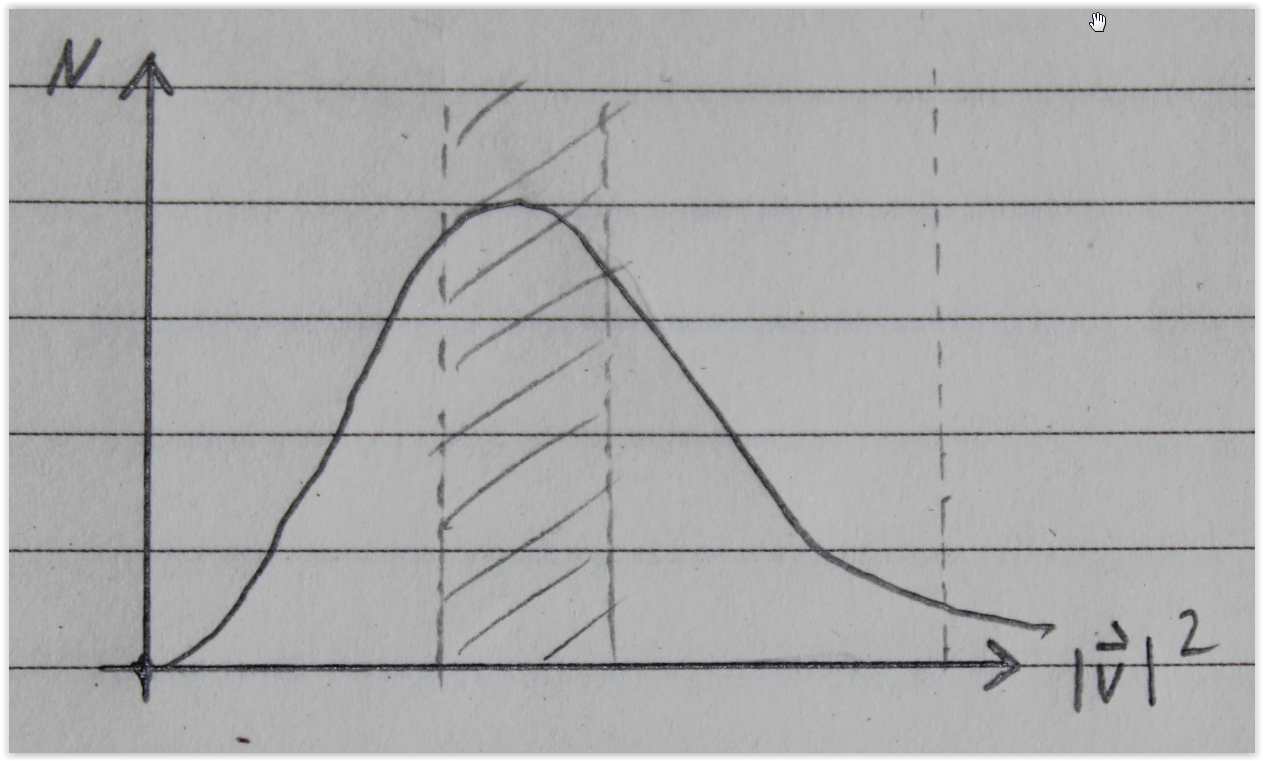
\includegraphics[width=0.4\linewidth]{maxwell_boltzmann.png}
			  \caption{Maxwell-Boltzmann Verteilung}
			  \label{fig:maxw_boltz_vert}
			\end{figure}
			Damit wird klar, der überwiegende Teil der Löcher bleibt in der Basis, ein kleiner Teil an Löchern, der schnell genug ist schafft es durch den Emitter-Basis PN-Übergang und ein sehr sehr kleiner Teil ist schnell genug und fliegt statistisch gesehen auch in die richtige Richtung um den Kollektor-Basis PN-Übergang zu überwinden. Dieser Teil ist allerdings vernachlässigbar klein. \newline
			Betrachtet man ein Loch, das schnell genug ist um den Emitter-Basis PN-Übergang zu passieren, stellt man fest, dass es am Anfang eine hohe Geschwindigkeit hat, diese aber beim passieren des PN-Übergangs immer geringer wird, bis es mit einer kleineren Restgeschwindigkeit dann die RLZ verlässt und in den Emitter eindringt. 
			\item[3.) ] Über
			\begin{equation}
			  N_D >> N_A \land N_D >> n_i \Rightarrow p = \frac{n_i^2}{N_D}
			\end{equation}
			lässt sich die Lochkonzentration bestimmen. Bei Si ist $n_i = \sim 10^{10}cm^{-3}$, also ist $p = 1 cm^{-3}$, d.h. pro Kubikcentimeter finden wir ein Loch. Auf den Emitter kommt nun eine Lawine an Löchern zu. D.h. es entsteht ein gigantischer Lochkonzentrationsgradient. Also diffundieren die Löcher in den Emitter. Dabei wird ein Teil der Löcher auf dem Weg durch den Emitter (abhängig von der Diffusionslänge) rekombinieren und ein kleiner Teil den Metallanschluss erreichen und somit über Erde abfließen. Insbesondere in dem Bereich nahe an der RLZ ist die Rekombination von Löchern mit Elektronen besonders stark. Durch die Rekombination an der Grenze zum PN-Übergang nimmt die Elektronenkonzentration in diesem Bereich stark ab. Dabei entsteht ein Elektronenkonzentrationsgradient und es kommt zu einem Diffusionsstrom von Elektronen. Dabei wird Erde wieder aktiv und liefert gerade so viel Elektronen nach wie wegdiffundieren. Damit entsteht parallel zum Löcherstrom ein Elektronendiffusionsstrom von links nach rechts. \newline
			\item [4.) ] Einige dieser Elektronen kommen bis zum PN-Übergang. Der Großteil der Elektronen wird durch das Feld wieder abgestossen, nach der Maxwell-Boltzmann Verteilung sind jedoch einige wenige schnell genug um den PN-Übergang zu durchqueren und kommen in die Basis. In der Basis angekommen rekombiniert ein Teil an Elektronen mit den Löchern in der Basis und fließt letzten Endes über die Basis nach unten ab. Ein weiterer Teil der Elektronen erreicht den PN-Übergang zum Kollektor. Das innere el. Feld dieses PN-Übergangs beschleunigt dann das Elektron und schießt es in den Kollektor. Verschwindet wenig Elektronen werden im Kollektor rekombinieren (hauptsächlich mit dem injizierten Lochstrom), der Großteil der Elektronen fließt aber durch den Kollektor und erreicht den Anschluss. Die Emitterschaltung wird in der Regel als Verstärkerschaltung genutzt.
			\begin{figure}[H]
			  \centering
			  \captionsetup{justification=centering}
			  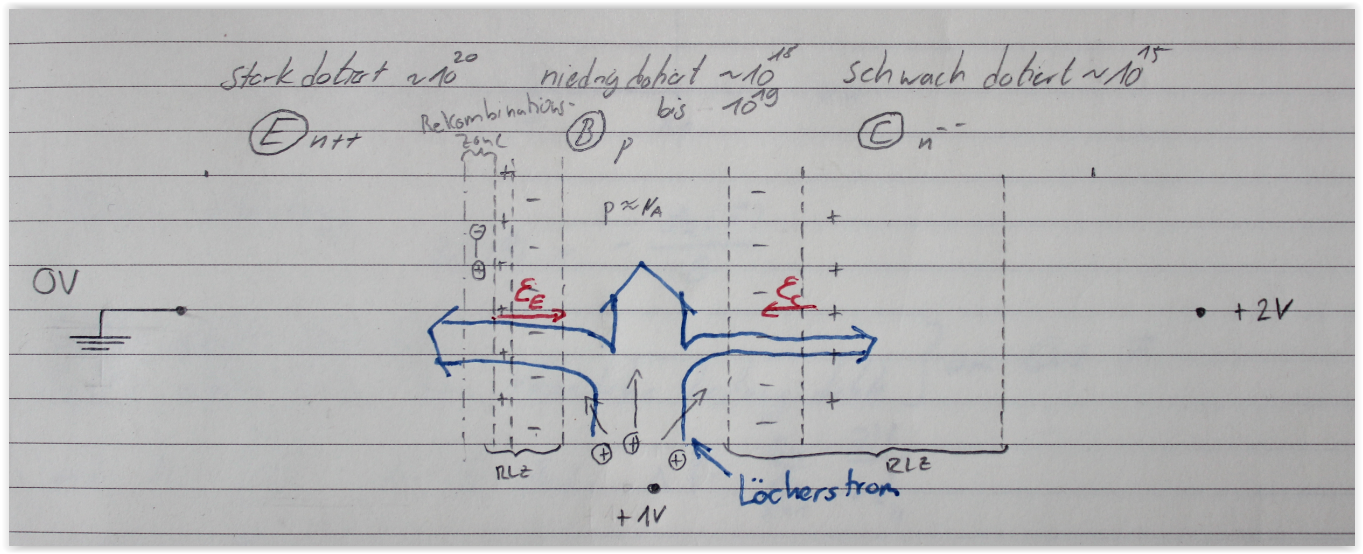
\includegraphics[width=1\linewidth]{bpt_emittersch.png}
			  \caption{Emitterschaltung Löcherstrom}
			  \label{fig:bpt_emittersch_lochstrom}
			\end{figure}
    \end{itemize}
  Im eingeschwungenen Zustand erhält man immer Abbildung \ref{fig:bpt_emittersch_lochstrom}. 
    \subsubsection{Basisschaltung}
  Wir betrachten nun die Basisschaltung. Der passive Knoten (also die Erde) ist nun an der Basis angeschlossen. Damit der Emitter-Basis PN-Übergang wieder in Vorwärtsrichtung betrieben ist muss eine negative Spannung angelegt werden. Um den Basis-Kollektor PN-Übergang wieder in Sperrrichtung zu betreiben muss eine positive Spannung am Kollektor angelegt werden.
    \begin{figure}[H]
			  \centering
			  \captionsetup{justification=centering}
			  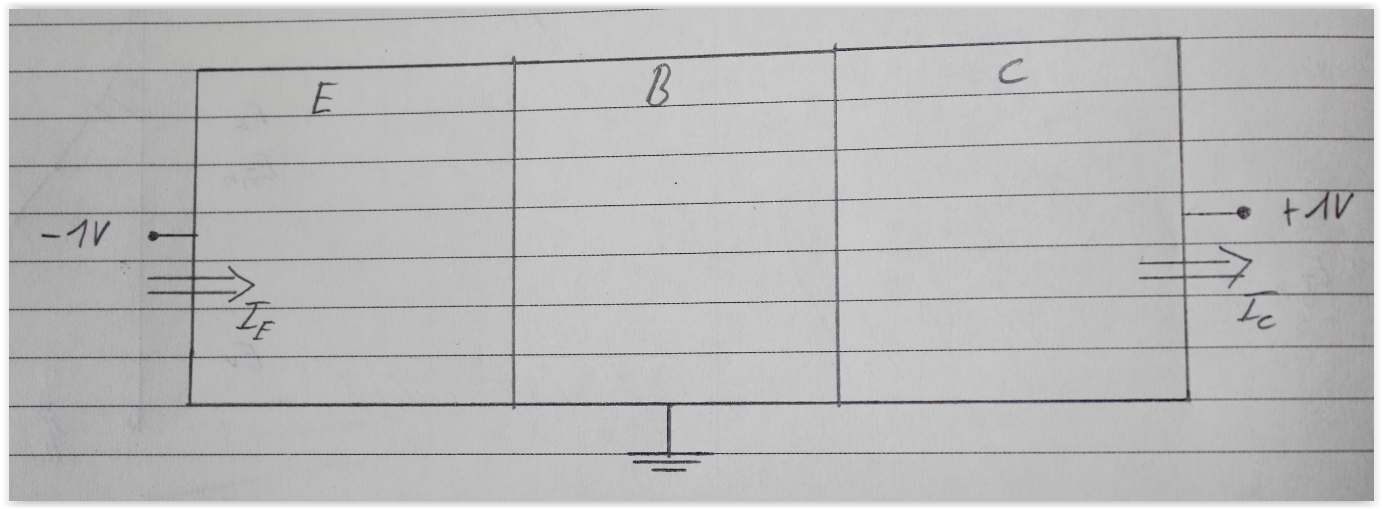
\includegraphics[width=0.6\linewidth]{bpt_basissch.png}
			  \caption{Basisschaltung}
			  \label{fig:bpt_basissch}
			\end{figure}
    \begin{itemize}
      \item[1.) ] In den Emitter werden Elektronen injiziert, die Elektronen diffundieren durch den Emitter (durch den so entstandenen Konzentrationsgradient). Es kommt da der Emitter n-Typ dotiert ist kaum zu Rekombinationen. 
      \item[2.) ] Die meisten Elektronen werden vom inneren el. Feld des Emitter-Basis PN-Übergangs abgestossen, ein Teil hat aber genug kinetische Energie um den PN-Übergang zu durchqueren und in die Basis zu gelangen.
      \item[3.) ] Es entsteht ein Elektronendiffusionsstrom. Ein Teil geht in den Kollektor und ein Teil geht in Richtung des Erdanschlusses.
        \begin{itemize}
          \item Ein Teil der Elektronen rekombiniert auf dem Weg zum Kollektor mit Löchern. Somit entsteht ein Löcherkonzentrationsgradient was die Erde dazu anregt Löcher in die Basis zu liefern. Die Elektronen die das Kollektorfeld erreichen werden davon beschleunigt und fließen über den Kollektor ab.
          \item Ein Teil der Elektronen fließt über die Basis ab.
        \end{itemize}
    \end{itemize}
    In der Basisschaltung ist die Stromverstärkung $\leq 1$, da über den Emitter Elektronen injiziert werden, allerdings fließen sowohl durch Basis als auch Kollektor Elektronen ab. Somit Ist der Ausgangsstrom durch den Kollektor auf jeden Fall kleiner als der Eingangsstrom am Emitter. Die Rekombination in der Basis ist aber oft so klein, dass von einem Faktor von $1$ ausgegangen werden kann und näherungsweise $I_E = I_C$ gilt.
    In einer Verschaltung wie in abb blabla kann eine Basis-Schaltung zur Spannungsverstärkung genutzt werden.
    \begin{figure}[H]
		  \centering
		  \captionsetup{justification=centering}
		  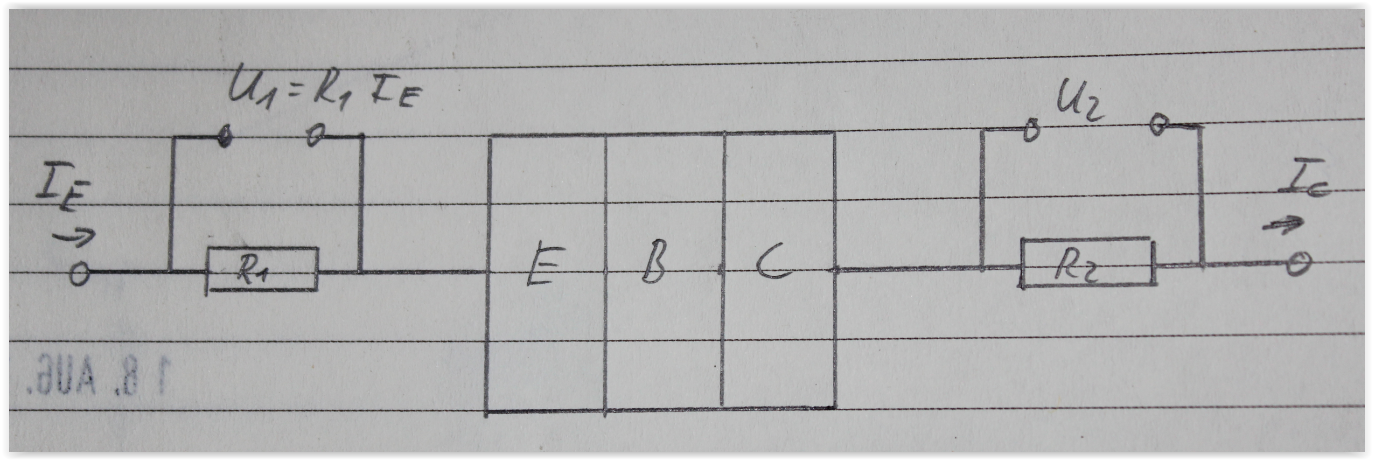
\includegraphics[width=0.6\linewidth]{bpt_basissch_spannungsverst.png}
		  \caption{Basisschaltung Spannungsverstärker}
		  \label{fig:bpt_basissch_spannungsverst}
		\end{figure}
    Ingenieursmäßig betrachtet wird das Bauelement an dem Moment interessant, an dem der in die Basis injizierte Strom anders ist als der Emitter-Kollektorstrom, bzw. beeinflusst werden kann. \newline
    
  \subsubsection{Stromverstärker}  
  Um einen guten Stromverstärker zu designen muss gewährleistet sein, dass pro injiziertes Loch mehrere Elektronen vom Emitter zum Kollektor fließen. Betrachtet man die Vorgänge ohne den Teil an Elektronen, der es durch die Basis schafft und am Kollektor abgesaugt wird, verhält es sich wie beim Einschalten einer PN-Diode. Damit gilt:
  \begin{equation}
    I_{EB} = I_S \left( e^{\frac{q U_{eb}}{K_B T}} -1\right)
  \end{equation}
  Wobei $I_S$ der Sperrsättigungsstrom ist und es gilt:
  \begin{equation}
    I_S = Aq \left(\underbrace{\frac{D_n n_{p_0}}{L_n}}_{I_n} + \underbrace{\frac{D_p p_{n_0}}{L_p}}_{I_p} \right)
  \end{equation}
  Wobei $A$ die Querschnittsfläche des Transistors ist. Bildet man nun das Injektionsverhältnis, also das Verhältnis vom Elektronenstrom zum Löcherstrom, dann erhält man:
  \begin{equation}
    \frac{I_n}{I_p} = \frac{D_n L_p n_{p_0}}{D_p L_n p_{n_0}}
  \end{equation}
  Mit $D_n \approx D_p$ und $L_n \approx L_p$ erhält man
  \begin{equation}
    \frac{I_n}{I_p} \approx \frac{N_{p_0}}{p_{n_0}} = \frac{\cancel{n_i^2}}{N_A}\frac{N_D}{\cancel{n_i^2}}
  \end{equation}
  Hierbei wird klar, bei einem symmetrischen PN-Übergang, also bei gleich großer Dotierung ist der Lochstrom gleich groß wie der Elektronenstrom. Bei einem asymmetrischen PN-Übergang verschiebt sich aber dieses Verhältnis. Das Ziel bei der Emitterschaltung ist es, mit einem kleinen Lochstrom einen hohen Elektronenstrom zu treiben. Um nun einen guten Verstärker zu bauen muss der Emitter ($N_D$) sehr stark und die Basis ($N_A$) möglichst schwach dotiert werden. Die Basis lässt sich allerdings nur zwei bis drei Größenordnungen schwächer als den Emitter dotieren, da die RLZ in Richtung Basis immer größer wird je geringer die Basis dotiert ist. Dotiert man zu stark würden sich beide RLZ irgendwann berühren und der Punch-Fall würde eintreten. In diesem Fall würde beim Anlegen einer Sperrspannung am Kollektor der BPT über den Kollektor eingeschaltet werden.
  \subsection{Some facts}
  \begin{itemize}
    \item Der Name der Transistorschaltung (Emitterschaltung, etc.) gibt an welcher Anschluss des Transistors auf Masse ist
    \item Zur Beschreibung eines Halbleiterstromes benötigt man grundsätzlich vier Terme
      \begin{itemize}
        \item Lochstrom (getrieben durch Diffusion oder el. Feld oder beides)
        \item Elektronenstrom (getrieben durch Diffusion oder el. Feld oder beides)
      \end{itemize}
  \end{itemize}
\newpage	

  \section{10. Juli 2018b: Vorlesung 11b}
  \subsection{Emitterwirksamkeit}
  \begin{definition}$\;$\newline
    $\alpha_E$ = Emitterwirksamkeit (Wahrscheinlichkeit mit der ein Elektron in die Basis kommt \newline
    $\alpha_T$ = Transportfaktor (Wahrscheinlichkeit dass ein Elektron nicht rekombiniert)
  \end{definition}
  Es gilt: 
  \begin{equation}
    I_C = \alpha_0 \cdot |I_E| = \alpha_E \cdot \alpha_T \cdot |I_E|
  \end{equation}
  \begin{definition}
    \begin{equation}
      \alpha_E := \frac{I_n}{I_n + I_p} = \frac{1}{1+\frac{I_p}{I_n}} = \frac{1}{1+\frac{D_p L_n P_{n_0}}{D_n L_p n_{p_p0}}} = \frac{1}{1+\frac{D_p L_n}{D_n L_p}\frac{N_A}{N_D}}
    \end{equation}
  \end{definition}
    Fließen extrem viele Löcher aus der Basis in den Emitter, steigt die Wahrscheinlichkeit dass ein Elektron mit einem Loch rekombiniert bevor es in die Basis gelangt. Wird also $I_p$ im Verglech zu $I_n$ immer größer dann geht $\alpha_E$ gegen Null,d.h. so gut wie keine Elektronen schaffen es in die Basis.\newline
   Wird die Basis zu breit, dann rekombiniert praktisch jedes Elektron. Der komplette Strom würde über die Basis abfließen.\newline 
   $\Rightarrow$ die Basisweite muss deutlich kleiner als die Diffusionslänge der Majoritäten sein.
   \begin{equation}
     w_B \overset{!}{<<} L_n
   \end{equation}
   Damit kann die Emitterwirksamkeit angepasst ($L_n$ durch die Basisweite ersetzen) werden:
   \begin{equation}
     \Rightarrow \alpha_E = \frac{1}{1 + \frac{D_p}{D_n} \displaystyle\frac{w_b N_A}{L_p N_D}}
   \end{equation}
   Wobei $N_A$ die Dotierkonzentration in der Basis ist und möglichst niedrig sein sollte und $N_D$ die Dotierkonzentration im Emitter ist und möglichst hoch sein sollte. \newline
   
   \subsection{Transportfaktor}
   Nähert man sich dem Konzentrationsgradient mit dem Dreieck $\frac{n-0}{w}$ an erhält man für $|I_E|$:
   \begin{equation}
     |I_E| = A_q D_n \frac{n(0)-0}{w_B}
   \end{equation}
   Schätzt man nun Rekombinationswahrscheinlichkeit $\sim$ Anzahl der Elektronen $\sim$ Anzahl der Löcher ab und setzt man $A_{Dreieck} \sim$ Anzahl der Elektronen in der Basis so erhält man
   \begin{equation}
     |I_B| = Aq \frac{n(0)w_B}{2}\frac{1}{\tau_n}
   \end{equation}
   \begin{equation}
     \alpha_T = \frac{|I_C|}{|I_E|} = 1 - \frac{1}{2}\left(\frac{w_B}{L_n}\right)^2
   \end{equation}
   
   \subsection{Stromverstärkung in Emitterschaltung}
   \begin{equation}
     \beta_0 = \frac{I_C}{I_B} = \frac{\alpha_0}{1-\alpha_0}
   \end{equation}
   \subsection{Feldeffekt}
   \begin{definition}
     Feldeffekt bedeutet, dass bei einem leitfähigen Material, durch ein elektrisches Querfeld das senkrecht dazu angreift, die Leitfähigkeit der oberflächennahen Schicht verändert wird. Dieser Effekt kann nur bei Halbleitern auftreten.
   \end{definition}
     \subsubsection{Elektrische Felder und Materialklassen}
     \begin{table}[H]
       \centering
       \begin{tabular}{P{3cm} | p{9cm}}
         Isolator & Elektrisches Feld geht unabhängig von der Stärke zu 100\% durch \\
         Metall & Stoppt das elektrische Feld komplett \\
         $\;$\newline Halbleiter & Stoppt das elektrische Feld teilweise, es dringt aber bis zu einer gewissen Tiefe ein (bis die Feldlinien auf einen Ladungsträger treffen der sie terminiert)
       \end{tabular}
     \end{table}
     \subsubsection{Feldeffekt beim MISFET} \label{subsubs:misfet_feldeffekt}
     Wie in Abbildung \ref{fig:misfet_feldeffekt_a} dargestellt bildet sich beim Anlegen einer positiven Spannung an di Gate-Elektrode ein elektrisches Feld von den als rotes Plus markierten positiven Ladungsträgern in Richtung des Bodies des FETs. Durch den $SiO_2$ Isolator gehen die Feldlinien ungehindert hindurch. Die Feldlinien dringen so tief in den Halbleiter ein, bis sie durch eine negative Ladung terminiert werden. Im p-dotierten Body gibt es mit $\frac{n_i^2}{N_A}$ nur sehr wenig Elektronen, sodass das elektrische Feld relativ tief in dein Halbleiter eindringen wird. Im Halbleiter laufen weiterhin immer Rekombinations- und Generationsprozesse ab. Das elektrische Feld separiert damit sofort die generierten Elektronenlochpaare und saugt entsprechend der Polarität die Elektronen zur Grenzfläche und schiebt die Löcher nach unten. Damit ist die Rekombination dort wo das Feld wird stark behindert. Die Löcher die nach unten geschoben werden diffundieren nach unten über die Rückseitenelektrode auf die Erde ab. An der Grenzfläche zum Isolator bildet sich wie in Abbildung \ref{fig:misfet_inversionskanal} dargestellt einen Elektronenkanal. Der Kanal verhält sich dann wie ein n-Typ dotiertes Material.
   \begin{figure}[H] 
				\centering
				\begin{minipage}{.5\textwidth}
				  \centering
				  \captionsetup{justification=centering}
		      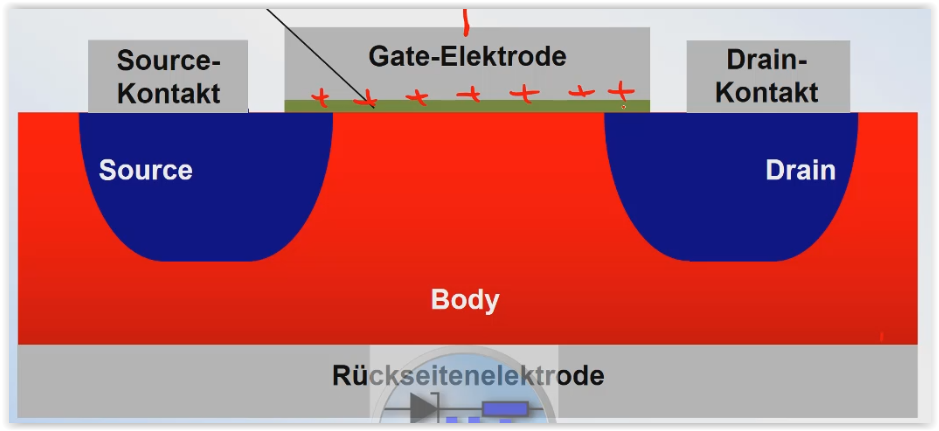
\includegraphics[width=1.05\linewidth]{misfet_feldeffekt_a.png}
		      \caption{MISFET Feldeffekt \protect\cite{MIKRO2}}
		      \label{fig:misfet_feldeffekt_a}
				\end{minipage}%
				\begin{minipage}{.5\textwidth}
				  \centering
				  \captionsetup{justification=centering}
				  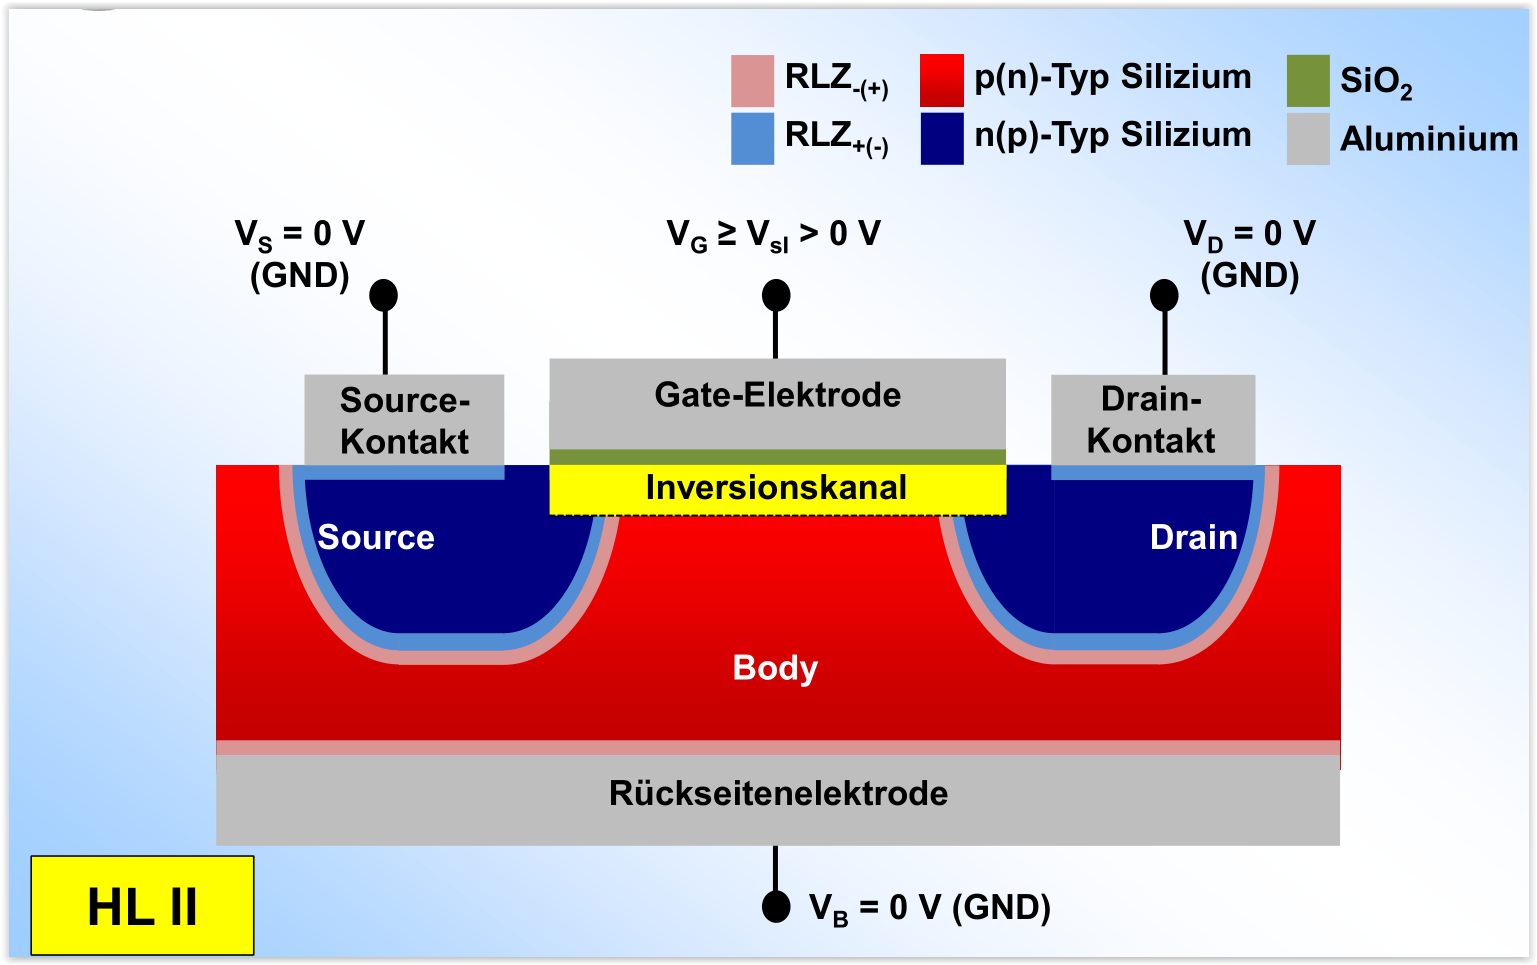
\includegraphics[width=0.77\linewidth]{misfet_inversionskanal.png}
				  \caption{MISFET Inversionskanal \protect\cite{MIKRO2}}
				  \label{fig:misfet_inversionskanal}
				\end{minipage}%
		  \end{figure}
		  
   \subsection{Some facts}
   \begin{itemize}
     \item Mit steigender Dotierung senkt sich die Diffusionslänge
     \item Diffusionslängen:
	     \begin{table}[H]
		     \centering
		     \begin{tabular}{c | l}
		       Hochdotiertes Si, Ge & $\approx 1-3\mu m$ \\
		       Schwachdotiertes Si, Ge & $\approx 100-300\mu m$ 
		     \end{tabular}
	     \end{table}
   \end{itemize}
\newpage	

  \section{17. Juli 2018: Vorlesung 12}
  \subsection{Fortsetzung zu \ref{subsubs:misfet_feldeffekt}}
  Im Folgenden Beispiel sei der Body mit $N_A = 1\cdot 10^{16}cm^{-3}$ dotiert. Wie bereits weiter oben erwähnt trennt das elektrische Feld die vom Halbleiter generierten Elektronen/Loch-Paare. Die Elektronen werden nach oben zur Grenzfläche gesaugt und die Löcher nach unten hin weg beschleunigt. Dort diffundieren sie aufgrund des entstehenden Konzentrationsgradienten zur Rückseitenelektrode und fließen über die Erde ab. So wird der Kanal Stück für Stück negativ aufgeladen. Wie stark negativ aufgeladen wird hängt von der Gate-Spannung ab. Es gibt 5 konkrete Zustände die so eine MOS-Kapazität dabei annehmen kann.
  \begin{itemize}
    \item[1) ] Schwache Verarmung: Zunächst verhält es sich wie ein leicht schwächer dotierter p-Typ Halbleiter. Löcher sind auch nahe der Grenzfläche immernoch mehr vorhanden als Elektronen, allerdings rekombinieren die durch die Influenz des el. Feldes angezogenen Elektronen mit den Löchern und die p-Dotierung wird geringer. P-Typ Leitfähigkeit ist aber immer noch dominierend.
    \item[2) ] Starke Verarmung: Der Bereich verhält sich immernoch p-Typ dotiert, allerdings jetzt nur noch sehr schwach.
    \item[3) ] Intrinsischer Fall: Sobald exakt $10^{16}cm^{-3}$ Elektronen zur Grenzfläche gezogen wurden verhält sich der Halbleiter intrinsisch. Allgemein, sobald gleich viel Löcher wie Elektronen dotiert wurden.
    \item[4) ] Schwache Inversion: Sobald etwas mehr als $10^{16}cm^{-3}$ Elektronen zur Grenzfläche gezogen wurden verhält sich das Material in dem Bereich wie ein schwach dotierter n-Typ Halbleiter. Allgemein ausgedrückt, sobald mehr Elektronen als Löcher in dem Kanalbereich sind.
    \item[5) ] Starke Inversion: Verhält sich wie ein stark dotierter N-Typ Halbleiter. Beim MOSFET ist der Bereich so definiert, dass die Leitfähigkeit sich komplett umdreht. Also hier im Beispiel von $N_A = 10^{16}cm^{-3}$ zu $N_D = 10^{16}cm^{-3}$. Das heißt in unserem Beispiel müssten $2\cdot 10^{16}cm^{-3}$ Elektronen in den Kanal gezogen werden. Die Spannung die nötig ist um diesen Zustand einzustellen nennt man Schwellwertspannung.
  \end{itemize}
  Wird eine negative Spannung an die Gate-Elektrode angelegt werden durch das el. Feld die Löcher an die Grenzfläche gezogen während Elektronen über die Erde wegdiffundiert werden. Der Kanal wird dann p-dotiert aufgeladen. Man spricht hier von Akkumulation (im Gegensatz zu Inversion). Die grenzflächennahe Schicht verhält sich wie ein noch stärker p-Typ dotierter Halbleiter.
  
  \begin{figure}[H] 
			\centering
			\begin{minipage}{.5\textwidth}
			  \centering
			  \captionsetup{justification=centering}
	      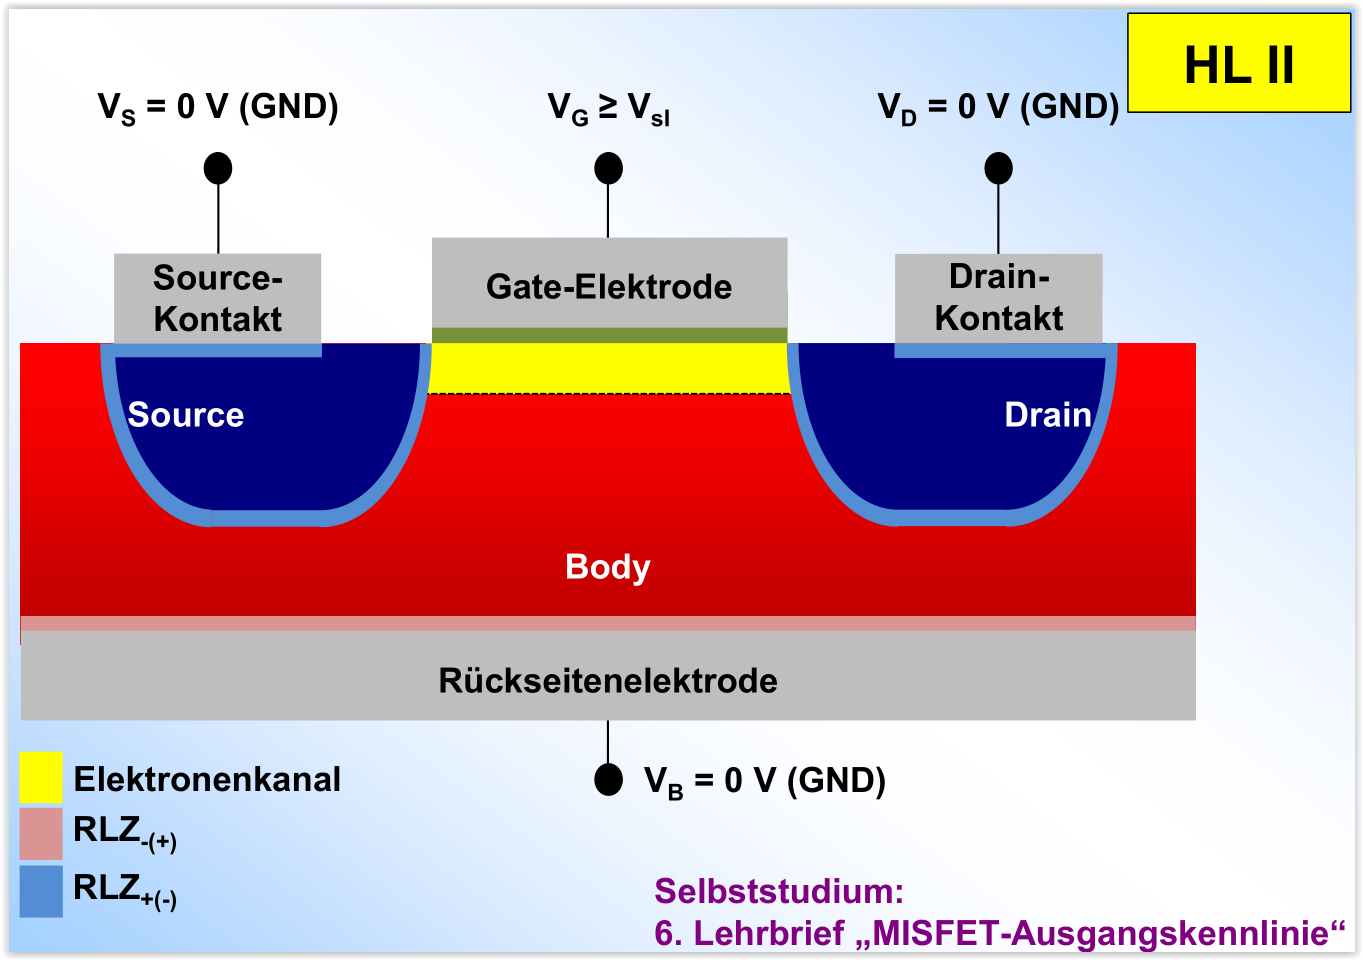
\includegraphics[width=0.9\linewidth]{misfet_inversion_full.png}
	      \caption{MISFET Inversionskanal \protect\cite{MIKRO2}}
	      \label{fig:misfet_inversion_full}
			\end{minipage}%
			\begin{minipage}{.5\textwidth}
			  \centering
			  \captionsetup{justification=centering}
			  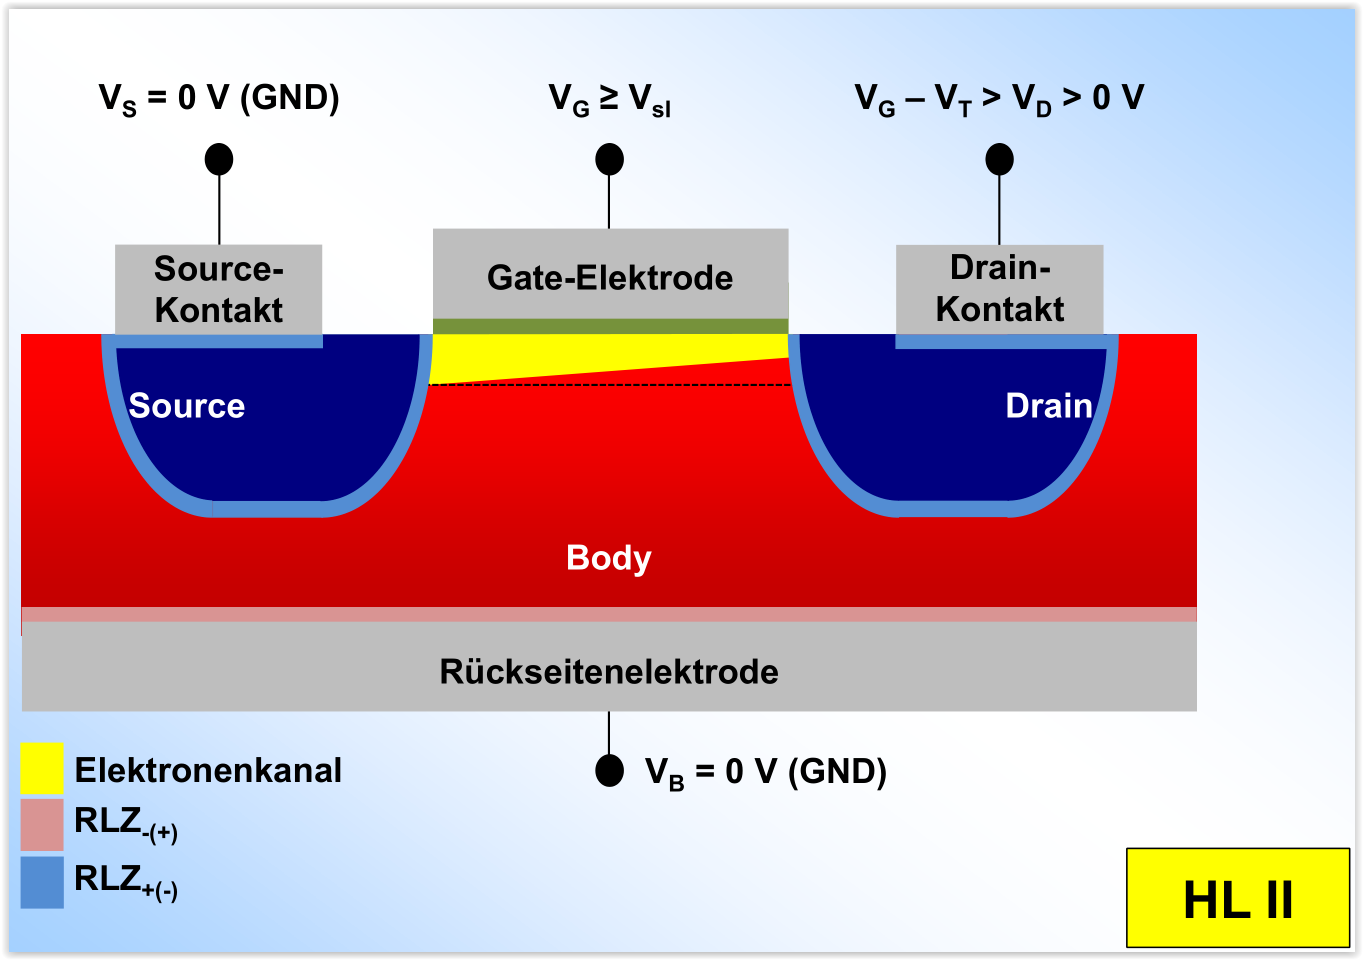
\includegraphics[width=0.9\linewidth]{misfet_inversion_less.png}
			  \caption{MISFET Inversionskanal  \protect\cite{MIKRO2}}
			  \label{fig:misfet_inversion_less}
			\end{minipage}%
	  \end{figure}
	  Legt man nun an Drain ein Spannung größer Null an fließen Elektronen von Source nach Drain und zwar hauptsächlich durch den Inversionskanal, da dort der Widerstand sehr viel geringer ist. Über den Body fließen so gut wie keine Elektronen, da einer der beiden PN-Übergänge immer in Sperrrichtung ist. Damit entspricht der Mosfet einer Verschaltung von Widerständen und die Kennlinie wäre damit ein linearer Zusammenhang. Tatsächlich hat ein MOSFET nur im Anfangsbereich mit kleinen Drain-Source Spannungen einen linearen Zusammenhhang. Bei steigender Drain-Source Spannung flachen die Kurven aber ab und knicken ein (siehe Abbildung \ref{fig:misfet_kennlinie}).
	  \begin{figure}[H]
		  \centering
		  \captionsetup{justification=centering}
		  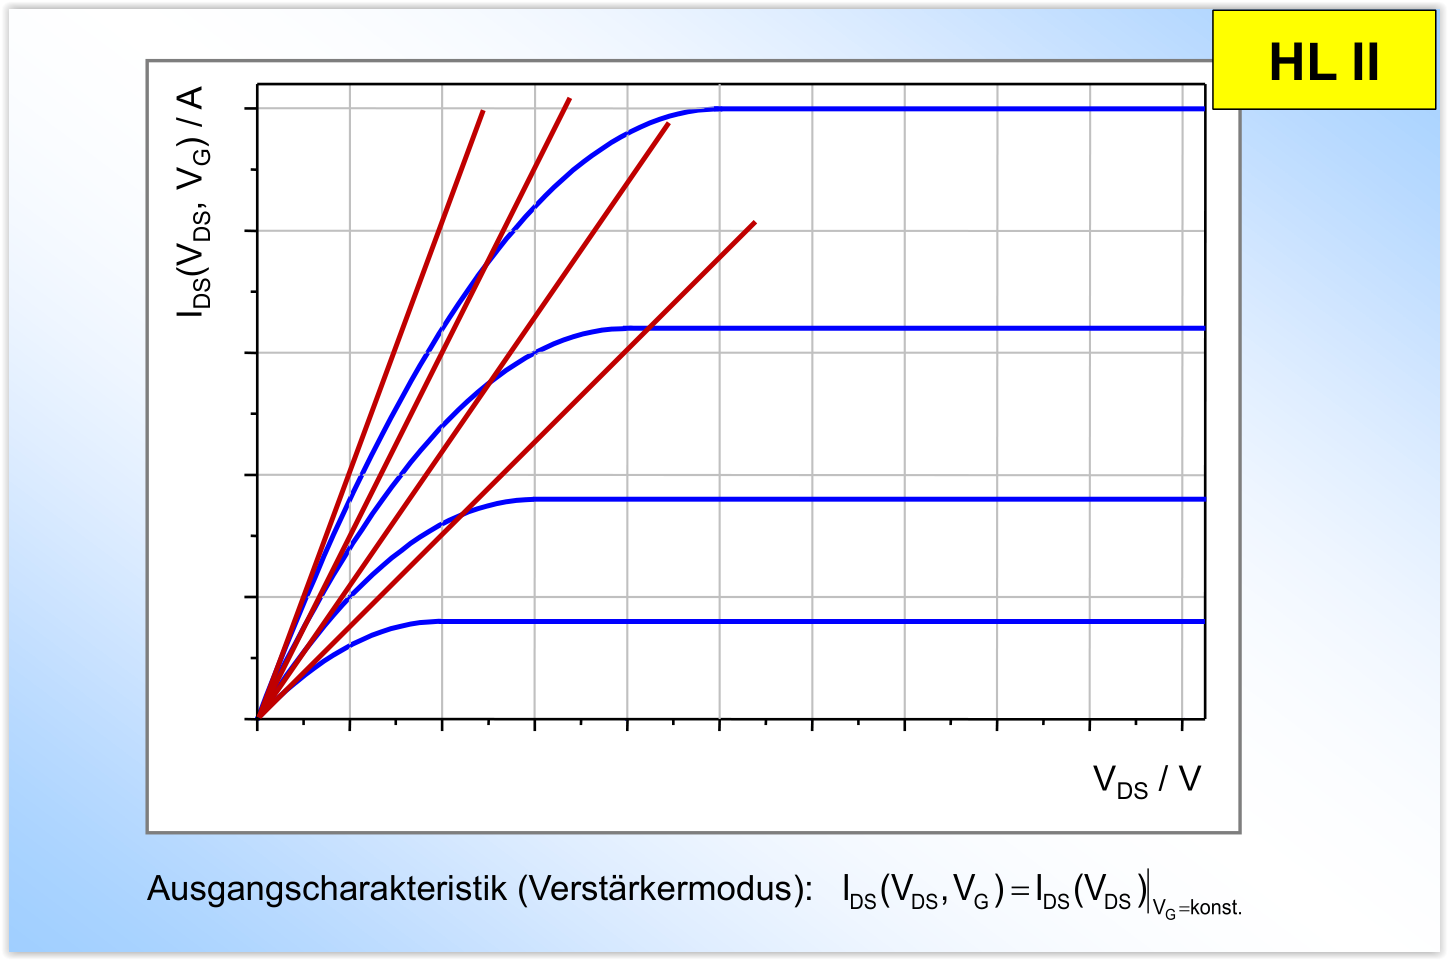
\includegraphics[width=0.8\linewidth]{misfet_kennlinie.png}
		  \caption{MISFET Stromkennlinie \protect\cite{MIKRO2}}
		  \label{fig:misfet_kennlinie}
		\end{figure}
		Man erkennt in Abbildung \ref{fig:misfet_kennlinie} weiterhin, dass es für jede Kurve einen Punkt gibt, ab dem der Strom nicht mehr weiter steigt. Zusammengefasst heißt das, wenn die Drain-Source Spannung klein genug ist, verhält der MOSFET sich ohmsch. In einem Übergangsbereich steigt der Strom weiterhin, allerdings nicht mehr in einem linearen Zusammenhang. Ab einem Punkt verhält sich der Transistor dann nicht ohmsch. In dem Zwischenbereich geht die Kennlinie also von einem ohmschen in ein nicht ohmsches Verhalten sukzessive über.\newline 
		Damit ein ohmsches Verhalten sichtbar ist, muss die Ladungsträgerkonzentrationsverteilung homogen sein und beim Anlegen eines elektrischen Feldes müssen sich die Elektronen alle mit einer mittleren Driftgeschwindigkeit bewegen. Dies ist offensichtlich für kleine $V_{DS}$ der Fall, für größer werdende $V_{DS}$ allerdings nicht mehr. Entweder muss die Beweglichkeit also abnehmen oder die Ladungsträgerkonzentration verändert sich (aufgrund des geringeren Stromflusses als erwartet also abnehmen). Erhöht man nun die Drain Spannung langsam bis sie auf dem selben Niveau wie die Gate Spannung ist, sinkt die Spannung ganz rechts am Kanal immer weiter bis sie $0V$ ist, während ganz links im Kanal die volle Gate-Spannung abfällt. Da die Ladung mit
		\begin{equation}
		  Q = C_{gox}\cdot U
		\end{equation}
		gegeben ist, erhält man einen Ladungsverlauf wie er in Abbildung \ref{fig:misfet_inversion_less} bzw. für den Fall dass ganz rechts tatsächlich $0V$ anliegen und somit keine Ladung mehr vorhanden ist in Abbildung \ref{fig:misfet_inversion_half} angedeutet ist. Abbildung \ref{fig:misfet_inversion_symbol} soll diesen Ladungsverlauf illustrieren.
	  \begin{figure}[H] 
			\centering
			\begin{minipage}{.5\textwidth}
			  \centering
			  \captionsetup{justification=centering}
	      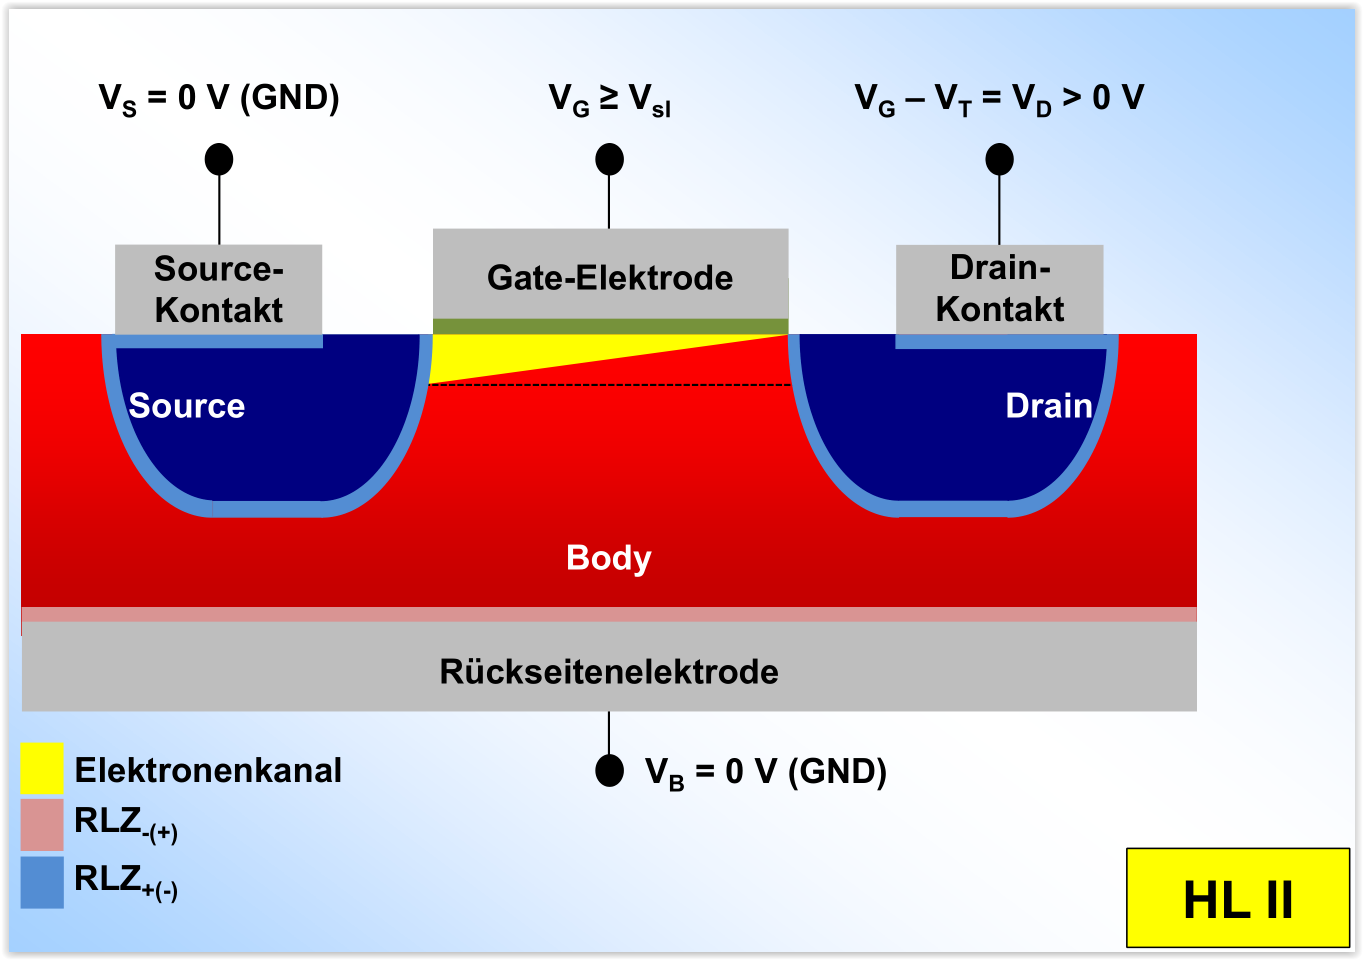
\includegraphics[width=0.88\linewidth]{misfet_inversion_half.png}
	      \caption{MISFET Feldeffekt \protect\cite{MIKRO2}}
	      \label{fig:misfet_inversion_half}
			\end{minipage}%
			\begin{minipage}{.5\textwidth}
			  \centering
			  \captionsetup{justification=centering}
			  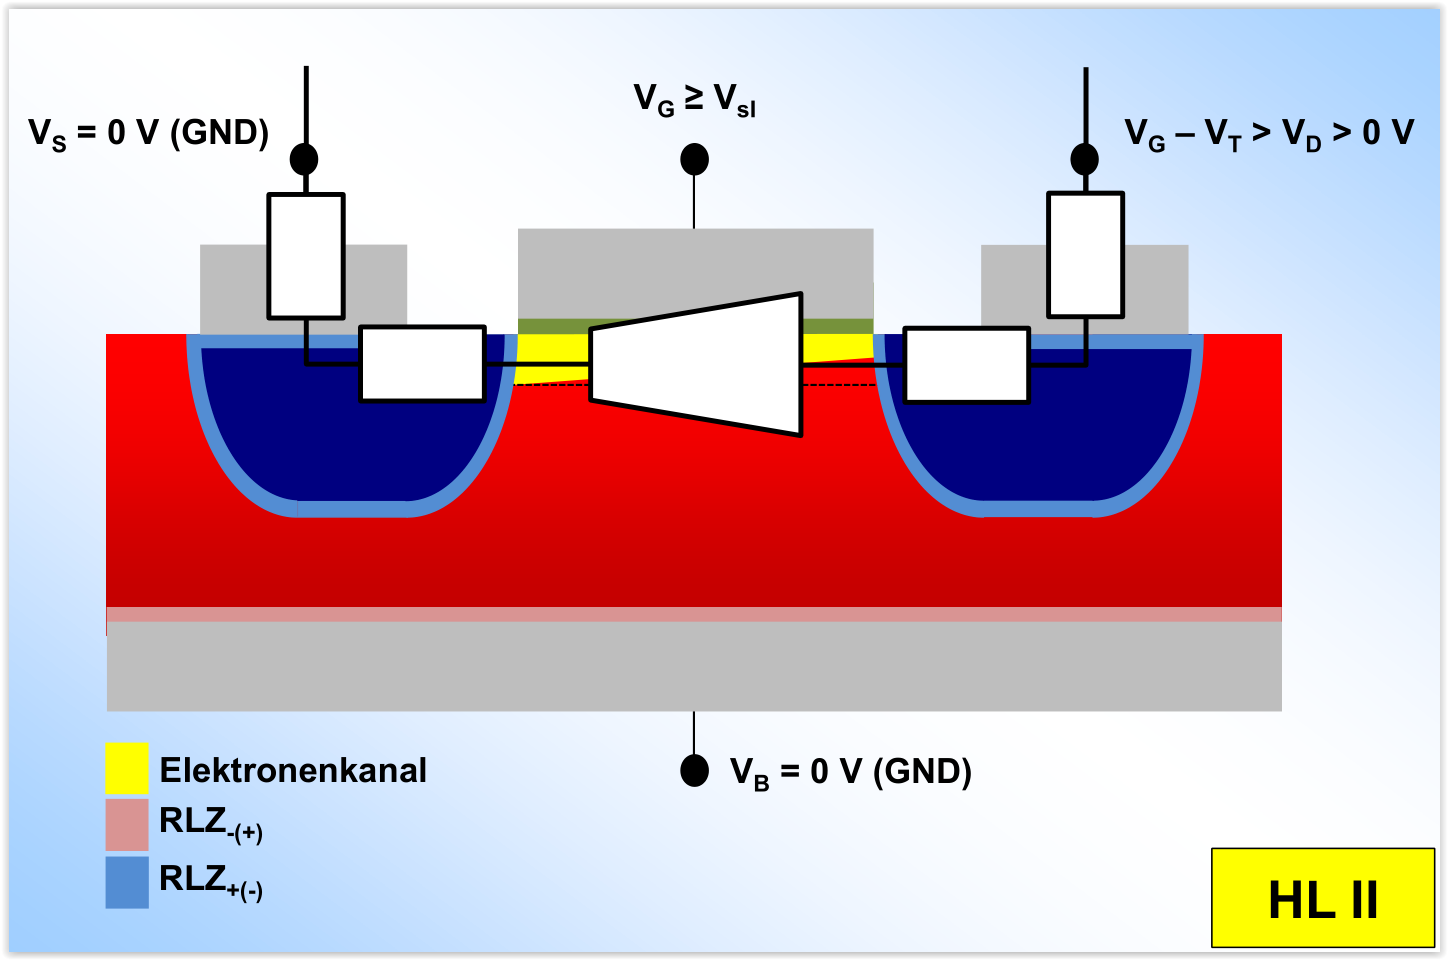
\includegraphics[width=0.92\linewidth]{misfet_inversion_symbols.png}
			  \caption{MISFET Symbole \protect\cite{MIKRO2}}
			  \label{fig:misfet_inversion_symbol}
			\end{minipage}%
	  \end{figure}
	  Warum fließt nun immernoch Strom? Während die ohmsche Transportkomponente immer geringer wurde, wurde die Diffusion immer stärker, denn durch den Ladungsverlauf bildet sich ein starker Konzentrationsgradient. Der ohmsche Transport kommt dann zwar komplett zum erliegen aber durch einen konstanten Konzentrationsgradient bleibt dann auch der Strom konstant. 
\newpage

\chapter{Anhänge}
\section{Hilfstabellen}
	\subsection{Abkürzungen/Formelzeichen} \label{ch:names}
	\renewcommand{\arraystretch}{1.5}
	\begin{longtable} {|p{2cm}|p{3cm}|p{8.4cm}|} \hline
	% Definition des Tabellenkopfes auf der ersten Seite
	%Spaltenbezeichnungen
	\textbf{Zeichen} & \textbf{Einheit} & \textbf{Bedeutung} \\
	\hline
	\endfirsthead % Erster Kopf zu Ende
	% Definition des Tabellenkopfes auf den folgenden Seiten
	\caption{Abkürzungen/Formelzeichen}\\ \hline
	%Spaltenbezeichnungen
	\textbf{Zeichen} & \textbf{Einheit} & \textbf{Bedeutung} \\
	\hline
	\endhead % Zweiter Kopf ist zu Ende
	\multicolumn{3}{r}{Fortsetzung auf Folgeseite}\\
	\endfoot
	\hline
	%\multicolumn{3}{r}{Ende} \\
	\endlastfoot
	
	%a-g
	$A$ & $m^2$ & Fläche \\ \hline
	$a$ & $\frac{m}{s^2}$ & Beschleunigung \\ \hline
	$b$ & $\frac{cm^2}{Vs}$ & Ladungsträgerbeweglichkeit \\ \hline
	$d$ & $m$ & Dicke \\ \hline
	$D_n$ & $\frac{m^2}{s}$ & Diffusionskonstante für Elektronen \\ \hline
	$D_p$ & $\frac{m^2}{s}$ & Diffusionskonstante für Löcher \\ \hline
	$e$ & $C$ & Elementarladung \\ \hline
	$E$ & $\frac{N}{C} = \frac{VAs}{mAs} = \frac{V}{m}$ & Elektrische Feldstärke \\ \hline
	$E_c$ & $eV$ & Leitungsbandkante \\ \hline
	$E_F$ & $eV$ & Fermi-Energie \\ \hline
	$E_g$ & $eV$ & Energie der Bandlücke \\ \hline
	$E_v$ & $eV$ & Valenzbandkante \\ \hline
	$f$ & $Hz$ & Frequenz \\ \hline
	$\vec{F}$ & $N = \frac{kgm}{s^2}$ & Kraft \\ \hline
	$G$ & $\frac{A}{V} = \frac{1}{\Omega} = S$ & Leitwert \\ \hline
	
	%h-n
	$h$ & $eVs$ & Planksches Wirkungsquantum\\ \hline
	$\hbar$ & $eVs$ & Dirac-Konstante \\ \hline
	$i$ & $A$ & Elektrischer Strom \\ \hline
	$j$ & $\frac{A}{m2}$ & Elektrische Stromdichte \\ \hline
	$J_n$ & $\frac{A}{m2}$ & Elektronenstromdichte \\ \hline
	$J_p$ & $\frac{A}{m2}$ & Löcherstromdichte \\ \hline
	$J_{diff}$ & $\frac{A}{m2}$ & Diffusionsstromdichte \\ \hline
	$J_{part}$ & $\frac{A}{m2}$ & Partikelstromdichte \\ \hline
	$J_to$ & $\frac{A}{m2}$ & Totale Stromdichte \\ \hline
	$J_r$ & $\frac{A}{m2}$ & Rekombinationsstromdichte \\ \hline
	$J_{drift}$ & $\frac{A}{m2}$ & Driftstromdichte \\ \hline
	$l$ & $m$ & Länge \\ \hline
	$L$ & $m$ & Minoritätsladungsträgerdiffusionslänge \\ \hline
	$L_n$ & $m$ & Diffusionslänge Elektronen \\ \hline
	$L_p$ & $m$ & Diffusionslänge Löcher \\ \hline
	
	%m-u
	$n$ & ... & Elektronenkonzentration \\ \hline
	$n_i$ & ... & Intrinsische Ladungsträgerdichte \\ \hline
	$n_{id}$ & ... & Idealität einer Diode \\ \hline
  $N_A$ & $m^{-3}$ & Akzeptorendichte \\ \hline
  $N_D$ & $m^{-3}$ & Donatorendichte \\ \hline
	$N_C$ & $cm^{-3}$ & Effektive Zustandsdichte der Elektronen \\ \hline
	$N_V$ & $cm^{-3}$ & Effektive Zustandsdichte der Löcher \\ \hline
	$p$ & ... & Lochkonzentration \\ \hline
	$q$ & $C$ & Probeladung (in der Regel = $e$) \\ \hline
	$\vec{r}$ & $m$ & Weg \\ \hline
	$r$ & $\Omega$ & Differentieller Widerstand \\ \hline
	$R$ & $\Omega$ & Widerstand \\ \hline
	$R_F$ & $\frac{\Omega}{square}$ & Flächenwiderstand \\ \hline 
	$U$ & $V$ & Elektrische Spannung \\ \hline
	$U_g$ & $V$ & Gesamtspannung \\ \hline
	 
	%v-z
	$v$ & $\frac{m}{s}$ & Geschwindigkeit \\ \hline
	$v_D, v_d$ & $\frac{m}{s}$ & Driftgeschwindigkeit \\ \hline
	$w$ & $m$ & Weite bzw. Breite  \\ \hline
	$W$ & $Ws = J = \frac{kgm^2}{s^2}$ & Arbeit bzw. Energie \\ \hline
	
	%griechisch
	$\alpha$ & $\frac{1}{^{\circ} C}$ & Temperturkoeffizient des Ohmwiderstandes \\ \hline
	$\nu$ & $Hz$ & Hier Frequenz der Welle \\ \hline
	$\rho$ & $\frac{V cm}{A} = \Omega  cm$ & Spezifischer Widerstand \\ \hline
	$\rho_e$ & ... & Ladungsdichte \\ \hline
	$\kappa$ & $\frac{1}{\Omega cm} = \frac{S}{cm}$ & Spezifische Leitfähigkeit \\ \hline
	$\varepsilon_0$ & $\frac{As}{Vm}$ & Dielektrizitätskonstante im Vakuum \\ \hline
	$\varphi$ & $V$ & Elektrisches Potential \\ \hline
	$\tau$ & $s$ & Stoßzeit \\ \hline
	$\tau$ & $s$ & Minoritätsladungsträgerlebensdauer \\ \hline
	$\mu$ & $\frac{cm^2}{Vs}$ & Beweglichkeit \\ \hline
	%Sonderzeichen
	\end{longtable}
	\renewcommand{\arraystretch}{1}
	
	\subsection{Wichtige Donatoren und Akzeptoren} \label{ch:don/acc}
	\renewcommand{\arraystretch}{1.5}
	\begin{longtable} {|p{2cm}|p{3cm}|p{8.4cm}|} \hline
	% Definition des Tabellenkopfes auf der ersten Seite
	%Spaltenbezeichnungen
	\textbf{Ch. Sym.} & \textbf{Name} & \textbf{Typ} \\
	\hline
	\endfirsthead % Erster Kopf zu Ende
	% Definition des Tabellenkopfes auf den folgenden Seiten
	\caption{Wichtige Donatoren und Akzeptoren}\\ \hline
	%Spaltenbezeichnungen
	\textbf{Zeichen} & \textbf{Einheit} & \textbf{Bedeutung} \\
	\hline
	\endhead % Zweiter Kopf ist zu Ende
	\multicolumn{3}{r}{Fortsetzung auf Folgeseite}\\
	\endfoot
	\hline
	%\multicolumn{3}{r}{Ende} \\
	\endlastfoot
	$B$ & Bor & Akzeptor \\ \hline
	$Al$ & Alluminium & Akzeptor \\ \hline
	$Ga$ & Gallium & Akzeptor \\ \hline
	$In$ & Indium & Akzeptor \\ \hline
	$P$ & Phosphor & Donator \\ \hline
	$As$ & Arsen & Donator \\ \hline
	$Sb$ & Antimon & Donator \\ \hline
	$Bi$ & Wismut & Donator \\ \hline
	\end{longtable}
	\renewcommand{\arraystretch}{1}
	\newpage
	\subsection{Effektive Massen} \label{ch:don/acc}
	\renewcommand{\arraystretch}{1.5}
	\begin{longtable} {|p{2cm}|p{3cm}|p{8.4cm}|} \hline
	% Definition des Tabellenkopfes auf der ersten Seite
	%Spaltenbezeichnungen
	\textbf{Band} & \textbf{Wert} & \textbf{Element} \\
	\hline
	\endfirsthead % Erster Kopf zu Ende
	% Definition des Tabellenkopfes auf den folgenden Seiten
	\caption{Effektive Massen}\\ \hline
	%Spaltenbezeichnungen
	\textbf{Band} & \textbf{Wert} & \textbf{Element} \\
	\hline
	\endhead % Zweiter Kopf ist zu Ende
	\multicolumn{3}{r}{Fortsetzung auf Folgeseite}\\
	\endfoot
	\hline
	%\multicolumn{3}{r}{Ende} \\
	\endlastfoot
	$\frac{m_n^*}{m_0}$ & $1,08$ & Silizium \\ \hline
	$\frac{m_n^*}{m_0}$ & $1,561$ & Germanium \\ \hline
	$\frac{m_n^*}{m_0}$ & $1,067$ & Gallium-Arsenid \\ \hline
	$\frac{m_p^*}{m_0}$ & $1,10$ & Silizium \\ \hline
	$\frac{m_p^*}{m_0}$ & $1,291$ & Germanium \\ \hline
	$\frac{m_p^*}{m_0}$ & $1,473$ & Gallium \\ \hline
	\end{longtable}
	\renewcommand{\arraystretch}{1}
	
	\subsection{Bandlücken wichtiger Materialien} \label{ch:gaps}
	\renewcommand{\arraystretch}{1.5}
	\begin{longtable} {|p{2cm}|p{3cm}|p{8.4cm}|} \hline
	% Definition des Tabellenkopfes auf der ersten Seite
	%Spaltenbezeichnungen
	\textbf{Zeichen} & \textbf{Wert in \text{e}V} & \textbf{Material} \\
	\hline
	\endfirsthead % Erster Kopf zu Ende
	% Definition des Tabellenkopfes auf den folgenden Seiten
	\caption{Bandlücken wichtiger Materialien}\\ \hline
	%Spaltenbezeichnungen
	\textbf{Zeichen} & \textbf{Einheit} & \textbf{Bedeutung} \\
	\hline
	\endhead % Zweiter Kopf ist zu Ende
	\multicolumn{3}{r}{Fortsetzung auf Folgeseite}\\
	\endfoot
	\hline
	%\multicolumn{3}{r}{Ende} \\
	\endlastfoot
	$E_{g,SiO_2}$ & $9$ & Siliziumdioxid \\ \hline
	$E_{g,C}$ & $5,47$ & Diamant \\ \hline
	$E_{g,CdS}$ & $2,42$ & Cadmiumsulfid \\ \hline
	$E_{g,GaP}$ & $2,26$ & Galliumphosphid \\ \hline
	$E_{g,GaAs}$ & $1,42$ & Gallium-Arsenid \\ \hline
	$E_{g,InP}$ & $1,35$ & Indiumphosphid \\ \hline
	$E_{g,Si}$ & $1,12$ & Silizium \\ \hline
	$E_{g,Ge}$ & $0,66$ & Germanium \\ \hline
	$E_{g,InSb}$ & $0,17$ & Indiumantimonid \\ \hline
	\end{longtable}
	\renewcommand{\arraystretch}{1}
	
	\subsection{Eckdaten wichtiger Halbleiter} \label{ch:eckd}
	\renewcommand{\arraystretch}{1.5}
	\begin{longtable} {|p{2cm}|p{2.6cm}|p{2.6cm}|p{2.6cm}|p{2.7cm}|} \hline
	% Definition des Tabellenkopfes auf der ersten Seite
	%Spaltenbezeichnungen
	\textbf{Ch. Sym.} & \textbf{$E_g$ in $\bracks{eV}$} & \textbf{$N_C$ in $\bracks{cm^{-3}}$} & \textbf{$N_V$ in $\bracks{cm^{-3}}$} & \textbf{$n_i$ in $\bracks{cm^{-3}}$} \\
	\hline
	\endfirsthead % Erster Kopf zu Ende
	% Definition des Tabellenkopfes auf den folgenden Seiten
	\caption{Eckdaten wichtiger Halbleiter}\\ \hline
	%Spaltenbezeichnungen
	\textbf{Ch. Sym.} & \textbf{$E_g$ in $\bracks{eV}$} & \textbf{$E_g$ in $\bracks{eV}$} & \textbf{$E_g$ in $\bracks{eV}$} & \textbf{$E_g$ in $\bracks{eV}$} \\
	\hline
	\endhead % Zweiter Kopf ist zu Ende
	\multicolumn{3}{r}{Fortsetzung auf Folgeseite}\\
	\endfoot
	\hline
	%\multicolumn{3}{r}{Ende} \\
	\endlastfoot
	Si & $1,124$ & $2,81 \cdot 10^{19}$ & $2,88 \cdot 10^{19}$ & $1,04 \cdot 10^{10}$ \\ \hline
	Ge & $0,67$ & $1,05 \cdot 10^{19}$ & $3,92 \cdot 10^{18}$ & $1,55 \cdot 10^{13}$ \\ \hline
	GaAs & $1,424$ & $4,33 \cdot 10^{17}$ & $8,13 \cdot 10^{18}$ & $2,04 \cdot 10^{6}$ \\ \hline
	\end{longtable}
	\renewcommand{\arraystretch}{1}
	\newpage
\subsection{Niederfeld- und Niederdotierungsbeweglichkeiten ($T = 300K$)} \label{ch:bewegl.}
	\renewcommand{\arraystretch}{1.5}
	\begin{longtable} {|p{2.4cm}|p{3.5cm}|p{3.5cm}|p{3.5cm}|} \hline
	% Definition des Tabellenkopfes auf der ersten Seite
	%Spaltenbezeichnungen
	\textbf{$n/p$} & \textbf{Si} & \textbf{Ge} & \textbf{GaAs} \\
	\hline
	\endfirsthead % Erster Kopf zu Ende
	% Definition des Tabellenkopfes auf den folgenden Seiten
	\caption{Niederfeld- und Niederdotierungsbeweglichkeiten}\\ \hline
	%Spaltenbezeichnungen
	\textbf{$n/p$} & \textbf{Si} & \textbf{Ge} & \textbf{GaAs} \\
	\hline
	\endhead % Zweiter Kopf ist zu Ende
	\multicolumn{3}{r}{Fortsetzung auf Folgeseite}\\
	\endfoot
	\hline
	%\multicolumn{3}{r}{Ende} \\
	\endlastfoot
	  $\mu_n \bracks{\frac{cm^2}{Vs}}$ & $1340$ & $3900$ & $8000$ \\ \hline	
	  $\mu_p \bracks{\frac{cm^2}{Vs}}$ & $460$ & $1900$ & $400$ \\ \hline	
	\end{longtable}
	\renewcommand{\arraystretch}{1}	
	
	\subsection{Konstanten} \label{ch:constants}
	\renewcommand{\arraystretch}{1.5}
	
	\begin{longtable} {|p{0.6cm}|p{4.4cm}|p{8.4cm}|} \hline
	% Definition des Tabellenkopfes auf der ersten Seite
	%Spaltenbezeichnungen
	\textbf{Ze.} & \textbf{Wert} & \textbf{Bedeutung}\\
	\hline
	\endfirsthead % Erster Kopf zu Ende
	% Definition des Tabellenkopfes auf den folgenden Seiten
	\caption{Konstanten}\\ \hline
	%Spaltenbezeichnungen
	\textbf{Ze.} & \textbf{Wert} & \textbf{bedeutung}\\
	\hline
	\endhead % Zweiter Kopf ist zu Ende
	\multicolumn{3}{r}{Fortsetzung auf Folgeseite}\\
	\endfoot
	\hline
	%\multicolumn{3}{r}{Ende} \\
	\endlastfoot
	
	%a-g
	$c$ & $2,998...\cdot 10^8 \bracks{frac{m}{s}}$ & Lichtgeschwindigkeit\\ \hline
	$e,q$ & $1,602176...\cdot 10^{-19}\bracks{C}$ & Elementarladung\\ \hline
	$e,q$ & $1,602176...\cdot 10^{-19}\bracks{J}$ & Elementarladung\\ \hline
	%h-n
	$h$ & $6,63 \cdot 10^{-34} \bracks{Js}$ & Planck-Konstante\\ \hline
	$h$ & $4,136...\cdot 10^{-15} \bracks{eVs}$ & Planck-Konstante\\ \hline
	$\hbar$ & $\frac{h}{2\pi}$ & Plancksches Wirkungsquantum\\ \hline
	$k$ & $8,6173 \cdot 10^{-5} \bracks{\frac{eV}{K}}$ & Boltzmann Konstante\\ \hline
	$kT$ & $25,85 \bracks{meV}$ & mit der Boltzmann Konstante und $T=300K$ \\ \hline
	%m-u
	$m_0$ & $9,11 \cdot 10^{-31} \bracks{kg}$ & Elektronenmasse\\ \hline
	 
	%v-z
	
	%griechisch
	$\varepsilon_0$ & $8,854..\cdot 10^{-12}\bracks{\frac{As}{Vm}}$ & Dielektrizitätskonstante des Vakuuums \\ \hline
	$\varepsilon_{Si}$ & $11,90$ & Korrekturfaktor Dielektrizitätskonstante für Silizium\\ \hline
	%Sonderzeichen
	\end{longtable}
	\renewcommand{\arraystretch}{1}
\section{Graphiken}
  \begin{figure}[H]
		  \centering
		  \captionsetup{justification=centering}
		  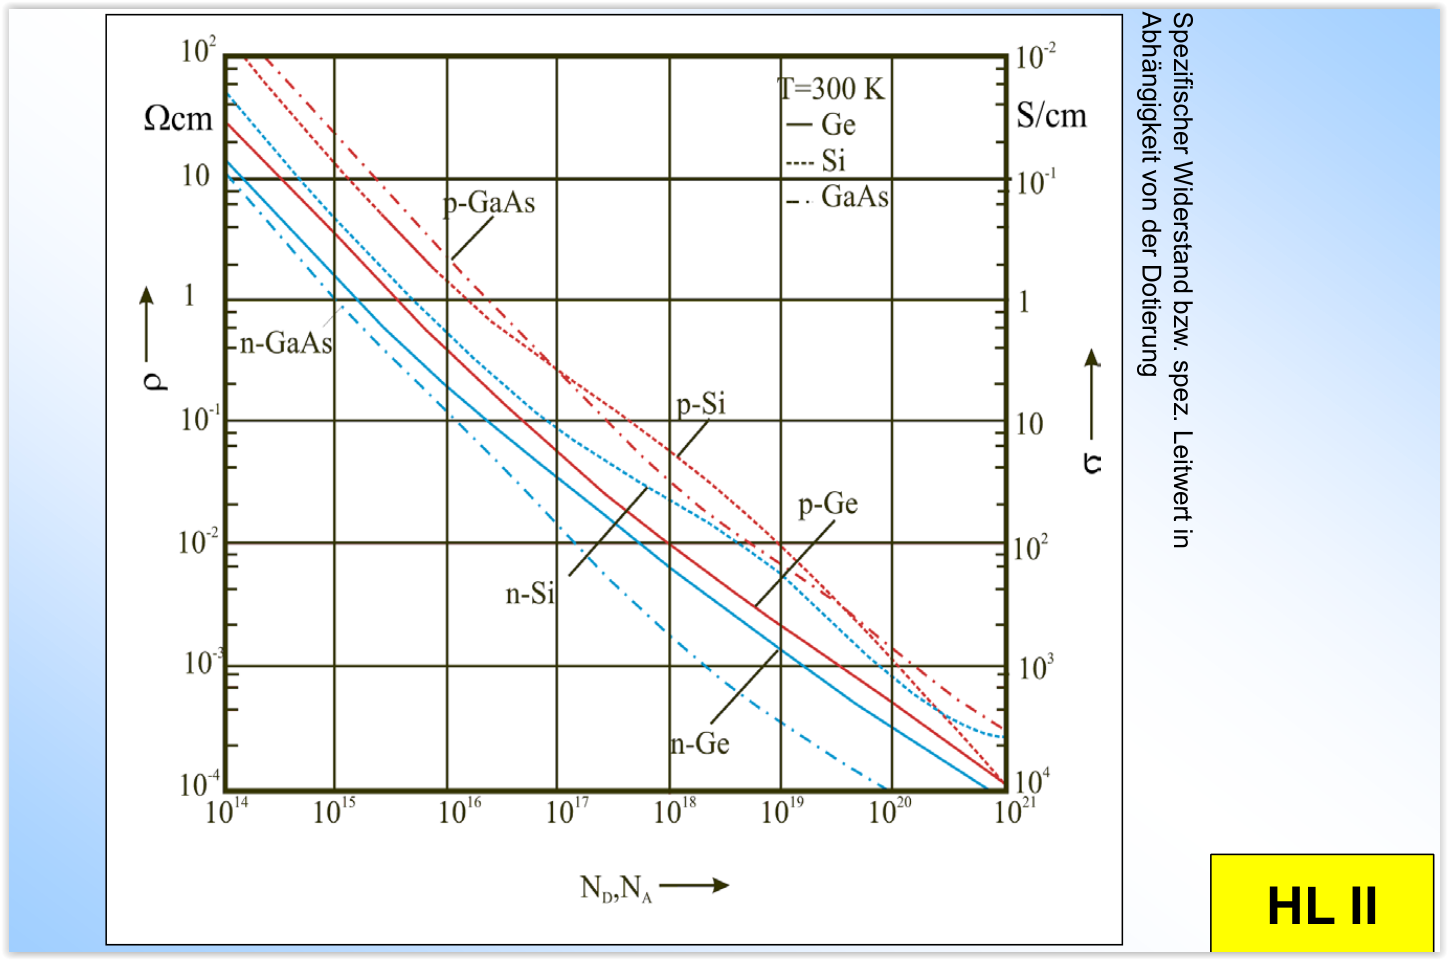
\includegraphics[width=1\linewidth]{dotierteHalbleiter_spezWid.png}
		  \caption{Spezifischer Widerstand dotierter Halbleiter}
		  \label{fig:dotierteHalbleiter_spezWid}
		\end{figure}


\bibliography{lit}

\end{document}
